% =====================================================================
%  FORMA - Specialized Project (CO4029) report
%  Ho Chi Minh City University of Technology (HCMUT) - VNU-HCM
%
%  Compile: pdflatex -> bibtex -> pdflatex -> pdflatex
%           (or: latexmk -pdf main.tex)
%
%  hcmut-thesis.cls is the faculty template's own file, byte for byte.
%  It is never modified. Everything this report needs is added here.
%
%  The chapter sources in chapters/ch*.tex are GENERATED from the
%  Markdown in docs/report/ by md2tex.py. Edit the Markdown, not the
%  .tex. The front matter and appendices in chapters/front and
%  chapters/back are written by hand and are not generated.
% =====================================================================
\documentclass[english,final]{hcmut-thesis}

\usepackage{amsmath,amssymb}
\usepackage{booktabs}
\usepackage{array}
\usepackage{longtable}
\usepackage{listings}
\usepackage[nameinlink]{cleveref}

\graphicspath{{graphics/}}

% Sections are numbered to subsection depth, because the prose refers to
% subsections by number. The contents list stops at section, because a
% contents page listing every subsection is a wall.
\setsecnumdepth{subsection}
\settocdepth{section}

% Generated tables are longtable, so they break across pages instead of
% floating away from the paragraph that introduces them.
\setlength{\LTcapwidth}{\textwidth}

\lstset{%
  basicstyle=\footnotesize\ttfamily,
  breaklines=true,
  breakatwhitespace=false,
  columns=fullflexible,
  keepspaces=true,
  showstringspaces=false,
  upquote=true,
  frame=leftline,
  framesep=8pt,
  xleftmargin=10pt,
  aboveskip=10pt,
  belowskip=10pt,
}

% The market sources in the bibliography are long hyphenated news URLs. The
% url package breaks only after a small set of characters by default, and a
% hyphen is not one of them, so each address is set as a single box that runs
% off the page. This adds the characters those addresses are actually made of.
% No \Urlmuskip here: stretchable glue between the characters lets a short
% line spread one address out across the full measure, which looks worse than
% the overflow it fixes.
\def\UrlBreaks{\do\/\do\-\do\.\do\_\do\?\do\&\do\=\do\+\do\:}

% Block quotations: indented and set smaller, not italicised, because
% several of them carry bold statements that italics would fight with.
\newenvironment{quoteblock}%
  {\begin{list}{}{\setlength{\leftmargin}{1.6em}%
                  \setlength{\rightmargin}{1.6em}%
                  \setlength{\listparindent}{0pt}%
                  \setlength{\parsep}{0.5\baselineskip}}%
   \item[]\small}%
  {\end{list}}

% ---------------------------------------------------------------------
%  Report information
% ---------------------------------------------------------------------
\reporttype{Specialized Project}
\title{FORMA: An AI-Powered Personal Training System\\on Mobile Devices}
\stumajor{Computer Science}
\reporttime{November 2026}

\supervisor{
  Assoc.~Prof.~Dr.~Quan Thanh Tho
}
\stuname{
  \begin{tabular}{@{}l@{\hspace{1em}}l@{}}
    Dinh Hoang Quan & -- 2352986 \\
  \end{tabular}
}

\begin{document}
\coverpage%

\frontmatter%
\begin{preface}{Declaration}
  I hereby declare that this specialized project is my own work, carried out under the supervision of Assoc.~Prof.~Dr.~Quan Thanh Tho at the Faculty of Computer Science and Engineering, Ho Chi Minh City University of Technology -- Vietnam National University Ho Chi Minh City.

  \noindent All external sources and references used in this project have been properly acknowledged and cited.

  \noindent If any instance of plagiarism is found, I take full responsibility. Ho Chi Minh City University of Technology -- VNU-HCM is not responsible for any copyright violation that may have occurred in this work.

  \vspace{2cm}

  \begin{flushright}
    \begin{tabular}{c}
      Ho Chi Minh City, November 2026 \\
      \textit{\textbf{Dinh Hoang Quan}} \\
    \end{tabular}
  \end{flushright}
\end{preface}

\begin{preface}{Acknowledgements}
  % DRAFT. This is yours to rewrite in your own words before submission.
  I would like to thank my supervisor, Assoc.~Prof.~Dr.~Quan Thanh Tho, for the
  direction that shaped this project. His insistence that the report argue for
  its choices rather than merely describe them changed how the work was done,
  not only how it was written.

  \noindent I also thank my family for their support throughout the semester.
\end{preface}

\begin{preface}{Abstract}
  Most people who train do so without anyone watching them, and the faults
  that matter are the ones they cannot see themselves committing. A correction
  is only useful while the repetition is still happening, which gives a system
  about three hundred milliseconds from a fault appearing to the trainee
  hearing about it. No surveyed product delivers spoken coaching inside that
  window, publishes how its accuracy was evaluated, or states how a new
  exercise is added.

  FORMA is a mobile system that observes a trainee through the phone's camera
  and speaks a corrective cue during the set. This first phase delivers the
  perception and assessment path for three exercises: the bodyweight squat,
  the push-up and the front plank. Pose estimation runs entirely on the
  handset, movement assessment is geometric constraints declared per exercise
  rather than a learned classifier, and feedback is a pre-authored spoken cue
  selected by a discrete fault code with no language model in the live path.
  An exercise is added by authoring one specification file, which a single
  generic evaluator executes.

  The pose engine was chosen by measuring eight configurations of two engines
  on the target handset. The chosen configuration sustains 29.57 frames per
  second with a 95th-percentile per-frame latency of 27 milliseconds, against
  requirements of 22 frames per second and 65 milliseconds. Across ten
  recorded sets totalling 9,893 frames the engine returned a pose on every
  frame. Repetition counting was exact on all seven counting sets. Six
  technique faults were evaluated against the recordings. Precision was 0.990
  on the five faults judged frame by frame, no individual fault fell below
  0.957 against a requirement of 0.90, and every scripted condition was
  detected.

  Five of the six faults carry a criterion cited to published work; no
  threshold carries a source, and the specification format records that gap in
  its own fields rather than concealing it. The evaluation rests on one
  subject in one session, and an independent labelling pass by a certified
  trainer is agreed and outstanding. Both are stated as the boundary of the
  claim rather than left to be inferred.

  \vspace{1em}
  \noindent\textbf{Keywords:} on-device pose estimation, movement
  assessment, exercise technique feedback, declarative rule specification,
  mobile computer vision.
\end{preface}

\begin{preface}{Workload}
  % This is a solo project. The template's multi-student table is reduced
  % to one row rather than removed, because the faculty template expects
  % this section to exist.
  \begin{table}[h]
    \centering
    \renewcommand{\arraystretch}{1.4}
    % The template ships 4.2/2.4/6.2/2.4cm, which overflows the text block
    % by 27pt. Tasks narrowed by 1cm so the table fits the page.
    \begin{tabular}{|p{4.2cm}|p{2.4cm}|p{5.2cm}|p{2.4cm}|}
      \hline
      \textbf{Student Name} & \textbf{Student ID} & \textbf{Tasks} & \textbf{Contribution} \\
      \hline
      Dinh Hoang Quan & 2352986 &
        - Problem definition and scope \newline
        - Market and technology survey \newline
        - Design decisions and architecture \newline
        - Movement assessment design \newline
        - Mobile client implementation \newline
        - UI/UX design and prototype \newline
        - Testing, measurement and evaluation \newline
        - Report
        & 100\% \\
      \hline
    \end{tabular}
  \end{table}
\end{preface}


\tableofcontents
\clearpage
\listoffigures
\clearpage
\listoftables

\mainmatter%
\counterwithin{equation}{chapter}
\counterwithin{table}{chapter}
\counterwithin{figure}{chapter}

\chapter{Introduction and Problem}
\label{chap:1}

\section{Motivation}
\label{sec:1.1}

Most people who train do so without anyone watching them. That is the ordinary case rather than the deprived one, and it is the case this project is built for.

In Vietnam, 72 percent of people who exercise pay for it in some form, and 90 percent of those surveyed watch sport or fitness video online, from a nationwide survey of 1,406 respondents aged 13 to 65 conducted in May 2021 (Q and Me consumer survey, 2021)\cite{qandme2021fitness}. People are already paying for training and already looking for guidance through a screen. What they are not getting is anyone who can see them while they move.

The supervised alternative is becoming harder to reach rather than easier. The number of gyms nationwide fell from 105 to 88 in under a year (Q and Me retail report 2025, via CafeF)\cite{qandme2025retail}. Elite Fitness closed every branch in Ho Chi Minh City and Kickfit went from twelve locations to two (CafeF, 3 April 2026)\cite{cafef2026gyms}. Over the same period membership prices rose by about 4 percent while customers reduced what they spent (Ken Research, via CafeF)\cite{kenresearch2025membership}.

The arithmetic of personal training explains why. A monthly training budget of 300,000 to 3,000,000 VND is typical (Coc Coc survey, via CafeF)\cite{coccoc2025budget}, while a single session with a personal trainer is advertised at 250,000 to 1,500,000 VND by the gym chains themselves. Those advertised prices are not a survey, and they are asking prices, not what people pay. The order of magnitude is still the point. For most of that budget range, one or two supervised sessions a month exhausts it entirely. Continuous supervision is not a choice the majority is declining. It is a choice the majority does not have.

A phone, by contrast, is already in the room. It has a camera good enough to see a whole body, a processor fast enough to interpret what it sees, and a speaker the user is already wearing headphones for. The question this project asks is what a phone can usefully say to someone in the middle of a set.

\section{Problem Statement}
\label{sec:1.2}

A person training without a coach cannot see themselves, and this is a physical fact rather than a figure of speech. It holds across all three movements this project covers, and it gets worse as it goes.

In a squat the eyes face forward while the failures that matter occur at the hip, the knee and the torso, none of which is in view. In a push-up the head is down, so the line of the body behind it is out of sight entirely. In a plank the fault is a slow drift of the hips across thirty seconds or more, and the person holding the position has no reference for where their hips were when they started.

In each case the correction has to arrive while the movement is still happening. A squat repetition lasts two to three seconds, and after that there is nothing left to correct.

Three consequences follow, and they compound.

Faults persist because they are invisible to the person committing them. Someone who stops short of depth or lets the torso pitch forward has no signal that anything is wrong. The movement feels normal, because it is the movement they have always performed.

The cost arrives late. Repeated technique faults accumulate into injury rather than causing it immediately, which removes exactly the feedback that would otherwise prompt a correction. By the time the knee hurts, the thousand repetitions that produced it are already done.

There is no record of how well the work was done. Logging that three sets of ten were completed says nothing about whether they were completed well, so there is no basis on which to adjust the programme.

A human coach solves all of this, and four separate things stand between most people and one.

\begin{itemize}
\item Price. As 1.1 set out, one or two sessions a month spends a typical monthly training budget in full.
\item Schedule. A coach is available when the coach is available, so training happens where two calendars overlap rather than when the user decides to train.
\item Place. The coach is at the gym. Training at home, in a hotel room, or in the twenty minutes before work is training without them.
\item Fit. A coach is a person. Some talk through the whole set, some never explain why, and some are better with experienced lifters than with beginners. Changing coach means paying to begin again, and a beginner who is reluctant to be watched closely while they are still bad at the movement may not start at all.
\end{itemize}

None of these is a complaint about coaching. They are the reasons a motivated person ends up training alone despite wanting help.

The remedies available to someone training alone are each incomplete in their own way. A mirror gives one angle, and only while the user is looking into it, which is not the moment the fault occurs. Recording a set and watching it afterwards genuinely works, but it is post hoc: the repetitions it describes are finished and cannot be changed.

What is missing is something already where the user is at the moment they decide to train. It watches the movement, not the clock. It costs no more to use a second time. And it stays quiet when there is nothing worth saying. That is the problem this project addresses.

\section{Objectives}
\label{sec:1.3}

Six objectives for this phase, each stated so that its completion can be checked rather than asserted.

\textbf{O1. On-device perception.} A pose estimation pipeline running entirely on the mobile device, reaching a frame rate and a per-frame latency sufficient for feedback delivered while the user is still moving. Running on the device, not on a server, is itself part of the objective. It bounds latency, it removes a per-user running cost, and it keeps the user's video on the user's phone.

\textbf{O2. Movement assessment.} A layer that counts repetitions and detects technique faults for push-up, plank and bodyweight squat, designed so that adding a new exercise does not require hand-written rules.

\textbf{O3. Immediate spoken feedback.} A corrective cue delivered as speech, drawn from a bank of pre-authored lines, with no dependency on a large language model in the path between observing a fault and saying something about it.

\textbf{O4. The application, a server service and a user profile.} A mobile application carrying the session flow and the interface, a server-side service, and a user profile that stores session history.

\textbf{O5. Traceable fault definitions and a labelling protocol.} The technique fault set comes from a taxonomy that expert trainers already annotated in published work. None of it was invented here. With it comes a labelling protocol: the data used for evaluation is confirmed independently by a certified trainer.

\textbf{O6. A labelled dataset and a testing procedure.} A labelled video dataset, and a written procedure for measuring fault detection accuracy, end-to-end latency and session stability on real devices.

\section{Scope}
\label{sec:1.4}

\subsection{In scope for this phase}
\label{sec:1.4.1}

Three exercises: the bodyweight squat, the push-up and the front plank. All three are performed at floor level, need no equipment, can be recorded in any room, and are readable from a single viewpoint.

A single camera in a single position. The user places the phone to one side and the system reads the movement from that view. No second camera, no depth sensor and no wearable.

One target device. The system is built and measured on a Samsung Galaxy Z Flip5 running Android, with a Snapdragon 8 Gen 2 for Galaxy and 8 GB of memory.

Feedback during the set, delivered as speech. The screen is secondary during a set by necessity rather than by preference: the camera faces the user, so the display does not.

\subsection{Where the boundary is drawn}
\label{sec:1.4.2}

Two kinds of thing sit outside this phase, for two different reasons, and the distinction matters because one is permanent and the other is not.

\textbf{Excluded permanently, on domain and safety grounds.} Nutrition and meal planning, which is a different knowledge domain with its own safety requirements and is out of both phases of this project rather than deferred. Medical advice and injury diagnosis likewise: the system observes movement, it cannot distinguish a technique fault from a structural limitation or an existing injury, and it does not attempt to.

\textbf{Deferred to the second phase.} Explaining a fault in language, answering questions between sets, grounding those answers in retrieved domain material, and generating a training programme that adapts over months. Nothing in this phase produces language at all. These are the parts of the product that need the assessment layer underneath them to be worth building, which is why they come second rather than first.

\section{Contributions}
\label{sec:1.5}

What this phase delivers, stated as four things that did not exist before it.

A working perception and assessment path that runs entirely on a commodity phone, turning a camera frame into a spoken correction without a network connection and without the user's video leaving the device.

A declarative format for describing an exercise, such that adding one is an act of authoring rather than programming. Three exercises of two different kinds, a repeated movement and a static hold, run through one evaluator that contains no code specific to any of them.

A fault set traced to published criteria, with the evidence that a deviation is a recognised fault recorded separately from the evidence for the threshold at which it fires. Separating those two claims is what makes the state of each one visible: five of the six faults carry a cited criterion, one does not, and no threshold in the system carries a source at all.

A measurement procedure specific enough to be repeated by someone else, and the data collected under it.

\section{Report Structure}
\label{sec:1.6}

The report is in three parts.

\textbf{What the problem is, and what the system must do.} Chapter 2 surveys five commercial products and the research background, and establishes where the fault definitions come from. Chapter 3 states the requirements, and derives the response-time budget that every performance figure afterwards is measured against.

\textbf{Why the system is built the way it is.} Chapter 4 is the design justification: six decisions, each with the alternatives compared, the evidence weighed, and the condition that would reverse it. Chapter 5 gives the architecture, Chapter 6 the movement assessment design, Chapter 7 the detailed design, and Chapter 8 the interface.

\textbf{What was built, and what it does.} Chapter 9 reports the proof of concept and its measurements. Chapter 10 gives the test strategy and the evaluation method, including the blind labelling protocol. Chapter 11 reports the project against its plan, states the divergences from the registration, and sets the scope of the second phase.

Appendix A describes the measuring instrument and names every run this report cites, so that any figure in it can be recomputed from the data that produced it.

\chapter{Market and Technology Survey}
\label{chap:2}

\section{Survey Method}
\label{sec:2.1}

Five commercial products were surveyed from August to September 2026. A product qualified on three conditions.

First, it claims to observe a user performing an exercise and give feedback on how the movement was performed. Products that only count repetitions, only prescribe a programme, or only track heart rate were excluded.

Second, it addresses general strength or bodyweight training. Products confined to a single specialised discipline were excluded, because their movement vocabulary and their failure modes do not compare.

Third, enough is published about it to place it on every criterion below. A product described only in summary would enter the comparison with blank cells, and a table with blanks invites conclusions it cannot support.

\subsection{Comparison criteria}
\label{sec:2.1.1}

{\small
\setlength{\LTpre}{6pt}\setlength{\LTpost}{8pt}
\begin{longtable}{>{\raggedright\arraybackslash}p{\dimexpr 0.417\textwidth-2\tabcolsep\relax}>{\raggedright\arraybackslash}p{\dimexpr 0.583\textwidth-2\tabcolsep\relax}}
\caption{The criteria every product and system in this chapter is compared against}\\
\toprule
Criterion & Why it is compared \\
\midrule
\endfirsthead
\toprule
Criterion & Why it is compared \\
\midrule
\endhead
\bottomrule
\endfoot
\bottomrule
\endlastfoot
Hardware required & Decides the addressable market and the setup friction \\
Inference location & Drives latency, privacy exposure and running cost \\
Feedback timing & During the repetition, after the set, or later \\
Feedback modality & Whether the user must look at a screen \\
Explains the cause & Whether the product says why, not only what \\
Published evaluation & Whether an accuracy claim can be checked \\
\end{longtable}
}

The survey establishes what each product claims and is reported to do. It does not establish how well any of them works, and 2.4 explains why no survey could.

\section{Commercial Products}
\label{sec:2.2}

{\footnotesize
\setlength{\LTpre}{6pt}\setlength{\LTpost}{8pt}
\begin{longtable}{>{\raggedright\arraybackslash}p{\dimexpr 0.177\textwidth-2\tabcolsep\relax}>{\raggedright\arraybackslash}p{\dimexpr 0.197\textwidth-2\tabcolsep\relax}>{\raggedright\arraybackslash}p{\dimexpr 0.198\textwidth-2\tabcolsep\relax}>{\raggedright\arraybackslash}p{\dimexpr 0.265\textwidth-2\tabcolsep\relax}>{\raggedright\arraybackslash}p{\dimexpr 0.163\textwidth-2\tabcolsep\relax}}
\caption{Five commercial products, and what each asks of the user}\\
\toprule
Product & Hardware and inference & Feedback & Coverage & Price \\
\midrule
\endfirsthead
\toprule
Product & Hardware and inference & Feedback & Coverage & Price \\
\midrule
\endhead
\bottomrule
\endfoot
\bottomrule
\endlastfoot
Kemtai & Webcam in a browser, on the device & Real-time, audio and visual & 2,000+ rehab and fitness movements & Not published \\
Zing Coach & Phone camera, cloud & Real-time, visual prompts & Bodyweight and machines & About \$18.99 per month \\
Ai\allowbreak{}KYNETIX & Phone camera, cloud & Real-time, visual overlay & Barbell lifts & \$12.99 per month \\
Form\allowbreak{}Check AI & Phone camera, cloud & About 15 s after the set, visual & 30+ movements & About \$12 to \$13 per month \\
SensAI & Phone camera, cloud & Asynchronous, conversational text & Programme-dependent & \$6.99 per month \\
\end{longtable}
}

Prices are as listed at the survey date and are not independently verified. The cloud product rows draw on a published category review (SensAI product review, 2026)\cite{sensai2026review}, which is itself published by one of the products listed.

Three patterns are worth drawing out.

Four of the five run inference in the cloud. That places a network round trip inside the feedback path, and it gives the vendor a cost for every repetition observed, which has to be recovered from the subscription.

Only one of the five speaks. The other four require the user to watch a screen while training, which is not possible at the bottom of a squat. The one that does speak needs a webcam and a browser, not a phone.

Two of the five have left the category without saying so. FormCheck AI returns its analysis about fifteen seconds after the set and SensAI is asynchronous altogether, so neither can change the repetition it is describing. At that point form feedback has stopped being coaching and become review.

\section{Research Background}
\label{sec:2.3}

\subsection{Pose estimation on a mobile device}
\label{sec:2.3.1}

{\footnotesize
\setlength{\LTpre}{6pt}\setlength{\LTpost}{8pt}
\begin{longtable}{>{\raggedright\arraybackslash}p{\dimexpr 0.193\textwidth-2\tabcolsep\relax}>{\raggedright\arraybackslash}p{\dimexpr 0.272\textwidth-2\tabcolsep\relax}>{\raggedright\arraybackslash}p{\dimexpr 0.288\textwidth-2\tabcolsep\relax}>{\raggedright\arraybackslash}p{\dimexpr 0.247\textwidth-2\tabcolsep\relax}}
\caption{Mobile pose estimation engines, with the figures their authors publish}\\
\toprule
Engine & Keypoints and topology & Published figure & Source \\
\midrule
\endfirsthead
\toprule
Engine & Keypoints and topology & Published figure & Source \\
\midrule
\endhead
\bottomrule
\endfoot
\bottomrule
\endlastfoot
Blaze\allowbreak{}Pose & 33, including heel and foot index & Over 30 fps on a Pixel 2, single person & (Bazarevsky et al., 2020)\cite{bazarevsky2020blazepose} \\
Media\allowbreak{}Pipe Pose Landmarker & 33, the shipped form of Blaze\allowbreak{}Pose & Lite, Full and Heavy variants & (Google Media\allowbreak{}Pipe documentation)\cite{google2024mediapipe} \\
MoveNet & 17, COCO topology & Pixel 5 latency and COCO mAP published & (Tensor\allowbreak{}Flow Blog, MoveNet, 2021)\cite{tensorflow2021movenet} \\
RTMPose & Configurable, COCO topology by default & Real-time multi-person & (Jiang et al., 2023)\cite{jiang2023rtmpose} \\
\end{longtable}
}

These figures establish that real-time pose estimation on a commodity phone is feasible. They do not establish performance on this project's device, and none of them is carried forward as though it did.

These four differ in output topology as well as in speed. The COCO seventeen-keypoint layout stops at the ankle, with no heel and no toe, while BlazePose carries thirty-three points including both. Topology is the stronger constraint where a fault depends on a landmark the layout does not contain, because no amount of speed recovers a point the model never emits. Every fault this project retains is expressible in either layout, so the choice between them rests on measurement rather than on topology.

\subsection{Movement assessment from skeleton sequences}
\label{sec:2.3.2}

{\small
\setlength{\LTpre}{6pt}\setlength{\LTpost}{8pt}
\begin{longtable}{>{\raggedright\arraybackslash}p{\dimexpr 0.259\textwidth-2\tabcolsep\relax}>{\raggedright\arraybackslash}p{\dimexpr 0.413\textwidth-2\tabcolsep\relax}>{\raggedright\arraybackslash}p{\dimexpr 0.328\textwidth-2\tabcolsep\relax}}
\caption{Published systems that assess movement from skeleton sequences}\\
\toprule
System & What it does & Data it used \\
\midrule
\endfirsthead
\toprule
System & What it does & Data it used \\
\midrule
\endhead
\bottomrule
\endfoot
\bottomrule
\endlastfoot
Pose Trainer (Chen and Yang, Stanford, 2020)\cite{chen2020posetrainer} & Form recommendations for four exercises, evaluating geometric heuristics against learned classifiers & Over 100 videos the authors recorded, correct and deliberately incorrect \\
Fitness-AQA (Parmar, Gharat and Rhodin, ECCV 2022)\cite{parmar2022fitnessaqa} & Self-supervised representations for workout form assessment & Real gym video, form errors annotated by professional trainers \\
EC3D (Zhao et al., ACCV 2022)\cite{zhao2022ec3d} & Graph convolutional network over pose sequences, identifying the mistake and proposing a correction & Squat, lunge and plank, correct and with deliberate mistakes, four subjects \\
\end{longtable}
}

All three analyse recorded sequences after the fact. Offline, the whole repetition is available before a verdict is required. Live, the system has to commit while the movement is still happening and while a cue can still change it. That is a different problem, and the accuracy figures these systems report do not transfer to it.

\subsection{Where the fault definitions come from}
\label{sec:2.3.3}

This project detects six technique faults across its three exercises: in the squat, shallow depth and forward lean; in the push-up, the hips sagging and the hips piking; in the plank, the hips sagging and the hips piking. Four further faults were considered and excluded, each with its reason recorded in the specification file that defines the exercise. Two are not observable in the single camera view those exercises declare, one describes a deviation a spoken cue cannot correct, and one has no source that defines it at all.

The set is adopted from published work rather than invented. The Functional Movement Screen supplies scored observational criteria for the Deep Squat and the Trunk Stability Push-up (Cook, Burton and Hoogenboom 2006)\cite{cook2006fms}, covering both squat faults and push-up hip sag. The plank endurance test termination criterion, consistent across protocols (Eimiller et al., 2025; Rodríguez-Perea et al., 2025)\cite{eimiller2025plank,rodriguezperea2025plank}, names the two failure modes as the hips lowering and the pelvis rising, which are the two plank faults. Those are test-termination rules rather than a taxonomy annotated by trainers, which makes them weaker evidence than the Functional Movement Screen, and the specification file says so. Fitness-AQA corroborates shallow depth in the squat as a fault that trainers annotate, though its exercises are barbell movements, which this project does not cover.

Five of the six faults carry a cited criterion on this basis. The one that does not is push-up piking, which rests on symmetry with a sourced fault, and that is an argument rather than a citation. It is marked as unsourced in the specification file rather than left to look settled.

What no source supplies is more consequential. Every source establishes that a deviation is a fault and gives an observable condition for recognising it. None gives the quantity at which the fault begins. The specifications therefore record the taxonomy source and the threshold source as separate fields, and the threshold field is empty throughout. No result from this project can therefore be reported without stating how its threshold was derived.

\section{Summary: What This Market Does Not Provide}
\label{sec:2.4}

Three questions were put to all five products.

{\small
\setlength{\LTpre}{6pt}\setlength{\LTpost}{8pt}
\begin{longtable}{>{\raggedright\arraybackslash}p{\dimexpr 0.500\textwidth-2\tabcolsep\relax}>{\raggedright\arraybackslash}p{\dimexpr 0.500\textwidth-2\tabcolsep\relax}}
\caption{Three questions put to all five products, and which of them answer each}\\
\toprule
Question & Products that answer it \\
\midrule
\endfirsthead
\toprule
Question & Products that answer it \\
\midrule
\endhead
\bottomrule
\endfoot
\bottomrule
\endlastfoot
Does it explain the cause of a fault, rather than only naming it? & None during a set. One explains in prose, but only asynchronously \\
Does it publish how its accuracy was evaluated? & None \\
Does it state how a new exercise is added? & None. Coverage is announced as a number, never as a mechanism \\
\end{longtable}
}

The second row matters most. Accuracy claims do appear in this market, but a figure published without the procedure that produced it, without the data it was measured on, and without any statement of who labelled that data cannot be checked, compared, or reproduced. A buyer therefore has no basis for preferring one product's accuracy over another's.

This is not an accusation. Publishing an evaluation earns a vendor nothing commercially and no regulation requires it. But it leaves a gap that a project judged on method rather than on sales is in an unusual position to close.

\subsection{Language}
\label{sec:2.4.1}

None of the five surveyed products offers coaching in Vietnamese. Two smaller applications list Vietnamese among their supported languages. A store listing describes the interface and the store page, not the spoken coaching, and the spoken cues those applications demonstrate are in English.

The finding this chapter records is therefore the narrow one: no product was found that delivers spoken coaching cues in Vietnamese during a set. For a product whose feedback path is audio by design, and whose users train in Vietnamese, that is not a cosmetic difference.

\subsection{Where FORMA sits}
\label{sec:2.4.2}

Four properties, each of which separates this project from all five products above. No product in the survey offers them as a set.

\textbf{A phone the user already owns, and the video never leaves it.} One product of the five keeps inference on the device, and it needs a webcam and a desktop browser. The other four send the user's video to a server, which puts a network round trip inside the feedback path and a cost per repetition behind the subscription. FORMA requires no account, no upload and no network.

\textbf{It speaks while the user is still moving.} A person at the bottom of a squat cannot read a screen, so four of the five are delivering their correction to someone who is not looking at it. Two of those four arrive after the set has finished, which is too late to change the repetition being described. Audio is not an enhancement of the interface here; during a set it is the interface.

\textbf{It is built to coach in Vietnamese.} No surveyed product does. Every spoken line is a pre-authored asset keyed by language in the specification files, so a Vietnamese cue set is a content addition and not a change to the feedback path. The bank currently holds English only, and nothing beyond that is claimed here.

\textbf{A new exercise is a specification file, not a release.} Three exercises run through one evaluator with no exercise-specific code anywhere in it, which is a passing test rather than a claim. No product in the survey states how an exercise is added at all; coverage is announced as a number and the mechanism behind it is never described.

Underneath these four is a quieter property: they can be checked. Every cue traces to a published fault taxonomy, and every figure this project reports names the procedure that produced it.

\chapter{Requirements}
\label{chap:3}

\section{Users and Actors}
\label{sec:3.1}

\textbf{Trainee.} The only human actor. They select the exercise, perform the movement, hear the cues, and review what the session recorded.

\textbf{FORMA server.} A secondary actor: the subject of the use-case model is the mobile application, and the server is something the application talks to. It holds the user profile and the session history, and it appears in two use cases.

\section{Use Cases}
\label{sec:3.2}

Ten use cases, in two modules. The split is the one the product presents to the user: what happens during a set, and what happens to the record afterwards.

{\footnotesize
\setlength{\LTpre}{6pt}\setlength{\LTpost}{8pt}
\begin{longtable}{>{\raggedright\arraybackslash}p{\dimexpr 0.106\textwidth-2\tabcolsep\relax}>{\raggedright\arraybackslash}p{\dimexpr 0.398\textwidth-2\tabcolsep\relax}>{\raggedright\arraybackslash}p{\dimexpr 0.097\textwidth-2\tabcolsep\relax}>{\raggedright\arraybackslash}p{\dimexpr 0.399\textwidth-2\tabcolsep\relax}}
\caption{The use cases, by module and by who starts them}\\
\toprule
ID & Use case & Module & Initiated by \\
\midrule
\endfirsthead
\toprule
ID & Use case & Module & Initiated by \\
\midrule
\endhead
\bottomrule
\endfoot
\bottomrule
\endlastfoot
UC-01 & Select an exercise & 1 & Trainee \\
UC-02 & Set up for a set & 1 & Included in UC-03 \\
UC-03 & Perform a training set & 1 & Trainee \\
UC-04 & Deliver a corrective cue & 1 & The system, on a confirmed fault \\
UC-05 & End the set and view its summary & 1 & Trainee \\
UC-06 & Sign in or create an account & 2 & Trainee \\
UC-07 & Browse session history & 2 & Trainee \\
UC-08 & View a session in detail & 2 & Trainee \\
UC-09 & Delete a session & 2 & Trainee \\
UC-10 & Synchronise with the profile & 2 & The application, when connected \\
\end{longtable}
}

\subsection{Module 1: the training session}
\label{sec:3.2.1}

\begin{figure}[htbp]
\centering
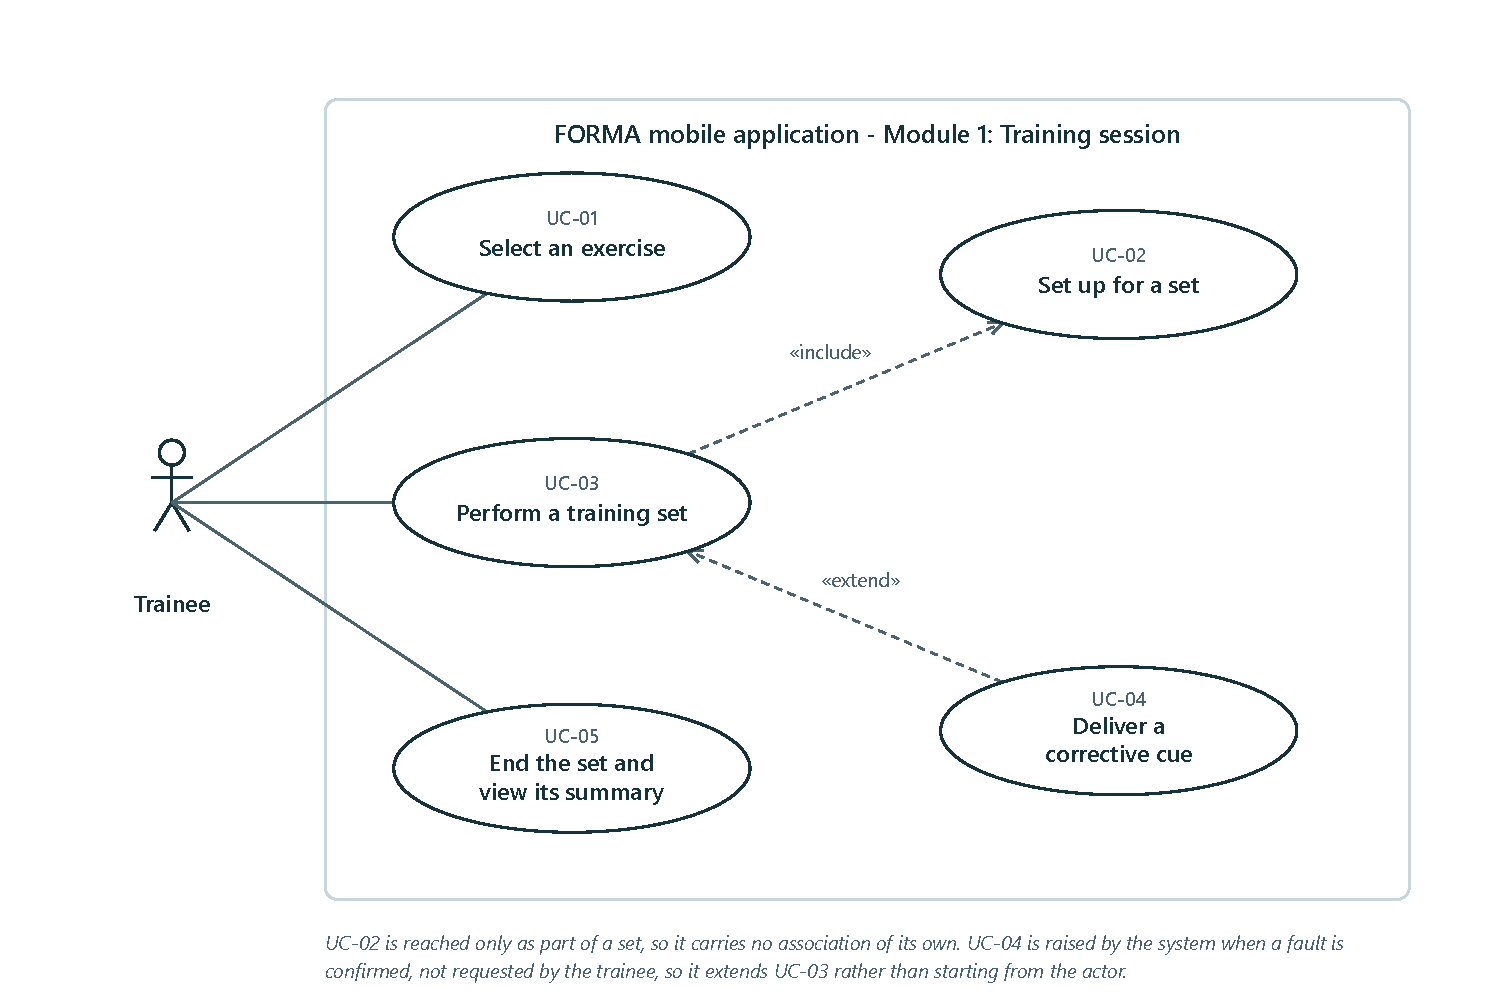
\includegraphics[width=\textwidth]{fig-3-1-use-case-module-1.pdf}
\caption[Use cases of Module 1, the training session]{Use cases of Module 1. The subject of the diagram is the mobile application, which in this module communicates with no other system at all.}
\label{fig:3.1}
\end{figure}

UC-03 is the central use case and the only one with a hard timing constraint. Two relationships carry meaning here and both are worth stating.

UC-02 is included rather than associated. Setting up happens every time a set is performed and never on its own. It is part of performing a set, not something the trainee does for its own sake. It does not gate the set: it shows the exercise, reports the framing and hands the decision to start to the trainee.

UC-04 extends UC-03 and has no actor association. A cue happens when a fault is confirmed and at no other time. That makes it conditional, which is what an extension is. The system raises it; the trainee does not ask for it. That is why no line reaches it from the actor.

\subsection{Module 2: history and the profile}
\label{sec:3.2.2}

\begin{figure}[htbp]
\centering
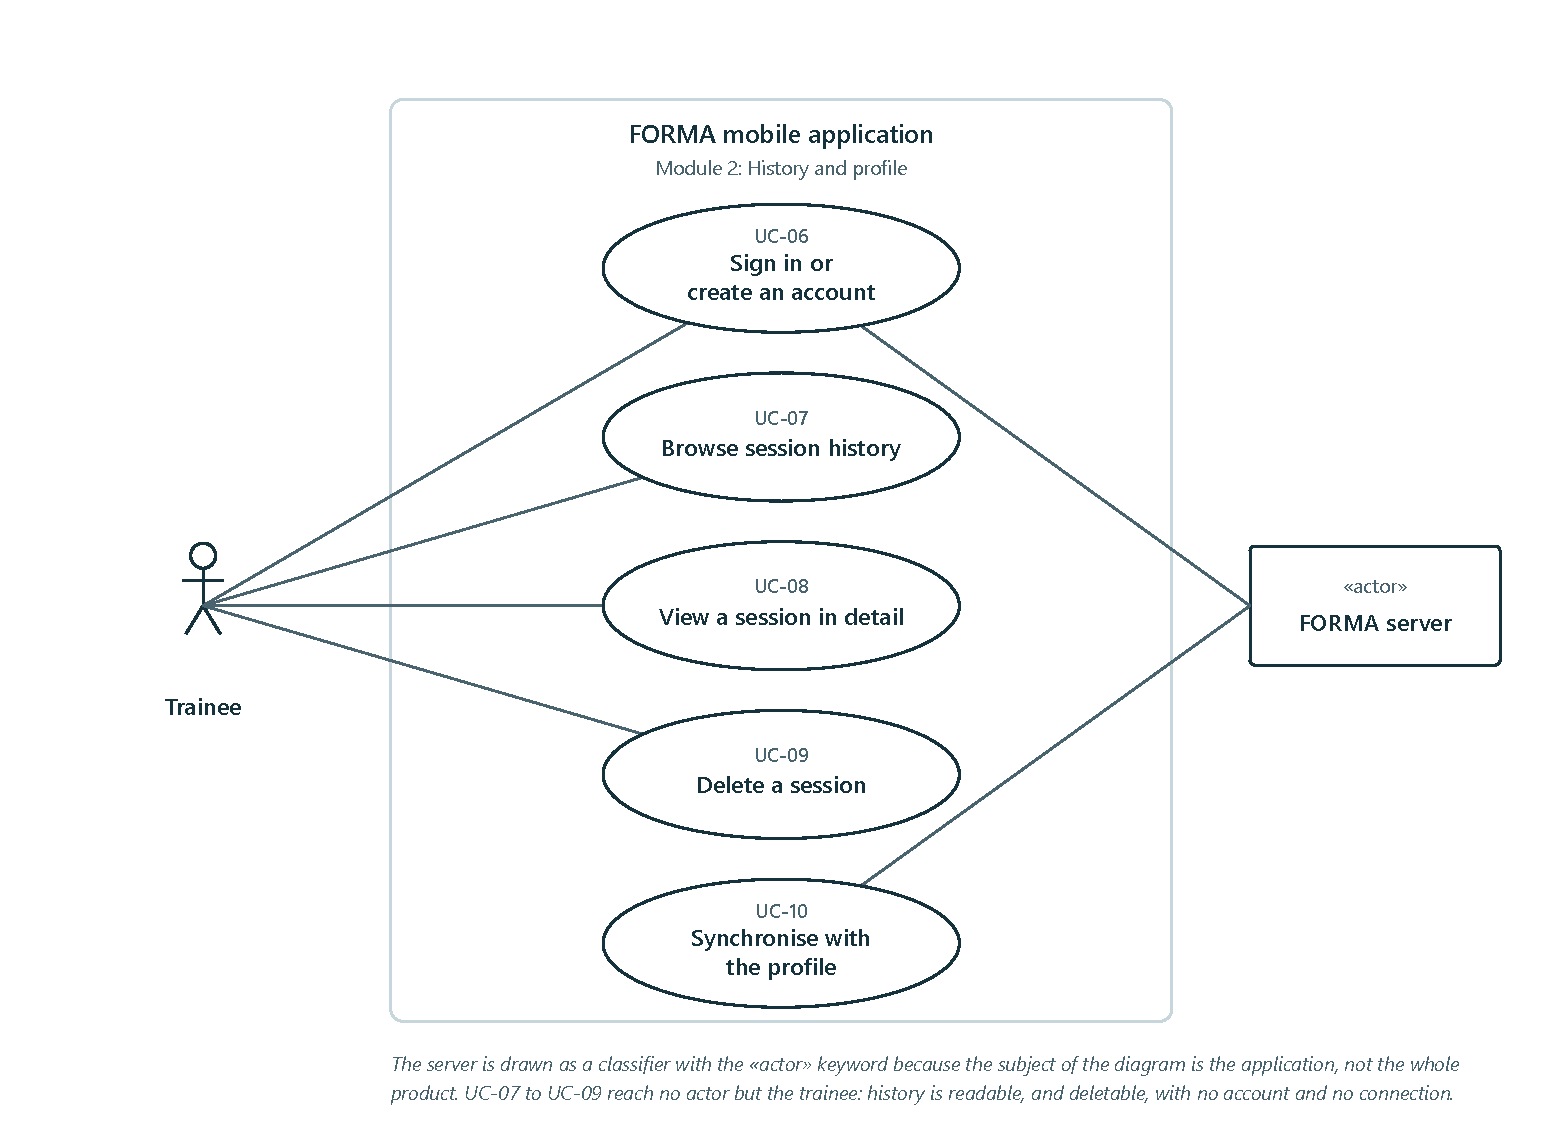
\includegraphics[width=\textwidth]{fig-3-2-use-case-module-2.pdf}
\caption[Use cases of Module 2, history and the profile]{Use cases of Module 2. Only two of the five reach the server, and the three the trainee uses most reach it not at all.}
\label{fig:3.2}
\end{figure}

A record held only on the device is lost with the device, and a trainee who changes phones after a year of training loses the year. That is what the profile is for.

UC-07, UC-08 and UC-09 connect to the trainee alone. Browsing the history, opening a session and deleting one all work with no account and no connection, because the device already holds the records it wrote. Signing in adds durability and a second device; it is not the price of using the product.

UC-10 is drawn with an association to the server and none to the trainee, because it is not something the user does. The application performs it when it is signed in and finds a connection, and the user's involvement ends at having signed in once.

\subsection{Scenario: UC-03, perform a training set}
\label{sec:3.2.3}

{\small
\setlength{\LTpre}{6pt}\setlength{\LTpost}{8pt}
\begin{longtable}{>{\raggedright\arraybackslash}p{\dimexpr 0.338\textwidth-2\tabcolsep\relax}>{\raggedright\arraybackslash}p{\dimexpr 0.662\textwidth-2\tabcolsep\relax}}
\caption{UC-03, perform a training set: actors, preconditions and postcondition}\\
\toprule
\endfirsthead
\endhead
\bottomrule
\endlastfoot
Actor & Trainee \\
Precondition & An exercise is selected and its specification is loaded \\
Postcondition & A completed set is recorded on the device \\
\end{longtable}
}

Main flow:

\begin{enumerate}
\item The trainee indicates that they are ready to begin.
\item The system shows how the exercise is performed: a diagram of the position the measurement is defined against, the camera placement the specification assumes, and what each fault will ask for. It is shown the first time an exercise is chosen and on request after that.
\item The system starts the camera and the pose pipeline and reports the framing conditions declared in the specification: whether the required landmarks are visible, whether the viewing angle is within tolerance, and whether the body occupies an acceptable part of the frame. When a condition fails it states the correction needed on screen and goes on reporting it. The trainee starts the set when they choose to.
\item The system announces the start of the set.
\item For each frame, the system computes the repetition driver declared in the specification and evaluates the fault conditions scoped to the current phase of the movement.
\item On a completed repetition, the count is incremented, and any fault the specification declares as a property of the repetition is decided at that boundary.
\item When a fault condition holds across the confirmation window and the trigger policy permits speech, the system extends into UC-04 and speaks one cue.
\item Steps 5 to 7 repeat until the trainee ends the set.
\item The system stops the pipeline and proceeds to UC-05.
\end{enumerate}

Alternate flows:

{\small
\setlength{\LTpre}{6pt}\setlength{\LTpost}{8pt}
\begin{longtable}{>{\raggedright\arraybackslash}p{\dimexpr 0.090\textwidth-2\tabcolsep\relax}>{\raggedright\arraybackslash}p{\dimexpr 0.411\textwidth-2\tabcolsep\relax}>{\raggedright\arraybackslash}p{\dimexpr 0.499\textwidth-2\tabcolsep\relax}}
\caption{UC-03 alternate flows: what the system does when a step cannot proceed}\\
\toprule
 & Condition & Behaviour \\
\midrule
\endfirsthead
\toprule
 & Condition & Behaviour \\
\midrule
\endhead
\bottomrule
\endfoot
\bottomrule
\endlastfoot
A1 & The trainee leaves the frame, or landmarks are lost & Counting is suspended and the system says so once. It resumes automatically. Repetitions during the gap are not counted, and the gap appears in the summary \\
A2 & Two faults hold within the same repetition & Both are recorded. The trigger policy selects at most one to speak \\
A3 & A confirmed fault has no authored cue & The fault is recorded and nothing is spoken. The summary reports it \\
A4 & The repetition driver is ambiguous, for example the trainee pauses mid-movement & No repetition is counted until the driver crosses its hysteresis bound \\
A5 & The sustained frame rate falls below the floor in NFR-P2 & The system says so, and the set is recorded as degraded rather than reported as an ordinary result \\
A6 & The application is interrupted, for example by an incoming call & The set ends and is recorded as incomplete, with the partial count preserved \\
\end{longtable}
}

Step 3 reports rather than refuses, and the reason is practical before it is philosophical. The trainee has to be at the phone to press start. A check performed before that measures the framing of somebody standing beside the camera, which is not the framing of the set. A gate placed there buys very little and costs the trainee a product that decides whether they are allowed to train. What camera placement does bound is what the assessment can see, so the condition is stated plainly and goes on being stated. A2, A3 and A5 share the principle: where the system has less information than it needs, it says so rather than producing an answer anyway.

\subsection{Scenario: UC-10, synchronise with the profile}
\label{sec:3.2.4}

{\small
\setlength{\LTpre}{6pt}\setlength{\LTpost}{8pt}
\begin{longtable}{>{\raggedright\arraybackslash}p{\dimexpr 0.313\textwidth-2\tabcolsep\relax}>{\raggedright\arraybackslash}p{\dimexpr 0.687\textwidth-2\tabcolsep\relax}}
\caption{UC-10, synchronise with the profile: actors, preconditions and postcondition}\\
\toprule
\endfirsthead
\endhead
\bottomrule
\endlastfoot
Actor & FORMA server, as a secondary actor. The application initiates \\
Precondition & The trainee is signed in \\
Postcondition & The device and the profile hold the same set of sessions \\
\end{longtable}
}

Main flow:

\begin{enumerate}
\item The application observes that a connection is available and that records exist which the profile has not acknowledged.
\item The application sends those records. Each carries the exercise, the specification version in force, the repetition count, the fault codes with their counts, and the timestamps. No frame and no image is sent, because none was ever kept.
\item The server writes each record under the user profile against an identifier generated on the device, so that a record already held is replaced rather than added a second time.
\item The application sends deletions made while offline, and the server removes the corresponding records.
\item The server returns records held in the profile that this device does not have.
\item The application marks the local records as acknowledged.
\end{enumerate}

Alternate flows:

{\small
\setlength{\LTpre}{6pt}\setlength{\LTpost}{8pt}
\begin{longtable}{>{\raggedright\arraybackslash}p{\dimexpr 0.090\textwidth-2\tabcolsep\relax}>{\raggedright\arraybackslash}p{\dimexpr 0.405\textwidth-2\tabcolsep\relax}>{\raggedright\arraybackslash}p{\dimexpr 0.505\textwidth-2\tabcolsep\relax}}
\caption{UC-10 alternate flows}\\
\toprule
 & Condition & Behaviour \\
\midrule
\endfirsthead
\toprule
 & Condition & Behaviour \\
\midrule
\endhead
\bottomrule
\endfoot
\bottomrule
\endlastfoot
B1 & The connection drops part way through & Records that were not acknowledged stay unacknowledged and are sent again later. Step 3 is keyed by identifier, so resending cannot duplicate \\
B2 & A session was deleted on one device and is still present in the profile & The deletion is applied. A record the user removed does not return \\
B3 & The trainee is not signed in & No synchronisation happens, and the device keeps a complete history of its own \\
\end{longtable}
}

B1 is the reason step 3 is written the way it is. Synchronisation over a mobile connection fails part way through as a matter of routine rather than as an exception, so the protocol has to be safe to repeat. Making the write replace rather than append costs nothing and removes the whole class of failure in which a retry doubles a user's training history.

\section{Functional Requirements}
\label{sec:3.3}

Each requirement is written so that it can be shown to hold or not to hold. The final column traces it to an objective from 1.3: O1 on-device perception, O2 movement assessment, O3 immediate spoken feedback, O4 the application, the server service and the user profile, O5 traceable fault definitions and a labelling protocol, O6 a labelled dataset and a testing procedure.

\subsection{Module 1: the training session}
\label{sec:3.3.1}

{\small
\setlength{\LTpre}{6pt}\setlength{\LTpost}{8pt}
\begin{longtable}{>{\raggedright\arraybackslash}p{\dimexpr 0.106\textwidth-2\tabcolsep\relax}>{\raggedright\arraybackslash}p{\dimexpr 0.797\textwidth-2\tabcolsep\relax}>{\raggedright\arraybackslash}p{\dimexpr 0.097\textwidth-2\tabcolsep\relax}}
\caption{Functional requirements for the training session}\\
\toprule
ID & Requirement & Serves \\
\midrule
\endfirsthead
\toprule
ID & Requirement & Serves \\
\midrule
\endhead
\bottomrule
\endfoot
\bottomrule
\endlastfoot
FR-01 & The trainee can select an exercise from those whose specification is loaded & O2 \\
FR-02 & The system evaluates camera framing before and during a set and states the correction needed when the framing is not usable, without preventing the set from starting & O1 \\
FR-03 & The system judges a repetition against the absolute criteria declared in the specification, with no measurement of the trainee taken beforehand & O2, O5 \\
FR-04 & The system estimates body pose from the camera feed in real time, entirely on the device & O1 \\
FR-05 & The system segments repetitions and maintains a live count for the current set & O2 \\
FR-06 & The system detects the technique faults declared in the active specification & O2, O5 \\
FR-07 & The system speaks a corrective cue, drawn from a bank of pre-authored lines, while the trainee is still performing the set & O3 \\
FR-08 & The system applies a trigger policy that governs when it speaks and when it stays silent & O3 \\
FR-09 & The trainee can end a set and see a summary of repetitions and faults & O2 \\
FR-10 & The system records the completed set on the device, whether or not a network is available & O4 \\
FR-28 & Before a set the system shows how the exercise is performed: the position the measurement is defined against, the camera placement the specification assumes, and what each fault asks for. It is shown the first time an exercise is chosen, can be dismissed for that exercise, and can be reopened from the set-up screen & O3, O5 \\
\end{longtable}
}

\subsection{Module 2: history and the profile}
\label{sec:3.3.2}

{\small
\setlength{\LTpre}{6pt}\setlength{\LTpost}{8pt}
\begin{longtable}{>{\raggedright\arraybackslash}p{\dimexpr 0.106\textwidth-2\tabcolsep\relax}>{\raggedright\arraybackslash}p{\dimexpr 0.797\textwidth-2\tabcolsep\relax}>{\raggedright\arraybackslash}p{\dimexpr 0.097\textwidth-2\tabcolsep\relax}}
\caption{Functional requirements for history and the profile}\\
\toprule
ID & Requirement & Serves \\
\midrule
\endfirsthead
\toprule
ID & Requirement & Serves \\
\midrule
\endhead
\bottomrule
\endfoot
\bottomrule
\endlastfoot
FR-11 & The trainee can create an account and sign in & O4 \\
FR-12 & The trainee can browse past sessions in reverse chronological order, with no account and no connection & O4 \\
FR-13 & The trainee can open a session and see, per set, the repetitions, the faults and their counts & O4 \\
FR-14 & The trainee can see, for any fault, its plain-language description, what to do differently next time, and the source its definition came from & O5 \\
FR-15 & The trainee can delete a session & O4 \\
FR-16 & When signed in and connected, the system synchronises locally recorded sessions to the user profile, and repeating a synchronisation does not duplicate a record & O4 \\
FR-17 & A deletion made while offline is applied to the profile at the next synchronisation, and the record does not return & O4 \\
FR-18 & Signing in on a device makes the profile's session history available on that device & O4 \\
\end{longtable}
}

\subsection{Cross-cutting}
\label{sec:3.3.3}

{\small
\setlength{\LTpre}{6pt}\setlength{\LTpost}{8pt}
\begin{longtable}{>{\raggedright\arraybackslash}p{\dimexpr 0.106\textwidth-2\tabcolsep\relax}>{\raggedright\arraybackslash}p{\dimexpr 0.797\textwidth-2\tabcolsep\relax}>{\raggedright\arraybackslash}p{\dimexpr 0.097\textwidth-2\tabcolsep\relax}}
\caption{Cross-cutting functional requirements}\\
\toprule
ID & Requirement & Serves \\
\midrule
\endfirsthead
\toprule
ID & Requirement & Serves \\
\midrule
\endhead
\bottomrule
\endfoot
\bottomrule
\endlastfoot
FR-19 & The system loads exercise definitions from specification files, with no change to application code & O2 \\
FR-20 & Every function in Module 1 operates with no network available & O1, O3 \\
FR-21 & No camera frame is written to storage, and no image data leaves the device & O1 \\
FR-22 & Only derived results leave the device: counts, fault codes, timestamps and specification versions & O1, O4 \\
FR-23 & A specification that fails validation is rejected when it is loaded, with the failure named, rather than loaded in part & O2 \\
FR-24 & Every fault a specification declares resolves to an audio asset, checked when the specification is loaded rather than discovered as silence during a set & O3 \\
FR-25 & Every fault a specification declares carries a provenance record & O5 \\
FR-26 & A session record stores the specification version in force when the set was performed, and the per-repetition detail behind its fault counts & O5, O6 \\
FR-27 & Where the system cannot support a result it says so instead of producing one. Loss of pose suspends counting and is announced, and a frame rate below the floor is reported & O6 \\
\end{longtable}
}

FR-03 replaced a requirement for a per-user calibration step. That step was removed from the design, for the reasons 4.5.1 gives, and the requirement went with it rather than being carried and missed. NFR-P6, which bounded how long the calibration could take, is gone for the same reason and leaves a gap in the numbering rather than renumbering requirements that other chapters cite.

The specification format cannot express a fault without a provenance record, so FR-25 is checked by the parser rather than resting on the author remembering it.

FR-22's list is exhaustive: if a field is not on it, it does not leave the device.

\section{Non-Functional Requirements}
\label{sec:3.4}

\subsection{Deriving the response-time requirement}
\label{sec:3.4.1}

The governing quantity is how long the system may take between a fault becoming present in the movement and the trainee hearing about it. Every other performance requirement in this chapter follows from it.

Three inputs go into it.

The first is the movement. A controlled bodyweight squat repetition takes two to three seconds, and the descent is roughly half of that. The derivation uses the faster end, one second of descent, because a requirement derived from the slower end would be satisfied by accident.

The second is what a cue is for. A cue exists to change the repetition it describes, which means it has to arrive while the trainee is still in the phase in which the fault occurred. A depth cue heard during the ascent is describing a descent that is over.

The third is that the larger share of that phase belongs to the trainee, not to the system. They have to hear a short phrase, recognise it, and begin to act on it, and that is not instantaneous.

From these, the rule the budget is built on: the system may consume at most a third of the phase in which the fault occurs, leaving two thirds to the person who has to respond. A third of a one-second descent is a little over 330 ms, so the requirement is set at 300 ms, which keeps a margin inside the derivation rather than spending it.

That total is then allocated across the stages between the fault and the sound.

{\small
\setlength{\LTpre}{6pt}\setlength{\LTpost}{8pt}
\begin{longtable}{>{\raggedright\arraybackslash}p{\dimexpr 0.434\textwidth-2\tabcolsep\relax}>{\raggedright\arraybackslash}p{\dimexpr 0.133\textwidth-2\tabcolsep\relax}>{\raggedright\arraybackslash}p{\dimexpr 0.433\textwidth-2\tabcolsep\relax}}
\caption{The response-time budget, allocated across the stages between fault and sound}\\
\toprule
Stage & Allocation & What it covers \\
\midrule
\endfirsthead
\toprule
Stage & Allocation & What it covers \\
\midrule
\endhead
\bottomrule
\endfoot
\bottomrule
\endlastfoot
Confirming that the fault is real & 140 ms & Three frame intervals. The reason for three is below \\
Camera capture to the frame reaching the application & 30 ms & One frame period at a conventional capture rate \\
Frame preparation & 15 ms & Format and geometry, before inference \\
Pose inference & 45 ms & One forward pass over one frame \\
Constraint evaluation & 5 ms & Arithmetic over a few dozen points \\
Cue selection & 5 ms & A table lookup and the trigger counters \\
Audio dispatch to the first audible sample & 60 ms & A pre-rendered asset, with no synthesis in the path \\
Total & 300 ms &  \\
\end{longtable}
}

Only the total is a requirement. The split is a planning allocation, and a stage that overruns is acceptable as long as another underruns, because what the trainee experiences is the sum.

Two things in that table need their own argument.

The confirmation window exists because a fault has to be seen more than once before it is worth speaking about. One frame is not evidence: a single noisy landmark can satisfy any threshold. Two frames are not much better, because a single outlier next to one true observation still carries the decision. Three is the smallest number for which no single sample is decisive, and because it is the smallest, it is also the cheapest in time.

The audio line is specified as the first audible sample rather than simply the first sample. Speech assets are commonly padded with silence at the front, and a file whose first sample is silent satisfies the loose wording while failing the requirement as meant, since the requirement exists so that the trainee can act on what they hear.

\textbf{The frame rate follows from the confirmation window.} Everything except confirmation is allocated 160 ms, which leaves 140 ms for three frame intervals. An interval of at most 46 ms is a frame rate of at least 21.4 frames per second, so the floor is 22 fps, the lowest whole rate that satisfies it.

\textbf{The requirement also constrains the design.} The work the table allocates to one frame, from capture to assessment, comes to 95 ms, which is more than twice the 46 ms interval the frame-rate floor demands. A pipeline that captured a frame, processed it to completion, and only then captured the next could not reach 22 fps at all. The budget is satisfiable only by a design in which capture and assessment overlap.

\subsection{Performance}
\label{sec:3.4.2}

{\footnotesize
\setlength{\LTpre}{6pt}\setlength{\LTpost}{8pt}
\begin{longtable}{>{\raggedright\arraybackslash}p{\dimexpr 0.125\textwidth-2\tabcolsep\relax}>{\raggedright\arraybackslash}p{\dimexpr 0.407\textwidth-2\tabcolsep\relax}>{\raggedright\arraybackslash}p{\dimexpr 0.146\textwidth-2\tabcolsep\relax}>{\raggedright\arraybackslash}p{\dimexpr 0.322\textwidth-2\tabcolsep\relax}}
\caption{Performance requirements}\\
\toprule
ID & Requirement & Target & How it is verified \\
\midrule
\endfirsthead
\toprule
ID & Requirement & Target & How it is verified \\
\midrule
\endhead
\bottomrule
\endfoot
\bottomrule
\endlastfoot
NFR-P1 & Fault onset to the first audible sample of the cue & 300 ms or less & Instrumented timestamps on the target device, over recorded sets \\
NFR-P2 & Sustained frame rate during a set & 22 fps or more & Benchmark run on the target device \\
NFR-P3 & Per-frame latency, from the frame reaching the application to its assessment being complete, 95th percentile & 65 ms or less & Benchmark run on the target device \\
NFR-P4 & The NFR-P2 floor holds for the whole of a session, not only at its start & Throughout ten minutes & One continuous ten-minute run \\
NFR-P5 & Cold start to a usable camera preview & 3 s or less & Repeated manual timing \\
\end{longtable}
}

NFR-P3 is a percentile rather than a mean. A mean hides exactly the behaviour that damages the product: a cue that arrives late on one repetition in twenty is a defect the trainee will notice and an average cannot show. The 65 ms figure is the sum of the stages the application itself controls: preparation, inference and evaluation. The requirement is that this allocation holds for nineteen frames in twenty, not just on the average frame.

NFR-P4 exists because the frame rate that matters is the one in the tenth minute. Any phone warms under sustained camera and inference load and throttles when it does, and a pipeline that is comfortable for thirty seconds and misses the floor by minute eight cannot support a ten-minute session. The requirement is that the floor holds throughout. It does not permit a percentage of decline, because a decline that stays above the floor costs the trainee nothing, and one that does not is a failure whatever its size.

\subsection{Accuracy and reliability}
\label{sec:3.4.3}

The system will miss some faults. It must not invent any. That asymmetry is a product decision before it is a numeric target.

A trainee corrected while they were performing correctly learns that the system is unreliable, and from that point every later cue is discounted, including the correct ones. A missed fault costs one uncorrected repetition. A false cue costs the trainee's confidence in the product, and that is not recovered within the session.

{\footnotesize
\setlength{\LTpre}{6pt}\setlength{\LTpost}{8pt}
\begin{longtable}{>{\raggedright\arraybackslash}p{\dimexpr 0.125\textwidth-2\tabcolsep\relax}>{\raggedright\arraybackslash}p{\dimexpr 0.342\textwidth-2\tabcolsep\relax}>{\raggedright\arraybackslash}p{\dimexpr 0.152\textwidth-2\tabcolsep\relax}>{\raggedright\arraybackslash}p{\dimexpr 0.381\textwidth-2\tabcolsep\relax}}
\caption{Accuracy and reliability requirements}\\
\toprule
ID & Requirement & Target & How it is verified \\
\midrule
\endfirsthead
\toprule
ID & Requirement & Target & How it is verified \\
\midrule
\endhead
\bottomrule
\endfoot
\bottomrule
\endlastfoot
NFR-A1 & Fault detection precision, per fault & 0.90 or more & The evaluation set confirmed by a certified trainer \\
NFR-A2 & Fault detection recall, per fault & 0.70 or more & The evaluation set confirmed by a certified trainer \\
NFR-A3 & Repetition count error, per set & 1 repetition or less & Labelled video \\
NFR-A4 & Identical landmark input produces identical output & Exact & Unit tests over recorded sequences, with no device in the loop \\
NFR-A5 & A session completes with no crash and no restart & Ten minutes continuous & One continuous ten-minute run \\
NFR-A6 & Loss of pose is handled explicitly rather than silently & Always & Scripted interruption tests \\
\end{longtable}
}

The gap between NFR-A1 and NFR-A2 is the requirement. The two figures are targets and either could be argued with, but the precision target being materially higher than the recall target is the asymmetry above expressed as a number, and that is not an accident of two separately chosen values.

NFR-A4 is what makes the assessment layer testable without a phone. Given fixed model weights, the same landmark sequence produces the same fault codes every time, so recorded sequences can be replayed as ordinary unit tests.

NFR-A6 concerns the common case rather than an edge case. A trainee steps out of frame, turns the wrong way, or is occluded by their own arm. The system suspends counting and says so; it does not keep reporting a count it cannot support.

\subsection{Privacy and data protection}
\label{sec:3.4.4}

The product's privacy claim is narrower than ``it works offline'' and stronger than a policy. The claim is that the video never leaves the phone, and it holds even though the application does use the network.

{\footnotesize
\setlength{\LTpre}{6pt}\setlength{\LTpost}{8pt}
\begin{longtable}{>{\raggedright\arraybackslash}p{\dimexpr 0.125\textwidth-2\tabcolsep\relax}>{\raggedright\arraybackslash}p{\dimexpr 0.424\textwidth-2\tabcolsep\relax}>{\raggedright\arraybackslash}p{\dimexpr 0.118\textwidth-2\tabcolsep\relax}>{\raggedright\arraybackslash}p{\dimexpr 0.333\textwidth-2\tabcolsep\relax}}
\caption{Privacy and data protection requirements}\\
\toprule
ID & Requirement & Target & How it is verified \\
\midrule
\endfirsthead
\toprule
ID & Requirement & Target & How it is verified \\
\midrule
\endhead
\bottomrule
\endfoot
\bottomrule
\endlastfoot
NFR-S1 & No camera frame or still image is written to storage at any point & Absolute & Code review, and an inspection of application storage after a session \\
NFR-S2 & No image data is transmitted. What leaves the device is derived: counts, fault codes, timestamps and specification versions & Absolute & Code review, and inspection of the request payloads \\
NFR-S3 & The assessment path requires no network. A set recorded offline is complete and nothing about it is deferred & Absolute & A full session with the network disabled \\
NFR-S4 & Session data is held in the application's own storage on the device, and under the signed-in profile on the server, and nowhere else & Absolute & Code review, and an inspection of the device after a session \\
NFR-S5 & Deleting a session removes it from the device at once, and from the profile at the next synchronisation & Absolute & Functional test, offline and online \\
\end{longtable}
}

An application that synchronises needs network access, and the operating system's permission model does not distinguish a number from an image once that access is granted. NFR-S2 is therefore verified by reading what the application sends rather than by what it is permitted to send, which is a weaker form of assurance than a structural one.

What does hold structurally is NFR-S1. A frame that was never written cannot later be uploaded, and the absence of any write path is visible to a reviewer reading the code rather than inferred from behaviour.

\textbf{The client asks for one permission, and that is checkable without reading any code.} \texttt{aapt dump \allowbreak{}permission\allowbreak{}s} on the built APK reports \texttt{CAMERA} and nothing else. Three further permissions reached the merged manifest at one point and were removed: the merger implies storage and phone-state access when any dependency declares a \texttt{target\allowbreak{}Sdk\allowbreak{}Version} below 4, which one transitive library does, and nothing in the application or that library calls an API they protect.

\textbf{NFR-S4 says the application's own storage rather than private storage, because the distinction matters.} Records are written to application-specific external storage, which belongs to this application, is removed when it is uninstalled, and has needed no permission since API 19. It is not the same as internal storage: on API 26 to 28 another application holding \texttt{READ\_\allowbreak{}EXTERNAL\_\allowbreak{}STORAGE} could read it, and only scoped storage from API 29 closes that. The move to internal storage waits. The measurement workflow this project runs on reads those files over \texttt{adb}.

\subsection{Usability}
\label{sec:3.4.5}

One constraint dominates this section: during the activity the product exists for, the trainee can neither look at the screen nor touch it. The camera faces them, so the display does not, and their hands are occupied by the movement.

{\footnotesize
\setlength{\LTpre}{6pt}\setlength{\LTpost}{8pt}
\begin{longtable}{>{\raggedright\arraybackslash}p{\dimexpr 0.125\textwidth-2\tabcolsep\relax}>{\raggedright\arraybackslash}p{\dimexpr 0.298\textwidth-2\tabcolsep\relax}>{\raggedright\arraybackslash}p{\dimexpr 0.348\textwidth-2\tabcolsep\relax}>{\raggedright\arraybackslash}p{\dimexpr 0.229\textwidth-2\tabcolsep\relax}}
\caption{Usability requirements}\\
\toprule
ID & Requirement & Target & How it is verified \\
\midrule
\endfirsthead
\toprule
ID & Requirement & Target & How it is verified \\
\midrule
\endhead
\bottomrule
\endfoot
\bottomrule
\endlastfoot
NFR-U1 & No interaction is required between the start and the end of a set & Absolute & Observed sessions \\
NFR-U2 & Every instruction given during a set is complete in audio alone & Absolute & Review of the cue bank and of the in-set prompts \\
NFR-U3 & A cue is a single imperative phrase & 5 words or fewer & Review of the cue bank \\
NFR-U4 & Cues spoken in one set & Within the ceiling the specification declares, which a hold may leave open & Trigger policy test \\
NFR-U5 & Cues spoken at the same time & Never more than one & Trigger policy test \\
NFR-U6 & Opening the application to the start of the first set & 60 s or less & Repeated manual timing \\
\end{longtable}
}

NFR-U4 is a trust requirement before it is a comfort requirement. A system that speaks continuously is experienced as criticism rather than coaching, and a trainee who feels criticised stops listening, which costs the product everything the other requirements bought.

The ceiling is declared per exercise rather than fixed here, because the two movement shapes pace themselves differently. A counting exercise supplies its own rhythm: the fault clears at the top of every repetition, which gives the trainee a moment to act, and both counting specifications cap a set at six. A hold supplies none of that. The position is held, the fault persists until the trainee changes something, and there is no repetition boundary to pace against, so the plank declares no ceiling and keeps correcting until the fault goes away.

\textbf{That is a deliberate exception and it is the most likely thing in this chapter to be wrong about a real person.} A trainee who sags for a full forty-five second hold and never corrects will hear the cue about twenty times. Whether that is coaching or nagging is a question for the trainee and for the trainers who review the fault set. It is recorded here as an open judgement.

NFR-U3 and NFR-U4 also interact with the budget in 3.4.1. A short imperative phrase occupies roughly a second of speech, so a system that spoke freely would be speaking over itself within a single set. The word limit keeps the cue inside the time the movement allows.

\subsection{Extensibility}
\label{sec:3.4.6}

{\footnotesize
\setlength{\LTpre}{6pt}\setlength{\LTpost}{8pt}
\begin{longtable}{>{\raggedright\arraybackslash}p{\dimexpr 0.125\textwidth-2\tabcolsep\relax}>{\raggedright\arraybackslash}p{\dimexpr 0.443\textwidth-2\tabcolsep\relax}>{\raggedright\arraybackslash}p{\dimexpr 0.118\textwidth-2\tabcolsep\relax}>{\raggedright\arraybackslash}p{\dimexpr 0.314\textwidth-2\tabcolsep\relax}}
\caption{Extensibility requirements}\\
\toprule
ID & Requirement & Target & How it is verified \\
\midrule
\endfirsthead
\toprule
ID & Requirement & Target & How it is verified \\
\midrule
\endhead
\bottomrule
\endfoot
\bottomrule
\endlastfoot
NFR-E1 & Adding an exercise within a supported movement category requires no change to application code & Absolute & The diff of the change that adds one \\
NFR-E2 & An exercise is defined by exactly one specification file and its audio assets & Absolute & File inventory for each exercise \\
NFR-E3 & A specification that fails validation is rejected at load, with the failure named & Absolute & Unit tests over deliberately malformed specifications \\
NFR-E4 & Every fault a specification declares carries a provenance record, enforced by the format rather than by convention & Absolute & Schema validation \\
\end{longtable}
}

NFR-E1 is the requirement O2 turns on, and the one most easily claimed without evidence. The verification is a diff: if adding an exercise touched application code, the requirement failed.

\section{Constraints and Assumptions}
\label{sec:3.5}

\subsection{Constraints}
\label{sec:3.5.1}

These are fixed from outside the requirements and are not negotiable within this phase.

{\small
\setlength{\LTpre}{6pt}\setlength{\LTpost}{8pt}
\begin{longtable}{>{\raggedright\arraybackslash}p{\dimexpr 0.090\textwidth-2\tabcolsep\relax}>{\raggedright\arraybackslash}p{\dimexpr 0.910\textwidth-2\tabcolsep\relax}}
\caption{Constraints the project works within}\\
\toprule
ID & Constraint \\
\midrule
\endfirsthead
\toprule
ID & Constraint \\
\midrule
\endhead
\bottomrule
\endfoot
\bottomrule
\endlastfoot
C1 & One target device, as 1.4.1 states. Nothing measured on it supports a claim about any other handset \\
C2 & One camera in one position. No second camera, no depth sensor and no wearable \\
C3 & Three exercises: the bodyweight squat, the push-up and the front plank \\
C4 & No medical, diagnostic or rehabilitative output, as 1.4.2 states. The system observes movement and cannot distinguish a technique fault from an existing injury \\
C5 & Every figure this project reports is either a measurement whose run is named at the point it appears, or a target. This chapter contains targets only \\
\end{longtable}
}

\subsection{Assumptions}
\label{sec:3.5.2}

These are taken to be true. Each one, if wrong, changes something above, and the consequence is stated so that a reader can judge the exposure.

{\small
\setlength{\LTpre}{6pt}\setlength{\LTpost}{8pt}
\begin{longtable}{>{\raggedright\arraybackslash}p{\dimexpr 0.090\textwidth-2\tabcolsep\relax}>{\raggedright\arraybackslash}p{\dimexpr 0.369\textwidth-2\tabcolsep\relax}>{\raggedright\arraybackslash}p{\dimexpr 0.541\textwidth-2\tabcolsep\relax}}
\caption{Assumptions, and what each one changes if it turns out to be wrong}\\
\toprule
ID & Assumption & If it is wrong \\
\midrule
\endfirsthead
\toprule
ID & Assumption & If it is wrong \\
\midrule
\endhead
\bottomrule
\endfoot
\bottomrule
\endlastfoot
AS1 & A controlled repetition takes two to three seconds, with the descent about half of it & A slower trainee makes NFR-P1 easier to meet. A trainee moving explosively shrinks the system's share below what the budget assumes, and the cue arrives too late to change that repetition, though still within the set \\
AS2 & A session involves up to ten minutes of continuous camera use & A longer session moves NFR-P4 beyond what the ten-minute run demonstrates, and thermal behaviour past that point is unknown rather than acceptable \\
AS3 & The trainee can hear the device, through headphones or in a quiet enough room & The feedback path is audio. If it cannot be heard, no requirement in 3.4 delivers anything \\
AS4 & The phone can be placed to the side at a distance that puts the whole body in frame & This is reported rather than assumed, which is what FR-02 is for. Where it cannot be satisfied the set still runs, and the faults that need the missing landmarks go unmeasured rather than being judged on a partial view \\
AS5 & One person is in frame & A second person in view is out of scope for this phase and is not handled \\
AS6 & A short spoken phrase occupies roughly a second & A longer cue overruns the window the movement allows, which is the constraint NFR-U3 exists to hold \\
\end{longtable}
}

\chapter{Design Decisions and Justification}
\label{chap:4}

\section{Platform and Target Device}
\label{sec:4.1}

A constraint rather than a decision, stated first because every figure in the chapter depends on it.

The platform is Android: the development environment is Windows and an iOS build needs a macOS toolchain that is not available. The device is the Samsung Galaxy Z Flip5 named in 1.4.1, read from the handset with \texttt{adb shell \allowbreak{}getprop} rather than from a specification sheet. It was not selected against alternatives. It is the handset this project had, which 3.5.1 records as C1, and every figure below describes it and no other.

An emulator is useful during development and is not a target, because it measures neither real camera behaviour nor thermal throttling, the two unknowns the measurement exists to resolve.

\section{Pose Estimation Engine}
\label{sec:4.2}

Pose estimation sets the ceiling for everything after it: a joint absent from the model's output cannot be observed by any rule downstream.

\textbf{Latency decides, and it decides twice.} NFR-P3 bounds the 95th percentile of the per-frame path at 65 ms, and NFR-P2 sets a frame-rate floor of 22 fps, which 3.4.1 derives from the confirmation window. The second reaches further, because that window is counted in frames rather than milliseconds, so every frame per second buys response time as well as a smoother signal.

\textbf{Licence is a product constraint rather than a formality.} A copyleft licence that propagates to the application is a decision taken now whether or not it is noticed now.

\textbf{Topology is headroom, not a requirement.} The COCO seventeen-keypoint layout stops at the ankle, with no heel and no toe, and all six faults this project retains are expressible in it. It eliminates nothing here, and 4.6 is what makes the headroom matter.

\subsection{Shortlisting on published evidence}
\label{sec:4.2.1}

{\footnotesize
\setlength{\LTpre}{6pt}\setlength{\LTpost}{8pt}
\begin{longtable}{>{\raggedright\arraybackslash}p{\dimexpr 0.170\textwidth-2\tabcolsep\relax}>{\raggedright\arraybackslash}p{\dimexpr 0.257\textwidth-2\tabcolsep\relax}>{\raggedright\arraybackslash}p{\dimexpr 0.242\textwidth-2\tabcolsep\relax}>{\raggedright\arraybackslash}p{\dimexpr 0.198\textwidth-2\tabcolsep\relax}>{\raggedright\arraybackslash}p{\dimexpr 0.133\textwidth-2\tabcolsep\relax}}
\caption{Pose engines shortlisted on published evidence}\\
\toprule
Engine & Topology & Licence & Android integration & Model swappable \\
\midrule
\endfirsthead
\toprule
Engine & Topology & Licence & Android integration & Model swappable \\
\midrule
\endhead
\bottomrule
\endfoot
\bottomrule
\endlastfoot
Media\allowbreak{}Pipe Pose Landmarker & 33 landmarks, heel and foot index included & Apache 2.0 & First-class Tasks API & Yes \\
MoveNet & 17, COCO & Apache 2.0 & TFLite, with a sample application & Yes \\
RTMPose & 17 COCO, 26 in the Halpe variant & Apache 2.0 & ncnn export plus glue code & Yes \\
YOLO-pose & 17, COCO & AGPL-3.0, or a paid commercial licence & Export path required & Yes \\
ML Kit Pose Detection & 33 landmarks & Proprietary, free to use & Lowest, through Play Services & No \\
\end{longtable}
}

Published performance figures exist for some of these and are not used to choose. The BlazePose figure is over 30 frames per second on a Pixel 2 (Bazarevsky et al., 2020)\cite{bazarevsky2020blazepose}, and the MoveNet figures are latency on a Pixel 5 (TensorFlow Blog, MoveNet, 2021)\cite{tensorflow2021movenet}. Neither device is the handset this project targets, so those figures establish feasibility, which 2.3.1 covers, and not a choice on this handset.

Three options fall on the table above. \textbf{YOLO-pose} carries a licensing risk and offers nothing over the survivors, so the risk buys nothing. \textbf{RTMPose} needs an ncnn export and glue, and the deployability of its 26-keypoint variant here is unverified: a research task standing where a dependency should be. \textbf{ML Kit} publishes no latency figures, no accuracy figures and no way to substitute the model, and a system whose claim is that its behaviour can be checked cannot rest its perception layer on one that publishes nothing about its own. It is kept as a fallback.

Nothing on the table separates MediaPipe from MoveNet, so deciding between them on inspection would be deciding on preference. Both were measured on the target device, in the same harness, in one run.

\subsection{How the engines were measured}
\label{sec:4.2.2}

Appendix A describes the instrument, lists every run and gives the caveats. Three points bear on the table below.

\textbf{The harness runs the engine, not the product.} It has no constraint evaluation, no trigger policy and no audio, so NFR-P1 cannot be obtained from it at all and the comparison against NFR-P3 is favourable to the pipeline by whatever the missing stages cost.

\textbf{The device was not cold.} Battery temperature climbed from 34.1 C at the start of the sweep to a peak of 39.0 C, so a configuration measured late began warmer than one measured early. Here that runs against the winner.

\textbf{An earlier sweep measured a client defect and is superseded.} It put frame preparation at 44 ms against an allocation of 15. That was not the engine: the analyzer was rotating each frame in software when the engine accepts the rotation as a parameter. Removing it cut median preparation to 10 ms on the identical MediaPipe Lite GPU configuration, left median inference at 50 ms against 52, and took its frame rate from 17.70 to 29.84. An engine comparison taken while a fixed per-frame tax dominated every row would have been a comparison of the tax.

\subsection{What the measurement says}
\label{sec:4.2.3}

{\tiny
\setlength{\LTpre}{6pt}\setlength{\LTpost}{8pt}
\begin{longtable}{>{\raggedright\arraybackslash}p{\dimexpr 0.136\textwidth-2\tabcolsep\relax}>{\raggedright\arraybackslash}p{\dimexpr 0.117\textwidth-2\tabcolsep\relax}>{\raggedright\arraybackslash}p{\dimexpr 0.098\textwidth-2\tabcolsep\relax}>{\raggedright\arraybackslash}p{\dimexpr 0.138\textwidth-2\tabcolsep\relax}>{\raggedright\arraybackslash}p{\dimexpr 0.152\textwidth-2\tabcolsep\relax}>{\raggedright\arraybackslash}p{\dimexpr 0.126\textwidth-2\tabcolsep\relax}>{\raggedright\arraybackslash}p{\dimexpr 0.136\textwidth-2\tabcolsep\relax}>{\raggedright\arraybackslash}p{\dimexpr 0.097\textwidth-2\tabcolsep\relax}}
\caption{The engine comparison as measured on the target device}\\
\toprule
Engine & Delegate & Frames per second & Inference, median & Preparation, median & Total, 95th percentile & Knee jitter & Battery at start \\
\midrule
\endfirsthead
\toprule
Engine & Delegate & Frames per second & Inference, median & Preparation, median & Total, 95th percentile & Knee jitter & Battery at start \\
\midrule
\endhead
\bottomrule
\endfoot
\bottomrule
\endlastfoot
Media\allowbreak{}Pipe Lite & CPU & 27.61 & 80 ms & 9 ms & 107 ms & not measured & 34.1 C \\
Media\allowbreak{}Pipe Lite & GPU & 29.84 & 50 ms & 10 ms & 71 ms & 0.00045 & 35.9 C \\
Media\allowbreak{}Pipe Full & CPU & 18.29 & 104 ms & 11 ms & 137 ms & 0.00040 & 36.9 C \\
Media\allowbreak{}Pipe Full & GPU & 29.85 & 55 ms & 11 ms & 76 ms & 0.00028 & 37.1 C \\
Media\allowbreak{}Pipe Heavy & CPU & 5.86 & 225 ms & 12 ms & 262 ms & 0.00045 & 37.7 C \\
Media\allowbreak{}Pipe Heavy & GPU & 23.99 & 91 ms & 11 ms & 124 ms & 0.00024 & 38.2 C \\
MoveNet Lightning & CPU & 26.89 & 20 ms & 7 ms & 36 ms & 0.00066 & 39.0 C \\
MoveNet Lightning & GPU & 29.57 & 13 ms & 7 ms & 27 ms & 0.00111 & 38.5 C \\
\end{longtable}
}

The deciding sweep, on the device in 4.1, in the order printed, 60 measured seconds each at 720 by 1280. Appendix A names the run and holds its data. Total is preparation plus inference for one frame, the quantity NFR-P3 bounds at 65 ms. Jitter is the mean frame-to-frame movement of the knee with the subject still, in normalised units, and measures how quiet the model is rather than how accurate it is.

\textbf{One row is not a result.} The harness recorded that the framing gate timed out on MediaPipe Lite CPU and that it ran without a confirmed subject, and its knee detection rate is zero. Its timing columns measure the engine on an empty scene; its landmark columns measure nothing. It is printed with the gap visible, and at 107 ms it misses NFR-P3 by 42 ms whatever was in front of the camera.

\textbf{Frame rate no longer separates the top of the table.} Four configurations sit between 26.89 and 29.85 fps, which is the camera's 30 fps ceiling rather than a property of any model. In the superseded sweep nothing reached it and frame rate was the discriminator; here it is saturated, and what matters is the latency headroom underneath.

\textbf{Two configurations meet NFR-P3 and both are MoveNet}, at 27 ms on the GPU and 36 ms on the CPU. The best MediaPipe configuration is Lite on the GPU at 71 ms, and Full, Heavy and the two CPU variants follow at 76, 124, 137 and 262.

\textbf{MediaPipe Lite on the GPU straddles the bound rather than failing it.} The same configuration and build returned 60 ms on a cold device in an earlier run, 71 ms at 35.9 C here, and 79 ms at 36.8 C immediately afterwards. The engine is not inconsistent; the device is warm. A configuration whose compliance depends on the handset being cold complies at the start of a session and not at minute ten, which is what NFR-P4 exists to catch. MoveNet on the GPU has 2.4 times the bound in hand, and it ran last at 38.5 C, warmer than every MediaPipe row, so the thermal confound favours the loser.

\textbf{What MoveNet gives up is jitter.} The knee moves 0.00111 of a normalised unit per frame with the subject still against 0.00045 for MediaPipe Lite on the GPU, making MoveNet the noisiest model in the table by 2.5 times. Two assumptions turn that into judgeable units and neither is firm: the metric is a straight-line distance in coordinates that 6.2.1 shows are not a length, giving 0.8 pixels horizontally and 1.4 vertically, and the angle conversion needs a femur length the record does not store, taken at 256 pixels. The result is roughly 0.3 degrees of knee angle per frame, an order of magnitude under the 6 and 10 degree thresholds it has to support, and that holds with both assumptions wrong by a factor of two.

\textbf{Decision. MoveNet Lightning, on the GPU delegate.} Over MoveNet on the CPU on latency headroom, 27 ms against 36, which leaves more of the handset free for the rest of the pipeline. Over every MediaPipe configuration because none meets the requirement on a warm device.

\subsection{The engine was checked before it was trusted}
\label{sec:4.2.4}

The adapter between the output tensor and the assessment layer is written by hand, and MoveNet emits each keypoint as row, column and score rather than x, y and score. Read in the obvious order, that transposes every landmark while leaving every value inside its valid range, which is a system that fails silently.

The check is agreement with the engine being replaced. Over four 60-second runs of a subject standing still, three on MoveNet and one on MediaPipe Lite on the GPU, every MoveNet knee median fell within 0.035 of frame width and 0.015 of frame height of where MediaPipe put the same joint, with left and right on the correct sides. A transposed axis would have moved a knee by several tenths. Appendix A names the four runs, and the medians are in their per-frame files.

This rules out a class of integration defect and nothing more. There is no ground truth in it, so both engines could be wrong together. The subject also stood between runs instead of holding one position, so part of the disagreement is the subject.

\subsection{What this run does not settle}
\label{sec:4.2.5}

\textbf{NFR-P4 is not answered by this sweep.} Sixty seconds cannot show a thermal limit that arrives in the ninth minute, and at the time this comparison was made the only ten-minute runs on record were on MediaPipe, before the preparation fix. 9.4.1 reports a ten-minute run on the configuration this sweep chose.

\textbf{The jitter has a known cost and it was paid once already.} The segmenter tests whether the rep driver has stopped moving in order to name the bottom of a movement, and that threshold had been set at 0.05 degrees per frame against MediaPipe. MoveNet's noise floor at the knee is six times that, so the test could never be satisfied and the phase it gates was never entered: a recorded set of ten deliberately shallow squats raised nothing at all. A threshold calibrated against one engine's noise is a hidden dependency on that engine, and swapping the engine exposed it where failure was silent.

\textbf{The jitter columns compare two scores that are not the same quantity.} The harness counts a knee as present at a fixed floor of 0.5, while MediaPipe reports a visibility and MoveNet a keypoint heatmap score; on the same standing pose the knee scored 0.986 under one and 0.761 under the other. Both cleared the floor standing, so the reading here holds, but it would not in a flexed position where MoveNet's score falls further.

\textbf{Nothing here measures angular accuracy.} Jitter is repeatability with the subject still, not correctness. The choice is supported on everything measured and untested on that axis, which is the position 4.5.4 records for the thresholds.

\textbf{The comparison is between two engines, not five.} The other three were eliminated in 4.2.1 on licence, integration cost and disclosure, none of which a benchmark would have changed.

\textbf{What would reverse it.} A ten-minute run showing MoveNet losing the frame-rate floor under sustained load, which would promote MediaPipe Lite on the GPU and make NFR-P3 unmeetable on this handset. Or the landmark noise proving to change a verdict on recorded sets, which reopens the decision with MediaPipe Full on the GPU at a cost of 49 ms of 95th-percentile latency.

\section{Client and Backend Stack}
\label{sec:4.3}

Three questions settled together because they are one argument: what the client is written in, what runs where, and what the server is for. The hot path is a per-frame pipeline sustained for minutes, and every abstraction between the camera and the pose engine costs a buffer copy or a serialisation step inside a loop that 3.4.1 shows has no room.

\subsection{Client framework}
\label{sec:4.3.1}

{\footnotesize
\setlength{\LTpre}{6pt}\setlength{\LTpost}{8pt}
\begin{longtable}{>{\raggedright\arraybackslash}p{\dimexpr 0.233\textwidth-2\tabcolsep\relax}>{\raggedright\arraybackslash}p{\dimexpr 0.217\textwidth-2\tabcolsep\relax}>{\raggedright\arraybackslash}p{\dimexpr 0.234\textwidth-2\tabcolsep\relax}>{\raggedright\arraybackslash}p{\dimexpr 0.176\textwidth-2\tabcolsep\relax}>{\raggedright\arraybackslash}p{\dimexpr 0.140\textwidth-2\tabcolsep\relax}}
\caption{Client frameworks compared}\\
\toprule
Criterion & Native Kotlin & Flutter & React Native & Unity \\
\midrule
\endfirsthead
\toprule
Criterion & Native Kotlin & Flutter & React Native & Unity \\
\midrule
\endhead
\bottomrule
\endfoot
\bottomrule
\endlastfoot
Direct camera frame access & CameraX, first class & Through a channel, a copy per frame & Through a native module & Indirect \\
TFLite support on Android & First-class, the reference runtime & Community bindings & Community bindings & Limited \\
Overhead inside the per-frame path & None & A bridge crossing per frame & A bridge crossing per frame & Engine overhead \\
Control of the GPU delegate & Direct & Indirect & Indirect & Indirect \\
Benefit from being cross-platform & Not applicable & Unrealised & Unrealised & Unrealised \\
Interface capability for this product & Sufficient, with Compose & Strong & Strong & More than needed \\
\end{longtable}
}

\textbf{Decision. Native Android in Kotlin: CameraX for capture, TFLite for pose, Jetpack Compose for the interface, and one JSON file per set for the local store.}

The cross-platform options are rejected on one sufficient ground. Their principal benefit is serving iOS, which 4.1 excluded, while their principal cost is a bridge crossing inside the one path with a hard deadline. That is not a trade-off; it is one side of a trade with nothing on the other.

\subsection{Where the computation runs}
\label{sec:4.3.2}

{\footnotesize
\setlength{\LTpre}{6pt}\setlength{\LTpost}{8pt}
\begin{longtable}{>{\raggedright\arraybackslash}p{\dimexpr 0.200\textwidth-2\tabcolsep\relax}>{\raggedright\arraybackslash}p{\dimexpr 0.104\textwidth-2\tabcolsep\relax}>{\raggedright\arraybackslash}p{\dimexpr 0.270\textwidth-2\tabcolsep\relax}>{\raggedright\arraybackslash}p{\dimexpr 0.184\textwidth-2\tabcolsep\relax}>{\raggedright\arraybackslash}p{\dimexpr 0.242\textwidth-2\tabcolsep\relax}}
\caption{Where the computation runs: four placements compared}\\
\toprule
Criterion & All on device & Pose on device, assessment on a server & Frames streamed to a server & On device, records synchronised \\
\midrule
\endfirsthead
\toprule
Criterion & All on device & Pose on device, assessment on a server & Frames streamed to a server & On device, records synchronised \\
\midrule
\endhead
\bottomrule
\endfoot
\bottomrule
\endlastfoot
Satisfies NFR-P1 & Yes & No, the network is in the loop & No & Yes, the network is never in the loop \\
Image data leaves the device & No & No, landmarks only & Yes & No \\
Works with no connectivity & Yes & No & No & Yes, fully \\
History survives the device & No & Partly & Yes & Yes \\
Running cost per user & None & Per session & High & Per synchronisation \\
Load on the handset & Highest & Lower & Lowest & Highest \\
\end{longtable}
}

The two middle options fail on the first row structurally rather than as a matter of tuning: a network round trip inside a 300 ms budget cannot be made reliable over mobile data, and NFR-S3 is lost with it. The first and last differ on one row only, and keeping everything local loses the history with the phone, so a trainee who changes handsets after a year loses the year and FR-18 does not hold.

\textbf{Decision. The live path runs entirely on the device. Session records synchronise to a server-side profile when a connection exists and the trainee is signed in.} The network is used between sets and after them, never during one, and what crosses it is the derived list in FR-22 and nothing else.

\subsection{The server}
\label{sec:4.3.3}

The phase 1 server has one job: hold the profile and the session history, and reconcile them with a device that may have been offline for a week.

\textbf{Decision. A single FastAPI service in Python over SQLite.} The workload that follows this phase is language-model orchestration, retrieval and a safety test suite, which is where the Python ecosystem is strongest, so choosing it now costs nothing and avoids a rewrite at the boundary.

\textbf{What this costs.} The whole compute load sits on the handset, which is the thermal risk 4.1 recorded, and nothing in this phase provides remote diagnostics, so a failure on a user's device cannot be investigated remotely.

\textbf{What would reverse it.} iOS entering scope. Or the handset proving unable to carry the load within its thermal envelope, which would force assessment onto the server and reopen 4.4 with it.

\section{Immediate Feedback Path}
\label{sec:4.4}

The product claim in 1.2 is a correction that arrives inside the repetition. 3.4.1 turns that into 300 ms from fault to first audible sample, of which 60 ms is allocated to getting sound out of the device.

A language model cannot fit that allocation.

{\small
\setlength{\LTpre}{6pt}\setlength{\LTpost}{8pt}
\begin{longtable}{>{\raggedright\arraybackslash}p{\dimexpr 0.381\textwidth-2\tabcolsep\relax}>{\raggedright\arraybackslash}p{\dimexpr 0.210\textwidth-2\tabcolsep\relax}>{\raggedright\arraybackslash}p{\dimexpr 0.409\textwidth-2\tabcolsep\relax}}
\caption{The cost assumed for each stage of the immediate feedback path}\\
\toprule
Stage & Assumed cost & Basis \\
\midrule
\endfirsthead
\toprule
Stage & Assumed cost & Basis \\
\midrule
\endhead
\bottomrule
\endfoot
\bottomrule
\endlastfoot
Network round trip & 50 to 300 ms & Mobile data, variable, occasionally much worse \\
Time to first token & 200 to 800 ms & A hosted model, typical range \\
Generation to the end of a short utterance & 200 to 600 ms & Streamed \\
Synthesis and the start of playback & 200 to 500 ms & Cloud or on-device speech \\
Total & roughly 0.65 to 2.2 s &  \\
\end{longtable}
}

\textbf{None of these is a measurement.} They are assumptions, recorded so the reasoning can be inspected, as 3.5.1 C5 requires. The argument does not depend on their precision: the optimistic end consumes most of a repetition and the pessimistic end exceeds it entirely.

A second force has nothing to do with time. A generated utterance is not fixed in advance, so nothing guarantees the wording stays inside what the system can support, and for a product whose claim is that every cue traces to a published criterion, free generation in the live path contradicts the claim.

{\footnotesize
\setlength{\LTpre}{6pt}\setlength{\LTpost}{8pt}
\begin{longtable}{>{\raggedright\arraybackslash}p{\dimexpr 0.238\textwidth-2\tabcolsep\relax}>{\raggedright\arraybackslash}p{\dimexpr 0.131\textwidth-2\tabcolsep\relax}>{\raggedright\arraybackslash}p{\dimexpr 0.197\textwidth-2\tabcolsep\relax}>{\raggedright\arraybackslash}p{\dimexpr 0.185\textwidth-2\tabcolsep\relax}>{\raggedright\arraybackslash}p{\dimexpr 0.249\textwidth-2\tabcolsep\relax}}
\caption{Four ways to produce a spoken cue, compared}\\
\toprule
Criterion & Hosted language model & On-device language model & Pre-authored cue bank & Template plus synthesis at playback \\
\midrule
\endfirsthead
\toprule
Criterion & Hosted language model & On-device language model & Pre-authored cue bank & Template plus synthesis at playback \\
\midrule
\endhead
\bottomrule
\endfoot
\bottomrule
\endlastfoot
Worst-case fault to audio & Fails the allocation & Unknown, likely marginal & Bounded: a lookup and playback & Bounded by synthesis, longer than a lookup \\
Wording fixed in advance & No & No & Yes & Yes \\
Works with no network & No & Yes & Yes & Yes \\
Traceable to the fault taxonomy & Weak & Weak & By construction & Yes \\
Can say something outside its competence & Yes & Yes & No & No \\
Cost in the live path & Moderate & High, competes with pose inference & Negligible & Low \\
Cost to add a cue & None & None & Author and render one clip & Write one string \\
Adapts its phrasing to the user & Yes & Yes & No & No \\
\end{longtable}
}

The on-device model competes for the scarcest resource, which 4.1 records as the thermal risk, and synthesis at playback puts a variable cost inside a 60 ms allocation for no gain over a clip rendered once.

\textbf{Decision. A bank of pre-authored cues with pre-rendered audio, keyed by a discrete fault code. No language model takes part in the live path.}

The system is two-tier by design: the reflex tier fires on a confirmed fault and is a dictionary lookup and a cached clip, while the deliberative tier belongs to the second phase, runs between sets and has no hard deadline. With no network call, no generation and no synthesis in the live path, the allocation is met by construction rather than by optimisation.

\subsection{What a pre-rendered bank turned out to cost, and what it caught}
\label{sec:4.4.1}

Rendering the bank exposed a defect in the wording of the requirement. The synthesiser pads every utterance with silence before the first word, measured at 95 to 111 ms across the eight cues the bank held at the time. A file whose first sample is silent satisfies a requirement written as time to the first sample and fails the same requirement written as time to the first audible sample, and the difference is roughly a third of the whole budget, hidden inside a binary asset where no test would have found it. The lead-in is now cut when the bank is generated, keeping 8 ms so playback does not begin mid-waveform, and 3.4.1 specifies the audible sample for this reason.

\textbf{What this costs.} What the system says during a set is fixed when the cue is authored, with no adaptation to the trainee inside the repetition, and the audio ships in the bundle.

\textbf{What it buys, beyond the latency.} The complete set of sentences the system can ever say during a set is finite and reviewable before release. This was not the reason for the decision.

\textbf{What would reverse it.} Measurement showing an on-device model produces first audio inside the allocation with output constrained to the taxonomy. Or measurement showing even the cached path misses the allocation, which would force the trigger policy to fire earlier in the movement.

\section{Movement Assessment Approach}
\label{sec:4.5}

The assessment layer takes a stream of landmarks per frame, and 4.4 fixes its output: a discrete fault code from a closed set, plus a repetition count. A design emitting only a continuous quality score cannot key the lookup.

Four forces. \textbf{There is no labelled training data and no budget to produce it}, where a supervised classifier needs hundreds to thousands of labelled examples per fault per exercise. \textbf{Every cue must trace to a documented reason}, which is O5: a rule states its reason in its own text, a classifier states a probability. \textbf{The live path shares silicon with pose estimation}, which 4.1 flags as the scarce resource. And, cutting against the choice that follows, \textbf{a geometric rule is not free of data}: a depth rule needs a number to compare against, so the difference between the options is one of quantity, not of kind.

{\footnotesize
\setlength{\LTpre}{6pt}\setlength{\LTpost}{8pt}
\begin{longtable}{>{\raggedright\arraybackslash}p{\dimexpr 0.183\textwidth-2\tabcolsep\relax}>{\raggedright\arraybackslash}p{\dimexpr 0.186\textwidth-2\tabcolsep\relax}>{\raggedright\arraybackslash}p{\dimexpr 0.167\textwidth-2\tabcolsep\relax}>{\raggedright\arraybackslash}p{\dimexpr 0.217\textwidth-2\tabcolsep\relax}>{\raggedright\arraybackslash}p{\dimexpr 0.247\textwidth-2\tabcolsep\relax}}
\caption{Three approaches to movement assessment, compared}\\
\toprule
Criterion & Learned classifier over sequences & Declared geometric constraints & Hybrid: rules segment, a model classifies & Self-supervised, with a small supervised head \\
\midrule
\endfirsthead
\toprule
Criterion & Learned classifier over sequences & Declared geometric constraints & Hybrid: rules segment, a model classifies & Self-supervised, with a small supervised head \\
\midrule
\endhead
\bottomrule
\endfoot
\bottomrule
\endlastfoot
Labelled data required & Hundreds to thousands per fault & Tens of clips to set a threshold & High & Moderate, and expert-labelled \\
Available to this project & No & Yes & No & No \\
States why it fired & No, a probability & Yes, the violated constraint & Partly & No \\
Traceable to the taxonomy & Weak & By construction & Partly & Weak \\
Cost in the live path & Model inference per repetition & Arithmetic per frame & Model inference & Model inference \\
Deterministic and unit-testable & No & Yes & Partly & No \\
Cost of a new exercise & Retraining, and new labels & Authoring a specification & Retraining & Retraining \\
Handles subtle or compound faults & Better & Only what the geometry shows & Better & Best \\
Published precedent & Common & Pose Trainer, in 2.3.2 & Common & Fitness-AQA, in 2.3.2 \\
\end{longtable}
}

The second row decides it. Three options are stronger on the last row and all three are unavailable, because each needs a labelled corpus that does not exist here. Choosing one would mean either inventing labels or not evaluating the result.

\textbf{Decision. Movement assessment is geometric constraints over landmark trajectories, declared per exercise, with absolute thresholds that the system states and the user is measured against.}

\subsection{Where the standard comes from, since the user does not supply it}
\label{sec:4.5.1}

The alternative is a per-user reference measured before the first set, and this project built one before removing it. It answers a real objection: a trainee whose ankle mobility does not permit a full squat will be told to go deeper on every repetition by a system holding one number for everybody, and 3.4.3 records that a cue the user cannot act on is the most damaging failure this product has.

It is answered in the wrong place, for three reasons in order of weight.

\textbf{A product that asks the user what correct looks like has inverted its own premise.} The purpose in 1.1 is that the system knows what a correct repetition is and the user does not. A calibration step grades the user against their own demonstration, so a wrong demonstration becomes the standard and is confirmed on every set afterwards. The failure is silent and it is worst for exactly the users the product exists for.

\textbf{The published sources give absolute criteria}, so the calibration was discarding evidence the project already had. The Functional Movement Screen defines adequate squat depth as the femur below horizontal, a statement about the body and not about a particular body. Implemented literally, that is the hip landmark at or below the knee landmark.

\textbf{A fixed criterion removes a class of invented number.} A threshold expressed as an offset from a calibration needs both the procedure and the offset, and the offset has no source.

The objection the calibration was built for remains. The containment is not a softer threshold. It is a different response: a trainee who cannot reach the position should be told once, as an observation about mobility, instead of being cued every repetition. That path is specified and not built, and 9.5 records it as outstanding.

\subsection{A criterion is not a tolerance, and the difference is measured}
\label{sec:4.5.2}

A threshold of exactly zero would have the system speak about differences it cannot resolve. Ten squats performed at a deliberately constant depth gave a standard deviation of 0.0107 at the deepest point of each repetition and a range of 0.0163 either side of its centre. At zero, those ten split six passes to four faults, which is the measurement's own noise reported as a difference in the trainee's form.

The threshold is set 0.0209 below the criterion, at which all ten pass. The direction is the one 3.4.3 requires, since a false positive costs more than a missed fault. In degrees of femur angle that is about six, a conversion needing a femur length the recording does not store and which was taken at 256 pixels. \textbf{The threshold itself is in recorded units and does not depend on that assumption.}

Two further things this number is not. It is not from a source, and the specification records its threshold source as empty rather than citing the FMS for a tolerance the FMS does not give. And it mixes the trainee's variation between repetitions with the measurement's noise on an identical position, which this procedure cannot separate.

The same procedure sets the two hip thresholds in the push-up and the plank; 6.4.2 gives those distributions. The principle is that where a published criterion exists it is implemented directly, where a tolerance is needed it is measured and labelled as measured, and where neither exists the number is marked provisional in the file carrying it.

\subsection{Three things authoring the rules changed}
\label{sec:4.5.3}

\textbf{A published criterion can be a better design than the one it authorises.} Forward lean was first written as an absolute 45 degrees, which is wrong in a way worth recording: lean in a bodyweight squat is set largely by femur-to-torso proportion and ankle mobility, neither under the trainee's control, so a fixed angle fires constantly on a long-femured trainee squatting correctly and never on a short-limbed one genuinely over-pitching. The Functional Movement Screen compares the upper torso to the tibia within the same frame, which adapts to the body without asking the body anything.

\textbf{Each repetition has to be judged on its own, and the obvious implementation does not do that.} A fault evaluated over a set naturally tracks the most violating value seen so far, which is right for a deviation that can appear at any moment and wrong for one describing a repetition as a whole. A trainee who squats shallow five times and then once slightly deeper, still above the line, has performed six faulty repetitions; a running extreme reports the deepest and clears the rest. The format therefore distinguishes a fault judged continuously from one judged once per repetition, the second decided from samples collected within that repetition and discarded at its boundary.

\textbf{The declared camera view and the observable fault set are one decision rather than two.} A measurement taken along the axis the camera looks down is not available at any accuracy. Knee valgus is a frontal measurement while the squat declares a side view, where the two knees project to nearly the same point; the engine still returns the occluded side, but it is an inference, and a threshold on an inference fires at random. The fault was removed rather than approximated, as was push-up elbow flare, and both exclusions are recorded in the specification files themselves.

\subsection{What this approach cannot do}
\label{sec:4.5.4}

\textbf{The thresholds rest on one subject and one session.} Every source located establishes that a deviation is a fault and gives an observable condition for it; none gives the quantity at which the fault begins. The tolerances were measured on the author, performing the fault on purpose, in a single session per exercise. A deliberate fault is larger than one appearing under fatigue, so every detection rate derived from those recordings is an upper bound. The format records the taxonomy source and the threshold source as separate fields, and the threshold field is empty for every fault in the three files.

\textbf{The fault set has not been reviewed by a certified trainer.} The protocol is in 10.4: a trainer labels recorded sets without seeing the system's output or the author's own labels, and what the trainers set is what the report reports.

\textbf{Only geometrically observable faults can be detected.} Tempo, control and bracing are outside this method, and 2.2 shows they are outside the whole category rather than outside this choice alone.

\textbf{A trainee who cannot reach the standard is told so on every repetition}, which is the cost of removing the calibration and is not yet contained.

\textbf{Compound faults are not modelled.} Two simultaneous faults produce two codes, and the trigger policy decides which is spoken.

\textbf{What would reverse it.} An expert-labelled corpus becoming available, making the self-supervised option viable for faults the rules cannot separate. Or rules failing to separate a named fault from correct execution on recorded clips, which would require that fault to be removed with the removal stated rather than approximated.

\section{Exercise Extensibility Mechanism}
\label{sec:4.6}

O2 commits the system to adding an exercise without hand-written rules, and 2.4 is why it matters: no surveyed product discloses how an exercise is added at all. If a reviewer asks how the third exercise was added and the answer involves writing a class, the claim fails in public.

{\footnotesize
\setlength{\LTpre}{6pt}\setlength{\LTpost}{8pt}
\begin{longtable}{>{\raggedright\arraybackslash}p{\dimexpr 0.254\textwidth-2\tabcolsep\relax}>{\raggedright\arraybackslash}p{\dimexpr 0.193\textwidth-2\tabcolsep\relax}>{\raggedright\arraybackslash}p{\dimexpr 0.184\textwidth-2\tabcolsep\relax}>{\raggedright\arraybackslash}p{\dimexpr 0.216\textwidth-2\tabcolsep\relax}>{\raggedright\arraybackslash}p{\dimexpr 0.153\textwidth-2\tabcolsep\relax}}
\caption{Four extensibility mechanisms, compared}\\
\toprule
Criterion & A class per exercise & A declarative specification & An embedded scripting language & A model per exercise \\
\midrule
\endfirsthead
\toprule
Criterion & A class per exercise & A declarative specification & An embedded scripting language & A model per exercise \\
\midrule
\endhead
\bottomrule
\endfoot
\bottomrule
\endlastfoot
Adding an exercise requires code & Yes & No & Yes, script code & No, but it requires data \\
Readable by a non-programmer & No & Yes & No & No \\
Reviewable against the taxonomy & Hard, the logic is scattered & Yes, one file per exercise & Partly & No \\
Testable with no device & Partly & Yes, data in, codes out & Partly & No \\
Expressiveness & Unlimited & Bounded & High & High \\
Risk of divergence between exercises & High, each author improvises & Low, the schema constrains & Moderate & Not applicable \\
Available to this project & Yes & Yes & Yes & No, it needs labels \\
\end{longtable}
}

A class per exercise is what the category appears to do and is the thing O2 exists to avoid. A scripting language buys expressiveness this phase does not need and gives up reviewability.

\textbf{Decision. An exercise is added by authoring one declarative specification file. A single generic evaluator executes it, and the evaluator is the only code.}

{\small
\setlength{\LTpre}{6pt}\setlength{\LTpost}{8pt}
\begin{longtable}{>{\raggedright\arraybackslash}p{\dimexpr 0.253\textwidth-2\tabcolsep\relax}>{\raggedright\arraybackslash}p{\dimexpr 0.747\textwidth-2\tabcolsep\relax}}
\caption{What a specification file declares, block by block}\\
\toprule
Block & Contents \\
\midrule
\endfirsthead
\toprule
Block & Contents \\
\midrule
\endhead
\bottomrule
\endfoot
\bottomrule
\endlastfoot
\texttt{landmarks} & Which landmarks this exercise depends on \\
\texttt{rep\_\allowbreak{}driver} & One scalar signal, how it is extracted, and hysteresis bounds for segmentation \\
\texttt{phases} & Named intervals over that signal \\
\texttt{faults} & Per fault: a code, whether it is judged every frame or once per repetition, the phases it is scoped to, the constraint, the threshold, and the provenance of that threshold \\
\texttt{excluded\_\allowbreak{}faults} & Faults considered and not implemented, each with its reason, so an absence is visible as a decision rather than an oversight \\
\texttt{cues} & Fault code to audio asset, keyed by language \\
\texttt{trigger} & Confidence floor, confirmation window, per-set rate limit \\
\texttt{framing} & The camera placement the exercise assumes, used by the pre-set check \\
\end{longtable}
}

The provenance field is not decoration. Putting it in the schema means a specification cannot be authored without answering where its numbers came from. It is also the only field an author can fill badly without the evaluator noticing, which is why the trainer review is what closes it.

\subsection{The claim, stated at the size it survives}
\label{sec:4.6.1}

{\small
\setlength{\LTpre}{6pt}\setlength{\LTpost}{8pt}
\begin{longtable}{>{\raggedright\arraybackslash}p{\dimexpr 0.249\textwidth-2\tabcolsep\relax}>{\raggedright\arraybackslash}p{\dimexpr 0.416\textwidth-2\tabcolsep\relax}>{\raggedright\arraybackslash}p{\dimexpr 0.335\textwidth-2\tabcolsep\relax}}
\caption{What each exercise beyond the first cost the evaluator}\\
\toprule
Exercise & New measurement function & Other evaluator feature \\
\midrule
\endfirsthead
\toprule
Exercise & New measurement function & Other evaluator feature \\
\midrule
\endhead
\bottomrule
\endfoot
\bottomrule
\endlastfoot
Bodyweight squat & the initial vocabulary & none \\
Push-up & \texttt{signed\_\allowbreak{}offset\_\allowbreak{}from\_\allowbreak{}line} & none \\
Plank & none & \texttt{reports:\allowbreak{} duration} \\
\end{longtable}
}

\texttt{signed\_\allowbreak{}offset\_\allowbreak{}from\_\allowbreak{}line} was needed because hip sag and hip pike are opposite deviations of the same body line, take opposite cues, and cannot be separated by the interior hip angle, which falls below 180 degrees for both. \texttt{reports:\allowbreak{} duration} was needed because a plank's result is seconds, and reporting one repetition for a ninety-second hold would be true and useless.

A third feature came later and not from a new exercise. The per-repetition evaluation mode in 4.5.3 was written to correct the squat after a recorded set showed the original mode reporting the wrong verdict. It is counted because it changed both the evaluator and the schema, and it is a different kind of cost: the other two were the price of reaching a new movement, this was the price of getting the first one right.

The claim is therefore stated as:

\begin{quoteblock}
Adding an exercise requires no change to application code once the measurement vocabulary it needs, and the movement category it belongs to, are supported. The three exercises in this phase required two evaluator features between them: one measurement function and one scoring mode. A fourth exercise in either category requires neither.
\end{quoteblock}

The ceiling was predicted and met where predicted: a movement needing state beyond the declared phases was recorded in advance as out of reach until the evaluator gained a feature, and the plank cost exactly one feature for that reason. What makes the claim worth anything is that the vocabulary converged. The plank was authored after the push-up, for an unrelated fault, and reached \texttt{signed\_\allowbreak{}offset\_\allowbreak{}from\_\allowbreak{}line} independently. A format requiring a new function per exercise is a scripting language with extra steps; one shared function across two exercises is the first evidence that this one is not. The evaluator carries eight measurement functions, of which the three specifications use five, and it holds no branch on any exercise name.

\textbf{What this costs.} No code does not mean no work. A new exercise still needs clips to set its thresholds, an authored and rendered cue per fault, a framing definition and validation.

\textbf{What would reverse it.} A fault proving inexpressible as a declared constraint, which would force a scripting escape hatch or a narrower claim. Or the evaluator accumulating exercise-specific branches, which would mean the class-per-exercise option had arrived through the back door.

\section{How These Decisions Depend on One Another}
\label{sec:4.7}

\begin{figure}[htbp]
\centering
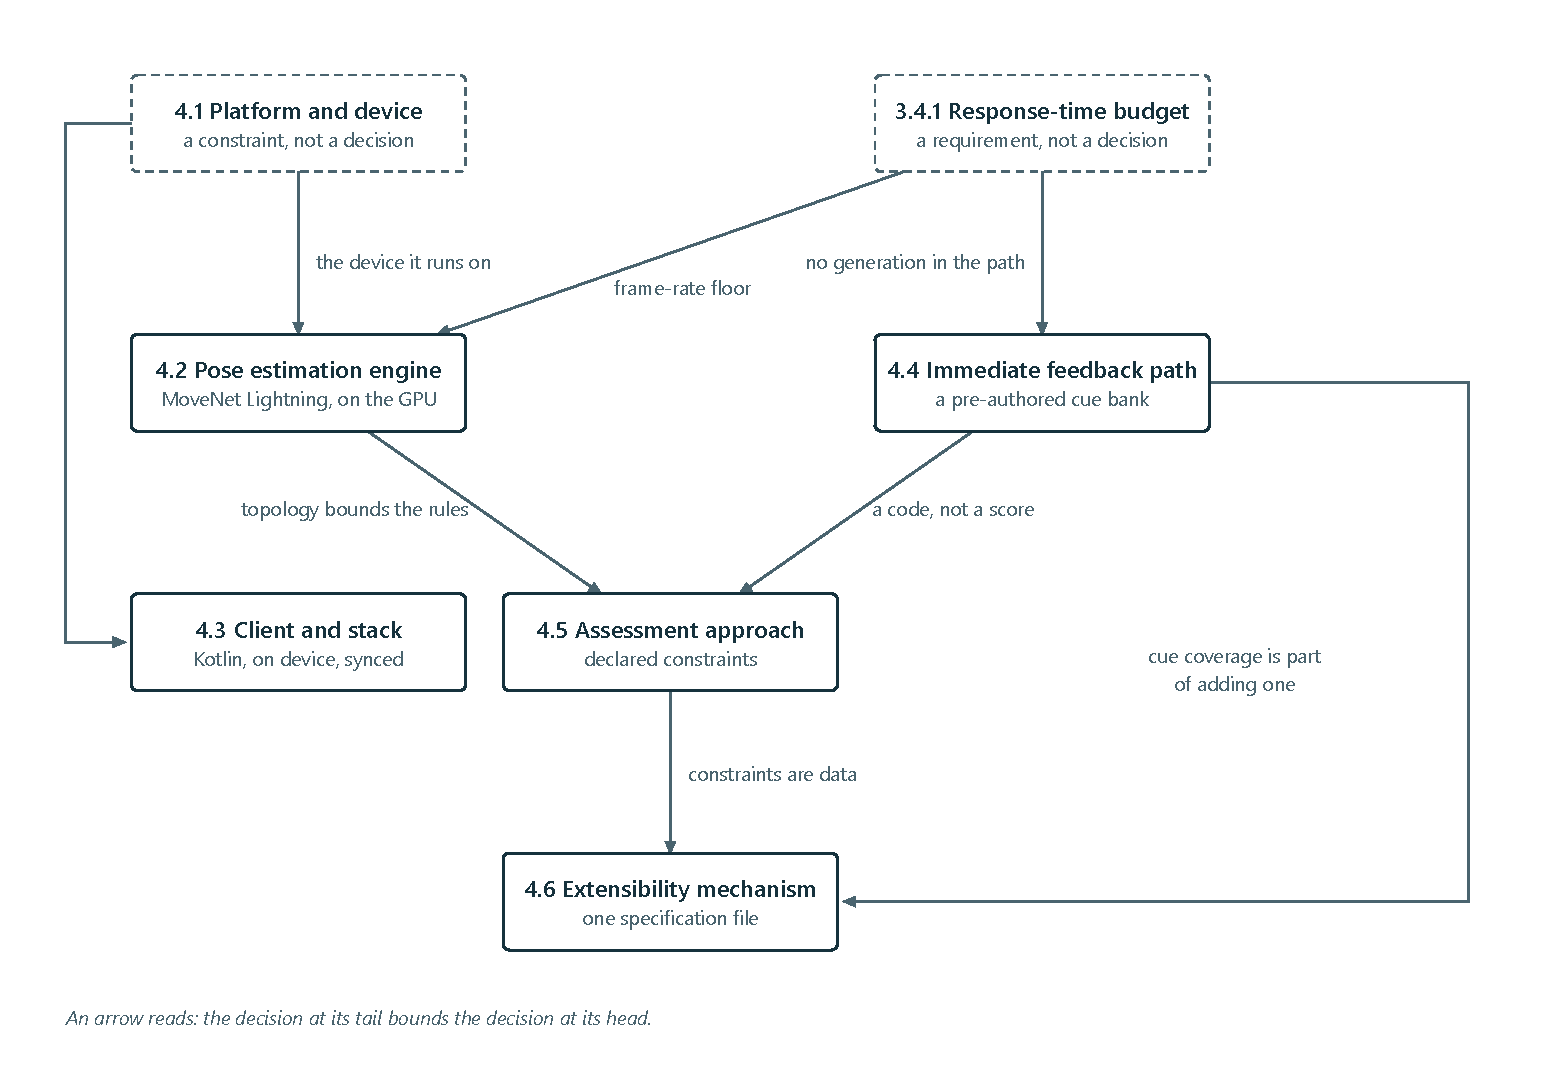
\includegraphics[width=\textwidth]{fig-4-1-decision-dependencies.pdf}
\caption[How the six design decisions constrain one another]{What constrains what. Dashed boxes are not decisions: one is a requirement and one is a constraint, and the chapter is ordered so that nothing is argued before the thing that bounds it.}
\label{fig:4.1}
\end{figure}

Two roots are not decisions. The response-time budget derived in 3.4.1 removes a language model from the live path in 4.4 and sets the frame-rate floor the engine is measured against in 4.2, and the handset in 4.1 is what every figure in the chapter is a figure about.

Three dependencies run in the direction a reader would not expect.

\textbf{The feedback path constrains the assessment layer rather than consuming whatever it produces.} Because the cue is a lookup on a discrete code, the assessment layer has to classify rather than score. A design emitting a continuous quality value would be reasonable in isolation and unusable here.

\textbf{The engine bounds the extensibility claim.} The format declares the landmarks an exercise depends on, so the set of exercises that can ever be declared is bounded by what the engine emits. The engine chosen in 4.2 stops at the ankle, so a future exercise whose fault needs the heel or the toe is not a specification away; it is an engine away.

\textbf{The engine's noise reaches the thresholds, which the arrows do not show.} A measurement noisier than the quantity being decided cannot support a threshold on it, so the number in 4.5.2 is a property of the engine in 4.2 as much as of the movement. 4.2.5 records the one place where that dependency was left implicit and failed silently.

\chapter{System Architecture}
\label{chap:5}

\section{Architectural Overview}
\label{sec:5.1}

\begin{figure}[htbp]
\centering
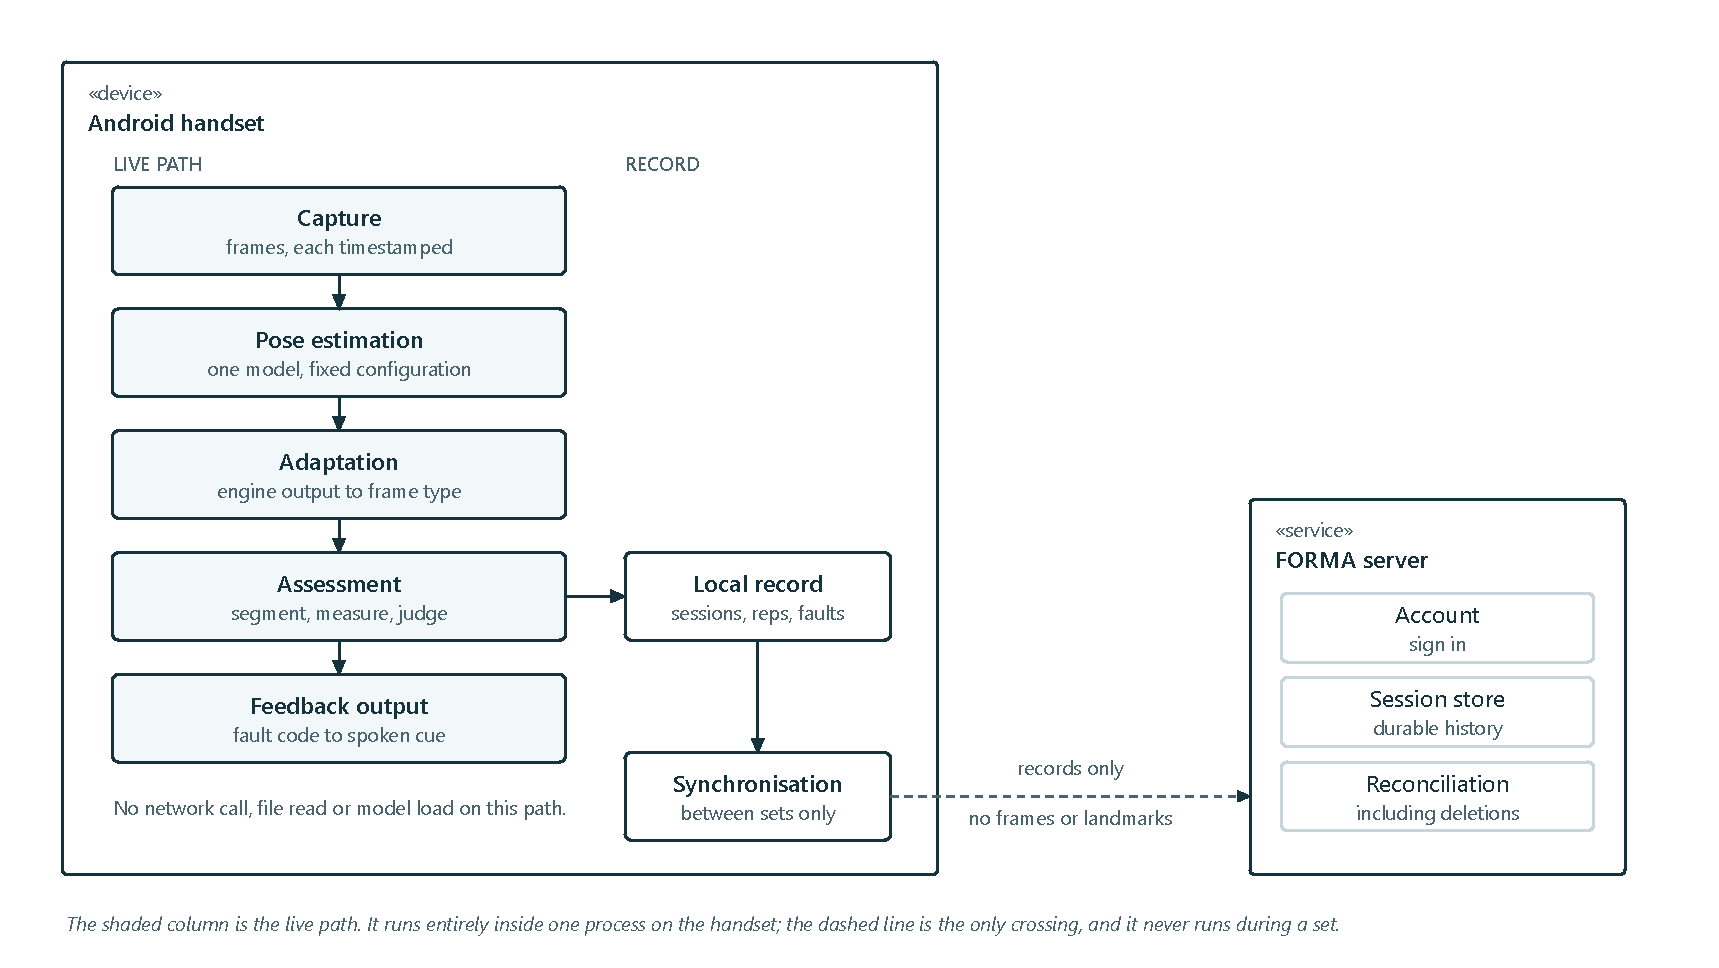
\includegraphics[width=\textwidth]{fig-5-1-architecture.pdf}
\caption[The two deployable parts and the one path with a deadline]{The shaded column is the live path. It runs entirely inside one process on the handset; the dashed line is the only crossing, and it carries records rather than movement.}
\label{fig:5.1}
\end{figure}

The system has two deployable parts and one property worth protecting.

The handset carries the whole of what happens during a set: the camera, the pose model, the assessment layer, and the sound. The server holds the account and the session history. Between them runs a single boundary that is crossed only between sets, and only by derived records.

The property being protected is the one 3.4.1 derives: 300 ms from a fault appearing in the movement to the trainee hearing about it. Everything in the arrangement above follows from refusing to put anything in that path that cannot be bounded. There is no network call on it, no file read, no model load, and no step whose duration depends on anything outside the process.

Two consequences follow, and both are deliberate.

\textbf{A set is complete without a network.} The trainee can train with the phone in aeroplane mode and lose nothing: the count, the faults, the cues and the record are all produced locally. Synchronisation adds durability across devices and is not the price of using the product.

\textbf{The video never exists as a file.} Frames are read from the camera, passed to the model, and released. No frame is written to storage at any point. That makes NFR-S1 a structural claim and not a policy. A reviewer can establish it by reading the code for a write path and finding none.

\section{Layers and Responsibilities}
\label{sec:5.2}

Four layers. Each one is defined as much by what it is forbidden to know as by what it does, because that is what keeps the evaluator testable without a device.

{\small
\setlength{\LTpre}{6pt}\setlength{\LTpost}{8pt}
\begin{longtable}{>{\raggedright\arraybackslash}p{\dimexpr 0.161\textwidth-2\tabcolsep\relax}>{\raggedright\arraybackslash}p{\dimexpr 0.493\textwidth-2\tabcolsep\relax}>{\raggedright\arraybackslash}p{\dimexpr 0.346\textwidth-2\tabcolsep\relax}}
\caption{The layers, what each owns, and what each is not allowed to know}\\
\toprule
Layer & Owns & Must not know \\
\midrule
\endfirsthead
\toprule
Layer & Owns & Must not know \\
\midrule
\endhead
\bottomrule
\endfoot
\bottomrule
\endlastfoot
Perception & Camera frames, the pose model, the output tensor & What an exercise is \\
Adaptation & Model output to the assessment layer's frame type & What the model is \\
Assessment & Segmentation, measurement, verdicts, the trigger policy & That Android exists \\
Presentation & The screen, the spoken cue, the session record & How a verdict was reached \\
\end{longtable}
}

\textbf{Perception has no vocabulary for exercise.} It produces seventeen points with scores, at whatever rate the camera and the delegate allow. It does not know that a squat exists, and swapping the model changes nothing above it.

\textbf{Adaptation is the only layer that knows both sides.} It converts the model's output tensor into the assessment layer's frame type: undoing the letterbox, applying the presence floor, and mapping index to landmark name. 4.2.4 records what this layer costs when it is wrong, which is why it has a layer of its own rather than being folded into either neighbour.

\textbf{Assessment is pure Kotlin with no Android dependency at all.} This is the load-bearing constraint in the whole arrangement. It takes a frame of named landmarks and a timestamp, and returns a phase, a count and a verdict. Because it imports nothing from the platform, a recorded landmark sequence can be replayed through it as an ordinary unit test, which is what makes NFR-A4 checkable and what 10.2 is built on.

\textbf{Presentation owns everything the trainee experiences} and none of the reasoning behind it. It receives a fault code and plays the clip that code names. It cannot compute a verdict and has no access to the geometry, so a change to how a fault is decided cannot reach the interface by accident.

\section{Deployment View}
\label{sec:5.3}

{\footnotesize
\setlength{\LTpre}{6pt}\setlength{\LTpost}{8pt}
\begin{longtable}{>{\raggedright\arraybackslash}p{\dimexpr 0.090\textwidth-2\tabcolsep\relax}>{\raggedright\arraybackslash}p{\dimexpr 0.134\textwidth-2\tabcolsep\relax}>{\raggedright\arraybackslash}p{\dimexpr 0.415\textwidth-2\tabcolsep\relax}>{\raggedright\arraybackslash}p{\dimexpr 0.361\textwidth-2\tabcolsep\relax}}
\caption{Where each part runs, what it holds, and how it is reached}\\
\toprule
 & Runs on & Holds & Reached \\
\midrule
\endfirsthead
\toprule
 & Runs on & Holds & Reached \\
\midrule
\endhead
\bottomrule
\endfoot
\bottomrule
\endlastfoot
Client & The handset & The specifications, the model, the cue bank, the local record & Always \\
Server & A single service & Accounts and the session history & Between sets, when signed in and connected \\
\end{longtable}
}

The client is self-contained. The three specification files, the model and every audio clip ship inside the application bundle, so a first run needs no download and a set can begin seconds after install. Nothing is fetched at runtime.

The server has one job, which 4.3.3 settles: hold the profile and reconcile it with a device that may have been offline for a week. It is deliberately small. It does no pose estimation, no assessment and no scoring, and it never receives an image.

\textbf{What crosses the boundary is the list in FR-22 and nothing else.} Counts, fault codes, timestamps and the specification version in force when the set was performed. The last of those is what lets a record be read correctly later: a fault code means what the specification of that version said it meant, and a record that did not carry its version would become uninterpretable the first time a threshold moved.

\section{Module Structure}
\label{sec:5.4}

Two Gradle modules, and the dependency runs one way.

{\small
\setlength{\LTpre}{6pt}\setlength{\LTpost}{8pt}
\begin{longtable}{>{\raggedright\arraybackslash}p{\dimexpr 0.174\textwidth-2\tabcolsep\relax}>{\raggedright\arraybackslash}p{\dimexpr 0.364\textwidth-2\tabcolsep\relax}>{\raggedright\arraybackslash}p{\dimexpr 0.462\textwidth-2\tabcolsep\relax}}
\caption{The two modules, and the dependency that runs one way between them}\\
\toprule
Module & Depends on & Contains \\
\midrule
\endfirsthead
\toprule
Module & Depends on & Contains \\
\midrule
\endhead
\bottomrule
\endfoot
\bottomrule
\endlastfoot
\texttt{assessment} & kotlinx-serialization only & The specification model, the segmenter, the measurement vocabulary, the evaluator, the trigger policy \\
\texttt{app} & \texttt{assessment}, Android, CameraX, TFLite, Compose & Camera, model, adapter, interface, audio, storage \\
\end{longtable}
}

\textbf{\texttt{assessment} has no Android dependency, and this is enforced rather than intended.} It is a plain Kotlin library. If someone adds an Android import to it, the module stops compiling, so the boundary cannot erode quietly through a convenient import.

Three things follow from it. The assessment layer runs on a desktop JVM, so its tests need no emulator and no device, and they run in seconds as part of an ordinary build. The same code runs unchanged under the offline replay harness in 9.3, which is what allows a recorded video to be scored by exactly the logic that runs on the phone. And the layer most likely to be reused in the second phase is the one with the fewest dependencies.

The module's tests load \textbf{the real specification files} from \texttt{docs/\allowbreak{}specs} rather than copies of them. A specification edited into an invalid state fails the build, which is the only arrangement under which the schema rules stay true of the files that actually ship.

\section{Data Flow}
\label{sec:5.5}

\subsection{The path of one frame}
\label{sec:5.5.1}

\begin{enumerate}
\item \textbf{CameraX delivers a frame} in the analyzer's own thread, with a timestamp taken at capture rather than at arrival.
\item \textbf{The adapter prepares it}: rotate to upright, letterbox into the square the model expects so the aspect ratio survives, hand the buffer over.
\item \textbf{The model returns seventeen keypoints}, each with a score. Points below the presence floor are dropped rather than passed on weak.
\item \textbf{The segmenter updates}: the driver is measured, smoothed, and compared against its hysteresis bounds, producing a phase and, at a boundary, a completed repetition.
\item \textbf{The evaluator judges.} Continuous faults are tested against the frames of their declared phases; per-repetition faults contribute a sample and are decided only at the closing boundary.
\item \textbf{The trigger policy decides whether to speak}, and usually does not.
\item \textbf{A cue plays}, as a clip already in memory.
\end{enumerate}

A frame can leave this path at any of several points, and leaving it is normal. No pose, a landmark below the visibility floor, a phase the fault is not scoped to, a streak too short to confirm, a confidence below the floor, a cue too soon after the last one. Each is a different reason for silence, and 6.5 covers what the trainee is told in each case.

\subsection{A frame that arrives while the engine is busy is dropped}
\label{sec:5.5.2}

The analyzer holds a single flag. If a frame arrives while the previous one is still in the model, the new frame is released immediately and never enters the pipeline.

The alternative is a queue, and a queue is wrong here in a way that gets worse the longer the set runs. Frames arrive at a fixed rate; if the pipeline is slower than that rate for even a short period, a queue grows and every frame in it is older than the movement it describes. The trainee would be corrected about a repetition finished several seconds earlier, and the lag would never recover within the set.

Dropping keeps every frame that is assessed current. The cost is that the effective frame rate is whatever the pipeline can sustain rather than whatever the camera offers, which is exactly the quantity NFR-P2 bounds and 4.2.3 measures.

\subsection{Why the frame rate is a floor rather than a preference}
\label{sec:5.5.3}

A dropped frame is not only a lost measurement. The confirmation window in 3.4.1 is counted in frames, so the frame rate sets how long confirmation takes in wall-clock time.

At 30 fps, three frames of confirmation cost 100 ms. At the 22 fps floor they cost 136 ms. At 15 fps they would cost 200 ms, which is two thirds of the entire response budget spent before the cue is even selected.

This is why frame rate appears in the engine decision twice over, and why 4.2 treats it as reaching further than its own column suggests. Every frame per second buys smoothness in the signal and response time in the cue.

\subsection{What crosses the boundary, and when}
\label{sec:5.5.4}

A set produces one record, written locally when the set ends.

{\small
\setlength{\LTpre}{6pt}\setlength{\LTpost}{8pt}
\begin{longtable}{>{\raggedright\arraybackslash}p{\dimexpr 0.445\textwidth-2\tabcolsep\relax}>{\raggedright\arraybackslash}p{\dimexpr 0.555\textwidth-2\tabcolsep\relax}}
\caption{The fields of a set record, and why each one is kept}\\
\toprule
Field & Why it is kept \\
\midrule
\endfirsthead
\toprule
Field & Why it is kept \\
\midrule
\endhead
\bottomrule
\endfoot
\bottomrule
\endlastfoot
Exercise and specification version & A fault code means what that version said it meant \\
Repetitions, or hold duration & The result the trainee asked for \\
Fault codes with counts & What was detected \\
Per-repetition detail & Which repetitions carried which verdict, and the value behind each \\
Cues spoken & What the trainee actually heard, which is not the same as what was detected \\
Timestamps & Ordering, and the elapsed time of the set \\
\end{longtable}
}

The per-repetition detail is worth its space. A count of faults answers how many; it does not answer which repetitions, or how close the others came to the same verdict. The record stores the value behind every repetition, whether or not it raised anything, so a later reader can tell a repetition that was comfortably correct from one that passed by a hair.

\textbf{Cues spoken is recorded separately from faults raised}, because the two differ by design. The trigger policy suppresses, and a set where six faults were detected and two were spoken is the policy working rather than the detector failing. Reporting only one of the two numbers would hide which.

Synchronisation sends these records and nothing else. No frame, no landmark, and no derived geometry. The server cannot reconstruct the movement from what it holds, which is the point.

\chapter{Movement Assessment Design}
\label{chap:6}

\section{From Exercise to Specification}
\label{sec:6.1}

An exercise is one JSON file. A single evaluator executes it, and the evaluator holds no branch on any exercise name.

{\small
\setlength{\LTpre}{6pt}\setlength{\LTpost}{8pt}
\begin{longtable}{>{\raggedright\arraybackslash}p{\dimexpr 0.253\textwidth-2\tabcolsep\relax}>{\raggedright\arraybackslash}p{\dimexpr 0.747\textwidth-2\tabcolsep\relax}}
\caption{What each block of a specification declares}\\
\toprule
Block & What it declares \\
\midrule
\endfirsthead
\toprule
Block & What it declares \\
\midrule
\endhead
\bottomrule
\endfoot
\bottomrule
\endlastfoot
\texttt{landmarks} & The points this exercise depends on. Eight for the squat, ten for the plank, twelve for the push-up \\
\texttt{framing} & The camera placement the exercise assumes, which landmarks the measurements need, and the reminders the set-up screen shows \\
\texttt{rep\_\allowbreak{}driver} & One scalar signal, how it is extracted, how it is smoothed, and the two bounds that segment it \\
\texttt{phases} & The named intervals over that signal \\
\texttt{faults} & Per fault: a code, whether it is judged every frame or once per repetition, the phases it is scoped to, the constraint, the threshold, and where that threshold came from \\
\texttt{excluded\_\allowbreak{}faults} & Deviations considered and not implemented, each with its reason \\
\texttt{cues} & Fault code to audio asset, keyed by language \\
\texttt{trigger} & Confidence floor, rate limits, and the order faults are spoken in \\
\end{longtable}
}

The evaluator reads the file, validates it, and refuses to load one that fails validation rather than loading the parts that parse. A specification that names a landmark the engine does not emit, a measurement function that does not exist, or a fault with no cue is rejected at load with the failure named, which is FR-23 and NFR-E3.

Three things are worth drawing out about the shape of the format.

\textbf{The provenance field is not optional.} A fault cannot be expressed without one, so the question of where a number came from is answered when the file is written rather than when someone asks. The field separates the taxonomy source from the threshold source, and those two are in very different states, which 6.4.2 sets out.

\textbf{Exclusions are recorded in the file that defines the exercise.} A reviewer asking why the squat does not detect knees caving in finds the answer beside the faults it does detect, with the reason, what was tried instead, and what would make it expressible later. An absence with no reason beside it is indistinguishable from an oversight.

\textbf{Nothing in the format describes an algorithm.} It declares what to measure and what to compare it against. How a measurement is computed belongs to the evaluator's vocabulary, which is shared across exercises and tested independently of all of them.

\section{Landmarks and Measurements}
\label{sec:6.2}

The engine emits the COCO seventeen-keypoint layout. Twelve of the seventeen are used; the five face points are returned on every frame and no rule reads them.

{\small
\setlength{\LTpre}{6pt}\setlength{\LTpost}{8pt}
\begin{longtable}{>{\raggedright\arraybackslash}p{\dimexpr 0.275\textwidth-2\tabcolsep\relax}>{\raggedright\arraybackslash}p{\dimexpr 0.725\textwidth-2\tabcolsep\relax}}
\caption{The landmarks each exercise depends on}\\
\toprule
 & Points used \\
\midrule
\endfirsthead
\toprule
 & Points used \\
\midrule
\endhead
\bottomrule
\endfoot
\bottomrule
\endlastfoot
Squat & shoulder, hip, knee, ankle, both sides \\
Push-up & shoulder, elbow, wrist, hip, knee, ankle, both sides \\
Plank & shoulder, elbow, hip, knee, ankle, both sides \\
\end{longtable}
}

The evaluator carries eight measurement functions. The three specifications use five of them.

{\small
\setlength{\LTpre}{6pt}\setlength{\LTpost}{8pt}
\begin{longtable}{>{\raggedright\arraybackslash}p{\dimexpr 0.400\textwidth-2\tabcolsep\relax}>{\raggedright\arraybackslash}p{\dimexpr 0.417\textwidth-2\tabcolsep\relax}>{\raggedright\arraybackslash}p{\dimexpr 0.183\textwidth-2\tabcolsep\relax}}
\caption{The measurement functions, what each returns, and which exercises use them}\\
\toprule
Function & Returns & Used by \\
\midrule
\endfirsthead
\toprule
Function & Returns & Used by \\
\midrule
\endhead
\bottomrule
\endfoot
\bottomrule
\endlastfoot
\texttt{angle} & The interior angle at the middle of three points & Both repetition drivers \\
\texttt{angle\_\allowbreak{}from\_\allowbreak{}vertical} & A segment's angle away from vertical & The plank's hold driver \\
\texttt{y\_\allowbreak{}delta} & The signed vertical difference between two points & Squat depth \\
\texttt{signed\_\allowbreak{}offset\_\allowbreak{}from\_\allowbreak{}line} & A point's signed perpendicular distance from a line through two others & All four hip faults \\
\texttt{signed\_\allowbreak{}angle\_\allowbreak{}between\_\allowbreak{}segments} & The difference in inclination between two segments & Squat forward lean \\
\end{longtable}
}

Every measurement declares an aggregation. All five above use \texttt{mean\_\allowbreak{}of\_\allowbreak{}sides}: the function is evaluated once for the left landmarks and once for the right, and the two are averaged. Where one side is below the visibility floor the other carries the measurement alone, and where both are the measurement is unavailable and the frame contributes nothing.

Four of the faults normalise by \texttt{shoulder\_\allowbreak{}ankle\_\allowbreak{}length}, the distance from shoulder to ankle, so that a hip offset is expressed as a fraction of the body rather than in image units. A trainee standing further from the camera then produces the same number for the same deviation.

\subsection{The coordinate space is not isotropic, and the measurements inherit it}
\label{sec:6.2.1}

The engine returns each point as a pair in the unit square: the horizontal coordinate divided by frame width, the vertical divided by frame height. The analysis frame is 720 by 1280, so \textbf{the two axes are scaled by factors that differ by 1.78}, and no correction is applied anywhere.

The consequence is precise. A straight-line distance computed from those coordinates is not a length, and an angle computed from them is not the angle the body made. Both are stable, repeatable numbers that vary monotonically with the quantity of interest, which is enough to compare against a threshold, and neither is a physical measurement.

The rules divide into two groups on this.

\textbf{Immune by construction.} Squat depth compares a hip's vertical coordinate to a knee's. Both terms carry the same divisor, the horizontal scale never enters, and the comparison is therefore exactly as true in normalised coordinates as in pixels. This is a property of the rule. Nothing corrects for it afterwards. It is one of the reasons the published criterion was implemented as a vertical difference and not as a thigh angle.

\textbf{Distorted, and treated accordingly.} Every angle in the system, both repetition drivers and the lean measurement, is read in a space where vertical is stretched relative to horizontal. The numbers are consistent for a fixed camera geometry, which is what the thresholds are set against, and they are not transferable to a different frame aspect ratio without being re-derived.

The four hip faults sit between the two. \texttt{signed\_\allowbreak{}offset\_\allowbreak{}from\_\allowbreak{}line} is a distorted distance divided by another distorted distance taken along a similar direction, so much of the anisotropy cancels. How much is not quantified. The thresholds come from recordings, not from geometry. That makes the question moot for the values in use, and relevant for any attempt to predict one.

\section{Phase Segmentation}
\label{sec:6.3}

Each exercise declares one scalar signal, and everything about where the trainee is in the movement is derived from it.

{\scriptsize
\setlength{\LTpre}{6pt}\setlength{\LTpost}{8pt}
\begin{longtable}{>{\raggedright\arraybackslash}p{\dimexpr 0.117\textwidth-2\tabcolsep\relax}>{\raggedright\arraybackslash}p{\dimexpr 0.359\textwidth-2\tabcolsep\relax}>{\raggedright\arraybackslash}p{\dimexpr 0.172\textwidth-2\tabcolsep\relax}>{\raggedright\arraybackslash}p{\dimexpr 0.097\textwidth-2\tabcolsep\relax}>{\raggedright\arraybackslash}p{\dimexpr 0.133\textwidth-2\tabcolsep\relax}>{\raggedright\arraybackslash}p{\dimexpr 0.122\textwidth-2\tabcolsep\relax}}
\caption{The repetition driver and its bounds, per exercise}\\
\toprule
 & Driver & Smoothing & Enters at & Completes at & Bounds \\
\midrule
\endfirsthead
\toprule
 & Driver & Smoothing & Enters at & Completes at & Bounds \\
\midrule
\endhead
\bottomrule
\endfoot
\bottomrule
\endlastfoot
Squat & Knee angle, hip-knee-ankle & median, 3 frames & 145 deg & 156 deg & 0.8 to 8 s \\
Push-up & Elbow angle, shoulder-elbow-wrist & median, 3 frames & 120 deg & 135 deg & 0.6 to 6 s \\
Plank & Shoulder-hip line from vertical & median, 5 frames & 65 deg & 50 deg & 3 to 600 s \\
\end{longtable}
}

\textbf{Two bounds rather than one, because one bound chatters.} A single threshold crossed by a noisy signal produces a burst of openings and closings around the crossing point. Separating the entry from the exit means the signal has to travel a declared distance before the state changes again, and the distance is the hysteresis band.

\textbf{The median filter removes spikes without lagging a ramp.} A mean would drag the measurement toward an outlier rather than discarding it, which matters most at the turning points where the phase decision is made. The plank uses a five-frame window because it has no fast transition to preserve and benefits from the extra rejection.

\textbf{The duration bounds reject segments that are not repetitions.} A movement faster than the lower bound is a twitch in the signal rather than a repetition; one slower than the upper bound is a trainee who stopped mid-movement. Neither is counted, and neither is reported as a fault.

The phases are named intervals over the same signal. The squat and push-up both declare four, standing or top, descent, bottom and ascent; the plank declares two, out and holding. Faults are scoped to phases by name, which is what keeps a depth rule from firing while the trainee is standing up.

\subsection{A hold is the same machine with one comparison reversed}
\label{sec:6.3.1}

A plank is not a special case in the evaluator. It is the same segmenter with the entry comparison inverted: the segment is entered when the driver rises past its bound and left when it falls back under the other.

What differs is only what is reported at the end. A counting exercise reports repetitions; the plank declares \texttt{reports:\allowbreak{} duration} and reports seconds. This is the one scoring mode the format carries beyond counting, and 4.6.1 records it as one of the two features the three exercises cost.

Duration accumulates continuously rather than at the end of the hold, so a trainee who ends the set while still in position gets the time they actually held rather than zero.

\subsection{Bounds taken from the engine, not from anatomy}
\label{sec:6.3.2}

The completion bound is the most fragile number in the three files, and it is worth being explicit about why.

The intuition is that a repetition is complete when the joint returns to full extension, and that full extension has a known value: a straight knee is 180 degrees, a locked elbow is close to it. Both are true of the body and neither is true of the measurement. Read through this pipeline, with a seventeen-keypoint estimate in an anisotropic coordinate space, the top of a push-up measures around 150 degrees and the top of a squat around 177.

The recorded sets make a sharper point. \textbf{The fault being performed changes the top of the repetition.} Standing between clean squats the knee reached 174 to 179 degrees. Performing the same squat with the torso pitched forward, it reached 160 to 171, because a leaning trainee does not finish the repetition fully upright. A bound placed on clean form therefore sits inside the spread of the faulted form, and the set that most needs counting is the set that miscounts.

Both bounds are now set from the recordings: the lowest top observed across every set of that exercise, with a margin below it. The entry bound is held high rather than lowered with it, so that the descent window the lean rule is scoped to keeps its length.

The durable answer is a completion rule measured from where each repetition started, instead of against a fixed angle. Such a rule would adapt to the person, to the fault and to the session at once. It is specified and not built.

\section{Fault Detection}
\label{sec:6.4}

A fault is a comparison between a measurement and a threshold, confirmed over time. The comparison is declared; the confirmation is the part worth explaining.

{\footnotesize
\setlength{\LTpre}{6pt}\setlength{\LTpost}{8pt}
\begin{longtable}{>{\raggedright\arraybackslash}p{\dimexpr 0.350\textwidth-2\tabcolsep\relax}>{\raggedright\arraybackslash}p{\dimexpr 0.251\textwidth-2\tabcolsep\relax}>{\raggedright\arraybackslash}p{\dimexpr 0.133\textwidth-2\tabcolsep\relax}>{\raggedright\arraybackslash}p{\dimexpr 0.154\textwidth-2\tabcolsep\relax}>{\raggedright\arraybackslash}p{\dimexpr 0.112\textwidth-2\tabcolsep\relax}}
\caption{The six faults, with how each is measured, tested and confirmed}\\
\toprule
Fault & Measure & Test & Confirm & Scope \\
\midrule
\endfirsthead
\toprule
Fault & Measure & Test & Confirm & Scope \\
\midrule
\endhead
\bottomrule
\endfoot
\bottomrule
\endlastfoot
\texttt{SQ\_\allowbreak{}DEPTH\_\allowbreak{}INSUFFICIENT} & hip y minus knee y & < -0.0209 & 3 frames, per repetition & bottom \\
\texttt{SQ\_\allowbreak{}FORWARD\_\allowbreak{}LEAN} & torso inclination minus tibia inclination & > 10 deg & 3 consecutive frames & descent, bottom \\
\texttt{PU\_\allowbreak{}HIP\_\allowbreak{}SAG} & hip offset from the shoulder-ankle line & > +0.03 & 5 consecutive frames & all phases \\
\texttt{PU\_\allowbreak{}HIP\_\allowbreak{}PIKE} & the same offset & < -0.05 & 5 consecutive frames & all phases \\
\texttt{PL\_\allowbreak{}HIP\_\allowbreak{}SAG} & the same offset & > +0.02 & 30 consecutive frames & holding \\
\texttt{PL\_\allowbreak{}HIP\_\allowbreak{}PIKE} & the same offset & < -0.08 & 30 consecutive frames & holding \\
\end{longtable}
}

The confirmation window differs by exercise and by what the fault describes. Three frames suits a squat, where the phase a fault is scoped to lasts under a second. Thirty, one full second, suits the plank, where nothing is moving and a fault that is real will still be there a second later. The number comes from the recordings, not from preference. Across a clean plank, the sag measurement drifts past its edge for a longest unbroken run of 22 frames. A deliberate fault runs 267. A window of 30 rejects the drift with eight frames in hand.

A second would not be acceptable in a squat and is here. 3.4.1 derives the response budget from a repetition's descent, where a late cue describes a repetition that is already over. A hold has no repetition to miss, so a second spent making sure costs the trainee nothing.

\subsection{Every repetition is judged on its own}
\label{sec:6.4.1}

One fault in the set describes a repetition as a whole rather than an instant within it, and it is the clearest case of the kind: a squat is not shallow at a particular frame, the squat was shallow.

The natural implementation tracks the most violating value seen so far and reports it at the end. It is correct for a deviation that can appear at any moment and wrong for one that describes a repetition, and the failure is specific: a trainee who squats shallow five times and then once slightly deeper, still above the line, has performed six faulty repetitions, and an evaluator holding a running extreme reports the deepest and clears the rest.

The format therefore carries two evaluation modes.

\textbf{Continuous.} The measurement is taken on every frame whose phase is in the fault's declared list. A violating frame increments a streak; any frame that does not violate, or where a landmark falls below the visibility floor, resets it. The fault is raised when the streak reaches the declared length.

\textbf{Per repetition.} Every frame between the start and the end of the repetition contributes a sample, regardless of phase. At the closing boundary the samples are ranked and the n-th best is taken as the repetition's value, compared once, recorded against that repetition number, and the buffer is emptied.

Two details of the second mode carry weight. Taking the n-th best rather than the single best is the noise guard, the same job the streak does for a continuous fault, done by ranking instead of by consecutiveness. And sampling the whole repetition, instead of only its extreme, makes the verdict independent of the driver. That matters: the driver goes unmeasurable at the bottom of a squat whenever the ankle leaves the frame.

Emptying the buffer at the boundary is what makes repetition six's verdict ignorant of repetition five.

\subsection{Where the thresholds come from, and where they do not}
\label{sec:6.4.2}

Three kinds of number appear in the files, and the specification distinguishes them in its own fields rather than in prose.

\textbf{A published criterion, implemented literally.} The Functional Movement Screen defines adequate squat depth as the femur below horizontal, which is the hip landmark at or below the knee landmark: a signed vertical difference with a criterion of zero. It defines correct trunk position as the upper torso parallel with the tibia or closer to vertical, which compares two segments inside the same frame.

\textbf{A tolerance around a criterion, measured.} A threshold of exactly zero would have the system speak about differences it cannot resolve. Ten squats performed at a deliberately constant depth gave a standard deviation of 0.0107 at the deepest point of each repetition, and at a threshold of zero those ten split six passes to four faults, which is the measurement's own noise reported as a difference in form. The threshold is set 0.0209 below the criterion, at which all ten pass. The 10 degrees on the lean rule is the same kind of number, allowing for noise around the source's word \textit{parallel}.

\textbf{A band placed against a measured neutral.} The four hip thresholds come from recordings in which half the repetitions were performed correctly and half with the fault exaggerated, and 6.4.3 explains why they are not symmetric.

The specification records the taxonomy source and the threshold source as separate fields. \textbf{Five of the six faults carry a taxonomy source and none carries a threshold source.} That is stated here as a result, not left for a reader to discover. Every source located for this project establishes that a deviation is a fault and gives an observable condition for recognising it. None gives the quantity at which the fault begins.

\subsection{Neutral is not zero}
\label{sec:6.4.3}

A body the trainee held straight does not measure zero offset from its own shoulder-to-ankle line. It measured \textbf{-0.030 in the plank and -0.010 in the push-up}. The line runs to the ankle and the hip is not on it, so a correct position sits slightly above the line by construction.

A band written symmetrically about zero is therefore asymmetric in use. At plus and minus 0.06, the value both exercises started with, the sag edge sat 0.090 above this trainee's neutral while the pike edge sat 0.030 below it, so pike was three times the more sensitive of the two and fired on correct form.

The four edges are now placed against the measured neutral.

{\footnotesize
\setlength{\LTpre}{6pt}\setlength{\LTpost}{8pt}
\begin{longtable}{>{\raggedright\arraybackslash}p{\dimexpr 0.136\textwidth-2\tabcolsep\relax}>{\raggedright\arraybackslash}p{\dimexpr 0.258\textwidth-2\tabcolsep\relax}>{\raggedright\arraybackslash}p{\dimexpr 0.145\textwidth-2\tabcolsep\relax}>{\raggedright\arraybackslash}p{\dimexpr 0.155\textwidth-2\tabcolsep\relax}>{\raggedright\arraybackslash}p{\dimexpr 0.306\textwidth-2\tabcolsep\relax}}
\caption{The hip bands, placed against the measured neutral rather than against zero}\\
\toprule
 & Measured neutral & Sag edge & Pike edge & Distance either side \\
\midrule
\endfirsthead
\toprule
 & Measured neutral & Sag edge & Pike edge & Distance either side \\
\midrule
\endhead
\bottomrule
\endfoot
\bottomrule
\endlastfoot
Push-up & -0.010 & +0.03 & -0.05 & 0.040 \\
Plank & -0.030 & +0.02 & -0.08 & 0.050 \\
\end{longtable}
}

Both exercises are now symmetric about the neutral that was actually measured, which is what the symmetric-about-zero band had been trying to achieve. The numbers differ between the two exercises because the neutral does, and that difference is a property of the two body positions rather than an inconsistency between the files.

\subsection{Four faults were considered and excluded}
\label{sec:6.4.4}

{\small
\setlength{\LTpre}{6pt}\setlength{\LTpost}{8pt}
\begin{longtable}{>{\raggedright\arraybackslash}p{\dimexpr 0.237\textwidth-2\tabcolsep\relax}>{\raggedright\arraybackslash}p{\dimexpr 0.763\textwidth-2\tabcolsep\relax}}
\caption{Four faults considered and excluded, with the reason for each}\\
\toprule
Fault & Reason \\
\midrule
\endfirsthead
\toprule
Fault & Reason \\
\midrule
\endhead
\bottomrule
\endfoot
\bottomrule
\endlastfoot
\texttt{SQ\_\allowbreak{}KNEE\_\allowbreak{}VALGUS} & Knee separation is a frontal-plane measurement and the squat declares a side view, where the two knees project onto nearly the same point \\
\texttt{PU\_\allowbreak{}ELBOW\_\allowbreak{}FLARE} & The angle between the upper arm and the torso is measured about the long axis of the body, which needs a frontal or overhead view \\
\texttt{SQ\_\allowbreak{}HEEL\_\allowbreak{}LIFT} & A spoken cue cannot correct it, because heels rising is in most cases an ankle mobility limit rather than a choice \\
\texttt{PL\_\allowbreak{}HEAD\_\allowbreak{}DROP} & Observable, and no source consulted defines neck position as a fault at a stated magnitude \\
\end{longtable}
}

The first two share a principle with each other and with the declared camera view. A geometric constraint is evaluated on the projected image, and a measurement taken along the axis the camera is looking down is not available at any accuracy. The engine still returns a position for the occluded side, but it is an inference, and a threshold applied to an inference is a detector that fires at random. Both were removed rather than approximated.

\texttt{PL\_\allowbreak{}HEAD\_\allowbreak{}DROP} is excluded for the opposite reason to the first three. It is perfectly observable in the declared view. No expert-annotated taxonomy located for this project defines it as a fault with a criterion, and inventing a head angle and calling it a standard is the one thing the provenance rule exists to prevent.

\section{Cue Selection and Timing}
\label{sec:6.5}

A raised fault is not a cue. Between them sits a policy whose entire job is to suppress, and which can never create a cue that the evaluator did not raise.

{\footnotesize
\setlength{\LTpre}{6pt}\setlength{\LTpost}{8pt}
\begin{longtable}{>{\raggedright\arraybackslash}p{\dimexpr 0.270\textwidth-2\tabcolsep\relax}>{\raggedright\arraybackslash}p{\dimexpr 0.092\textwidth-2\tabcolsep\relax}>{\raggedright\arraybackslash}p{\dimexpr 0.117\textwidth-2\tabcolsep\relax}>{\raggedright\arraybackslash}p{\dimexpr 0.134\textwidth-2\tabcolsep\relax}>{\raggedright\arraybackslash}p{\dimexpr 0.387\textwidth-2\tabcolsep\relax}}
\caption{The trigger policy, per exercise}\\
\toprule
Control & Squat & Push-up & Plank & What it does \\
\midrule
\endfirsthead
\toprule
Control & Squat & Push-up & Plank & What it does \\
\midrule
\endhead
\bottomrule
\endfoot
\bottomrule
\endlastfoot
Confidence floor & 0.45 & 0.45 & 0.45 & Suppresses a cue whose landmarks the engine is not confident about \\
Debounce & 0 ms & 0 ms & 0 ms & A second transient guard, in milliseconds \\
Minimum gap & 2500 ms & 2500 ms & 2000 ms & Floor on the interval between any two spoken cues \\
Cap per set & 6 & 6 & none & Ceiling on how often the system may speak \\
Same cue in a row & 2 & 2 & none & Stops one sentence repeating indefinitely \\
Cooldown before a repeat counts as new & 10 s & 8 s & not applicable & How long a fault must be gone to start the count again \\
\end{longtable}
}

When two faults are live in the same repetition, the specification's priority order decides which is spoken and the other is recorded and not voiced. The order puts loading before range of motion: in the push-up and the plank, sag is spoken before pike, because sag loads the lumbar spine while piking only makes the hold easier.

\textbf{The plank is paced differently, and the reason is the exercise.} A counting exercise supplies its own rhythm: the fault clears at the top of every repetition, the trainee gets a natural moment to act, and the caps keep the set from becoming a lecture. A plank supplies none of that, so it is told to keep correcting: one second of confirmation, a cue, a two second cooldown, and another cue while the fault is still there. Both ceilings are declared as none rather than as a large number, because the intent is no ceiling rather than a generous one. 3.4.5 records what this costs and leaves the judgement open.

\textbf{The debounce is zero in the two counting exercises deliberately.} It duplicated the confirmation window in the wrong unit and at the wrong scope: the window is per fault and counted in frames, the debounce was per exercise and counted in milliseconds. A fault scoped to one short phase gets one window per repetition, and where that window was shorter than the debounce the fault could not be spoken at any tempo. The minimum gap and the per-set cap remain, and they are what actually stop the system talking too much.

\textbf{Silence is a valid output}, declared as such in all three files. A set in which nothing is said is the expected result of a set performed correctly, and nothing in the design treats it as a missing result.

\subsection{The confidence floor is the failure that costs a whole session}
\label{sec:6.5.1}

Of everything in the trigger policy, the confidence floor is the control that can silence the system completely while leaving every other indicator healthy. Faults are detected, the count advances, the interface looks correct, and nothing is spoken.

It is also not comparable between engines, which is the part worth recording. The floor compares against whatever per-landmark score the pose model reports, and that number means different things in different models: one reports a visibility and another a keypoint heatmap score. Measured on the same standing pose, the same knee scored 0.986 under one and 0.761 under the other. A floor carried unchanged across an engine change is therefore a different floor.

The present value is 0.45, derived by scaling the previous value by the ratio between those two scores. It is provisional, like every other number in these files that has no source, and it is recorded as such.

A second factor sets a lower bound on how strict it can be. A flexed position self-occludes, so a landmark that scores well with the trainee standing scores worse at the bottom of a squat, which is the one phase the depth fault is evaluated in. A floor chosen from a standing measurement is therefore too strict where it is actually applied.

\section{Extending to a New Exercise}
\label{sec:6.6}

The procedure, end to end.

\begin{enumerate}
\item \textbf{Choose the camera view}, and establish which faults it can observe. This is first because it bounds everything after it, and 4.5.3 explains why it is one decision with the fault set rather than two.
\item \textbf{Locate the taxonomy.} A fault enters the set because a published source names it and gives an observable condition. The specification cannot express it otherwise.
\item \textbf{Author the file.} Landmarks, framing, driver, phases, faults, cues, trigger.
\item \textbf{Record clips and set the thresholds.} Correct execution and the fault performed deliberately, replayed offline through the shipped model, which is the procedure 9.3 describes.
\item \textbf{Write and render the cues}, one per fault, each a single imperative phrase of five words or fewer.
\item \textbf{Validate}, which happens at load and in the test suite the moment the file is added.
\end{enumerate}

Steps 1, 2, 4 and 5 are the work. Step 3 is the one the extensibility claim is about, and the claim is deliberately narrow: no application code changes, once the measurement vocabulary the exercise needs and the movement category it belongs to are already supported. 4.6.1 states it at that size and says what the three exercises in this phase cost.

\chapter{Detailed Design}
\label{chap:7}

\section{Class Design}
\label{sec:7.1}

\begin{figure}[htbp]
\centering
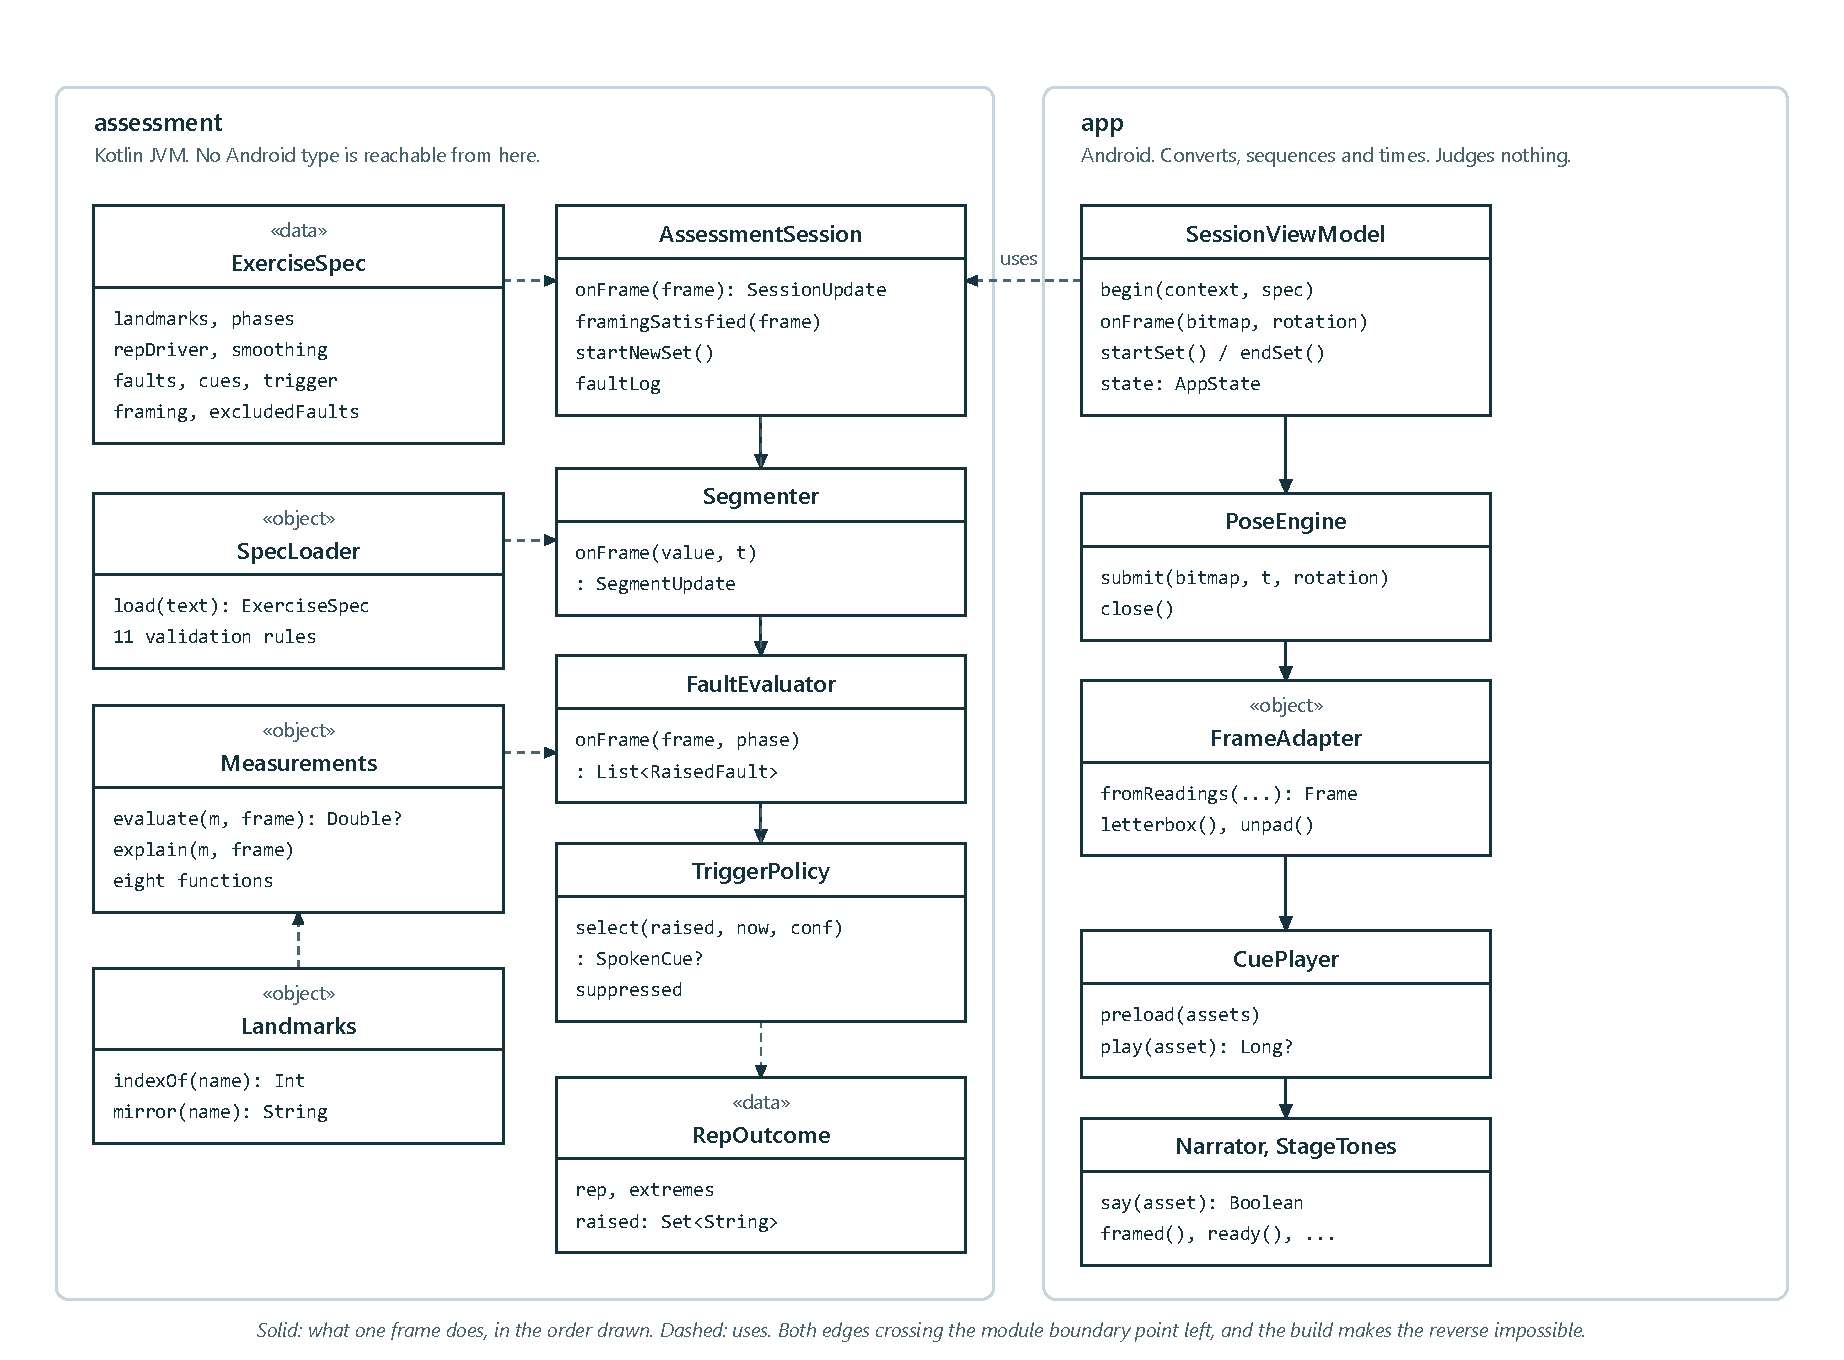
\includegraphics[width=\textwidth]{fig-7-1-classes.pdf}
\caption[The types in the two modules, and the single dependency between them]{The two modules, with every dependency between them pointing in one direction. Nothing on the left can name a type on the right.}
\label{fig:7.1}
\end{figure}

The left column is the assessment module, which is plain Kotlin. The right column is the Android client. There is one edge between them and it points leftward, from the client to the library.

\textbf{The specification, as loaded.}

{\small
\setlength{\LTpre}{6pt}\setlength{\LTpost}{8pt}
\begin{longtable}{>{\raggedright\arraybackslash}p{\dimexpr 0.206\textwidth-2\tabcolsep\relax}>{\raggedright\arraybackslash}p{\dimexpr 0.794\textwidth-2\tabcolsep\relax}}
\caption{The specification as loaded}\\
\toprule
Type & Role \\
\midrule
\endfirsthead
\toprule
Type & Role \\
\midrule
\endhead
\bottomrule
\endfoot
\bottomrule
\endlastfoot
\texttt{Exercise\allowbreak{}Spec} & The parsed file. Landmarks, framing, driver, phases, faults, cues, trigger, exclusions \\
\texttt{Spec\allowbreak{}Loader} & Parses and validates. Eleven rules, each failing with the rule named \\
\texttt{Landmarks} & Name to index, and the mirror of a name. The only type that knows the engine's layout \\
\texttt{Measurements} & The eight measurement functions, and the normalisers \\
\end{longtable}
}

\textbf{The live assessment.}

{\small
\setlength{\LTpre}{6pt}\setlength{\LTpost}{8pt}
\begin{longtable}{>{\raggedright\arraybackslash}p{\dimexpr 0.285\textwidth-2\tabcolsep\relax}>{\raggedright\arraybackslash}p{\dimexpr 0.715\textwidth-2\tabcolsep\relax}}
\caption{The live assessment}\\
\toprule
Type & Role \\
\midrule
\endfirsthead
\toprule
Type & Role \\
\midrule
\endhead
\bottomrule
\endfoot
\bottomrule
\endlastfoot
\texttt{Assessment\allowbreak{}Session} & The one object the client talks to. Takes a frame, returns a \texttt{Session\allowbreak{}Update} \\
\texttt{Segmenter} & Driver, smoothing, hysteresis, phases, counts and hold duration \\
\texttt{Fault\allowbreak{}Evaluator} & Continuous faults: the streak over the declared phases \\
\texttt{Trigger\allowbreak{}Policy} & Which raised fault, if any, becomes a cue \\
\texttt{Rep\allowbreak{}Outcome} & What one repetition came to, emitted at every closing boundary \\
\end{longtable}
}

\textbf{The client.}

{\small
\setlength{\LTpre}{6pt}\setlength{\LTpost}{8pt}
\begin{longtable}{>{\raggedright\arraybackslash}p{\dimexpr 0.480\textwidth-2\tabcolsep\relax}>{\raggedright\arraybackslash}p{\dimexpr 0.520\textwidth-2\tabcolsep\relax}}
\caption{The client}\\
\toprule
Type & Role \\
\midrule
\endfirsthead
\toprule
Type & Role \\
\midrule
\endhead
\bottomrule
\endfoot
\bottomrule
\endlastfoot
\texttt{Session\allowbreak{}View\allowbreak{}Model} & Sequences a session and holds the state the interface renders \\
\texttt{Pose\allowbreak{}Engine} & Loads the model, runs inference, drops a frame that arrives while busy \\
\texttt{Frame\allowbreak{}Adapter} & Letterbox and un-pad, presence floor, tensor to named landmarks \\
\texttt{Cue\allowbreak{}Player}, \texttt{Narrator}, \texttt{Stage\allowbreak{}Tones} & Audio: the fault cues, the spoken stages, the non-verbal markers \\
\end{longtable}
}

Two aspects of the arrangement carry most of its value.

\textbf{\texttt{Assessment\allowbreak{}Session} is the only entry point.} The client does not reach into the segmenter or the evaluator. It calls \texttt{on\allowbreak{}Frame} and receives a phase, a count, the raised faults, and at most one cue. This is what makes the assessment layer replaceable in one place, and it is what the offline replay harness substitutes for.

\textbf{\texttt{Landmarks} is the only type that knows the engine's output layout.} The specifications name landmarks as strings and every measurement resolves them through this one table. Changing the pose engine changed this file and the adapter, and reached no specification and no rule.

\section{Activity Flow}
\label{sec:7.2}

\begin{figure}[htbp]
\centering
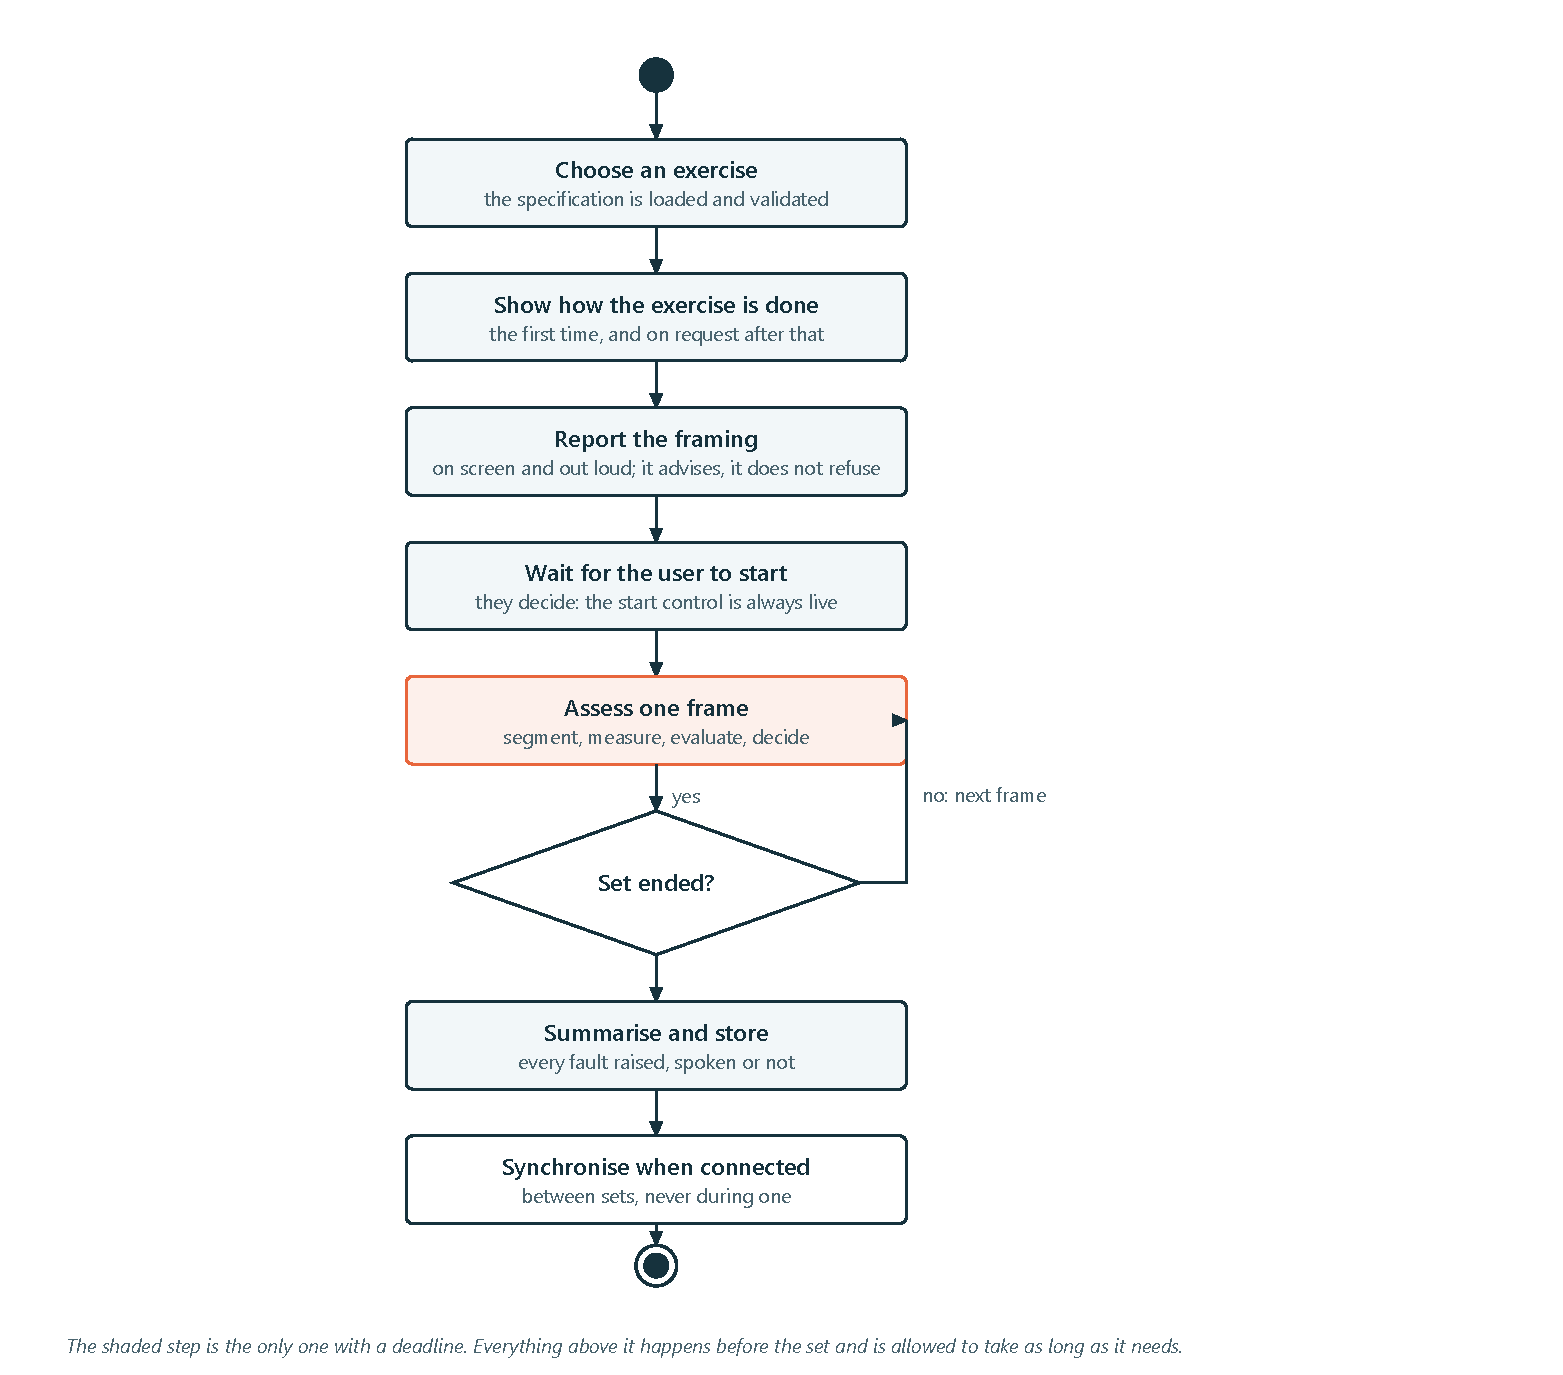
\includegraphics[width=\textwidth]{fig-7-2-session-activity.pdf}
\caption[A session from launch to a written record]{One session. Nothing before the set can send the trainee backwards; the only loop is the frame loop.}
\label{fig:7.2}
\end{figure}

The flow has no gate in it. Before the set the system does two things and blocks on neither: it shows how the exercise is performed, and it reports the framing conditions in the specification, which are the required landmarks visible above the floor and the body occupying a usable part of the frame. When a condition fails the system names the correction needed on screen and goes on naming it. Starting remains one tap throughout. Nothing is spoken before the set except the line confirming it has started: the correction is the same sentence the guide already shows, and a product that reads its own screen aloud while the trainee is standing at it has misread who is where.

An earlier design refused to start until the framing passed. What defeats it is the physical loop: the trainee presses start at the phone and then walks into position, so the framing a pre-set gate measures is the framing of somebody standing beside the camera. The gate was close to free of information and it cost the product the posture of deciding whether a person may train. What the condition genuinely bounds is what the assessment can see, and that is handled where it bites: an unmeasurable landmark makes the faults that need it unmeasured for those frames, which the record states, and the set summary reports what was and was not seen.

Once the set starts it runs without interaction. The trainee's hands are occupied and the screen faces away from them, so everything between the start and the end of a set is audio, which NFR-U1 and NFR-U2 require.

At the end the system stops the pipeline, writes the record, and shows the summary. The summary is the first thing in the whole flow that assumes the trainee is looking at the screen.

\section{Sequence: One Frame to One Cue}
\label{sec:7.3}

\begin{figure}[htbp]
\centering
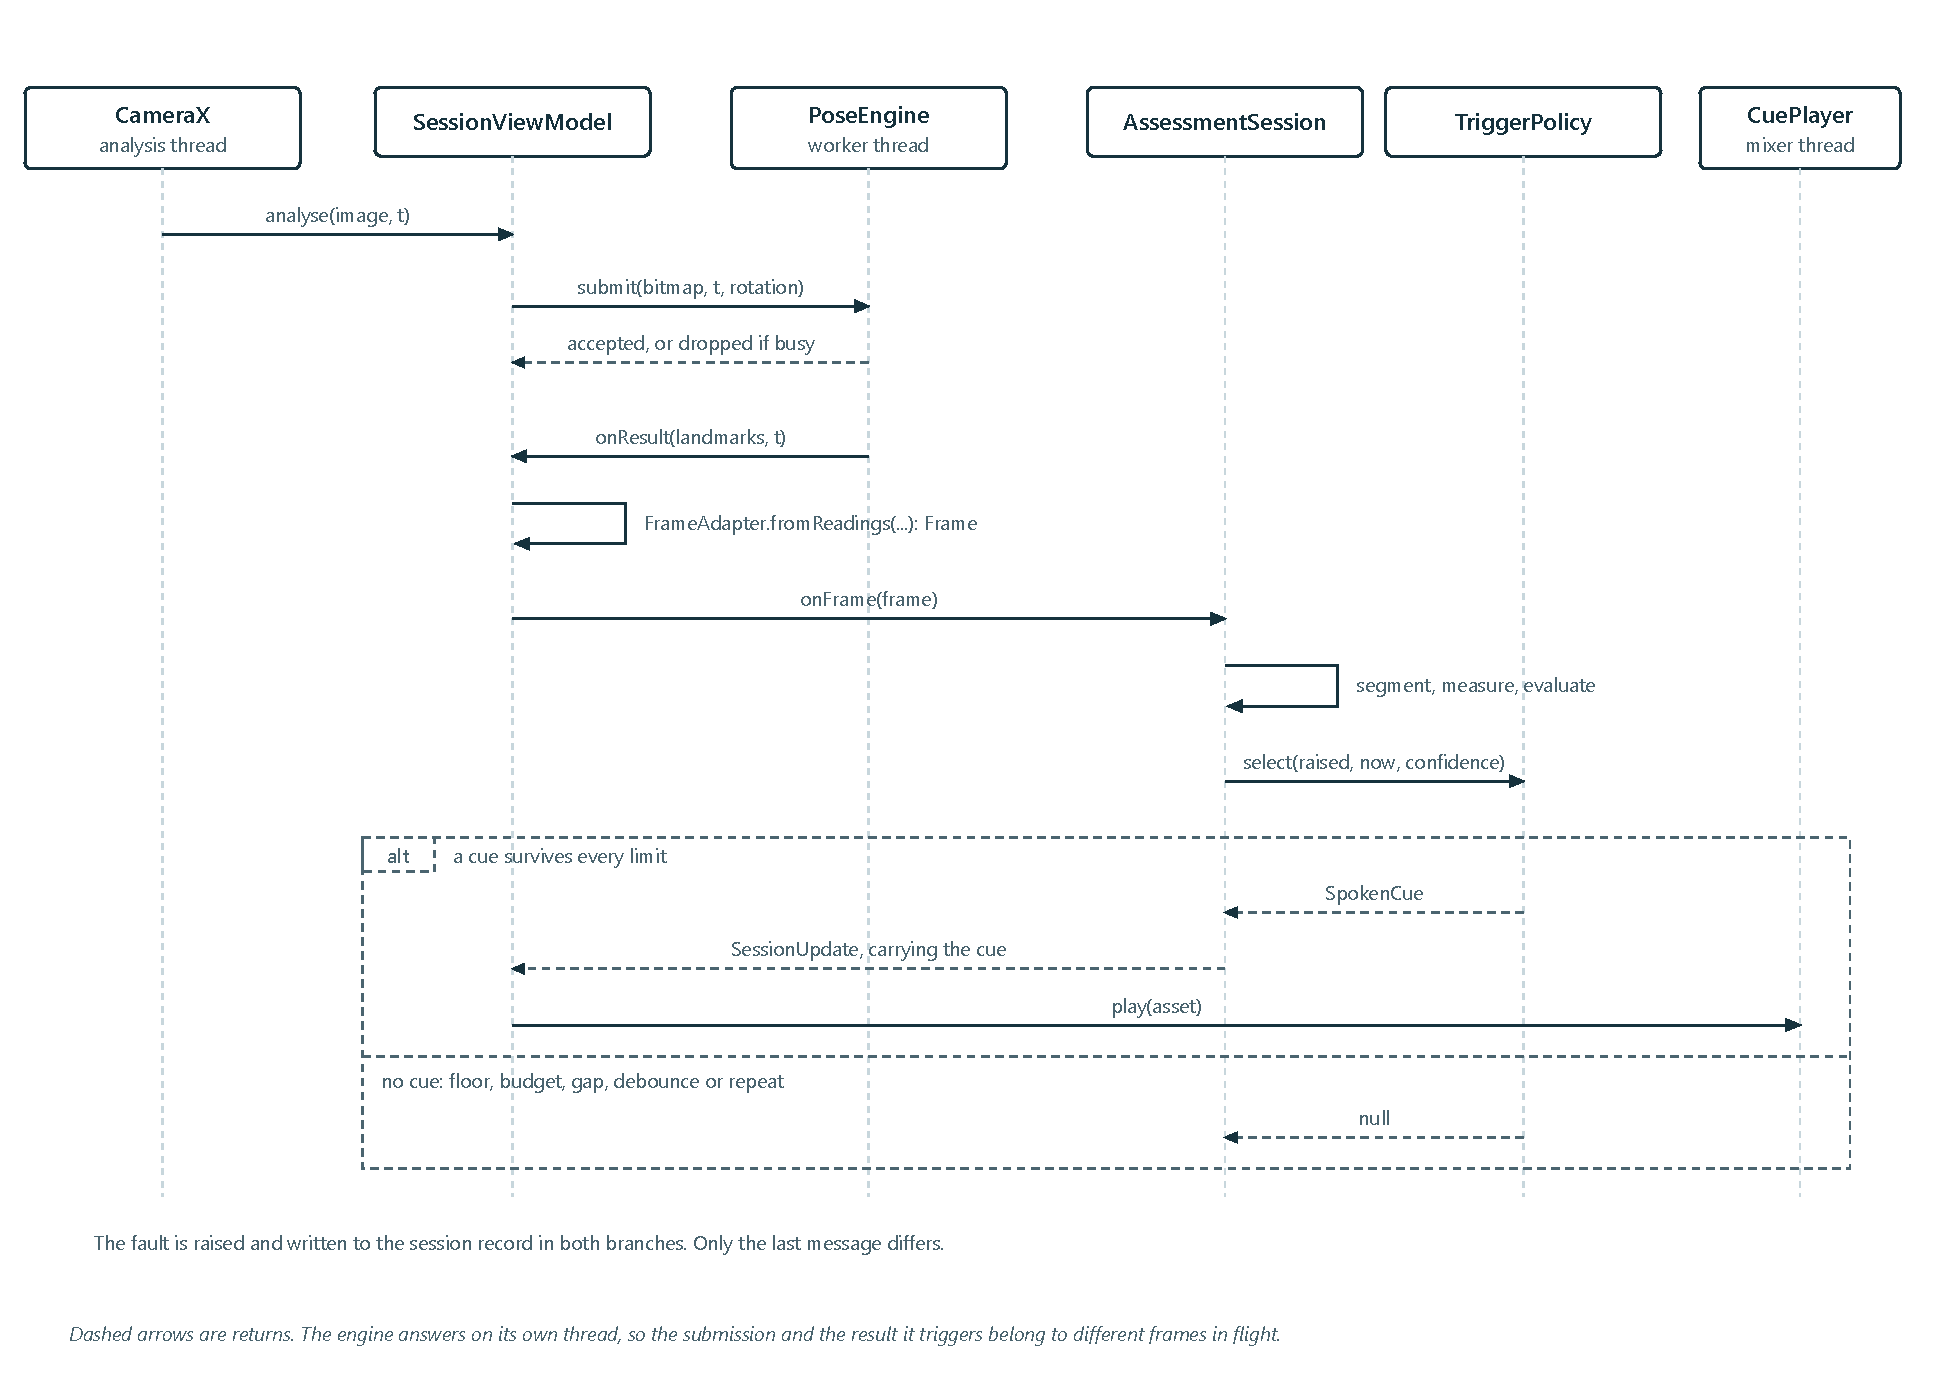
\includegraphics[width=\textwidth]{fig-7-3-frame-to-cue.pdf}
\caption[The call sequence for a single frame, including the paths that end in silence]{One frame. Most frames take one of the early exits.}
\label{fig:7.3}
\end{figure}

The sequence is worth reading for its exits rather than its happy path. A frame can stop at the busy check, at the pose result, at the visibility floor, at the phase scope, at the confirmation streak, at the confidence floor, or at the rate limit. Each is a different reason, and the common case is that a frame stops at one of them.

Three points in the sequence decide the latency the trainee experiences.

\textbf{The timestamp is taken at capture, not at arrival.} Everything downstream measures from when the camera saw the movement rather than from when the application got round to it, so a queueing delay cannot hide inside the figure.

\textbf{The cue is a clip already in memory.} \texttt{Cue\allowbreak{}Player.\allowbreak{}preload} loads every asset the specification names when the session begins, so the path from a confirmed fault to the first audible sample is a map lookup and a play call. There is no file read and no synthesis in it, which is what makes the allocation in 3.4.1 met by construction.

\textbf{The record of what was spoken is taken from the audio layer}, not from the decision to speak. The two differ whenever the policy suppresses, and keeping them separate is what lets a set report six faults raised and two cues spoken without the two numbers contradicting each other.

\section{State Machines}
\label{sec:7.4}

\begin{figure}[htbp]
\centering
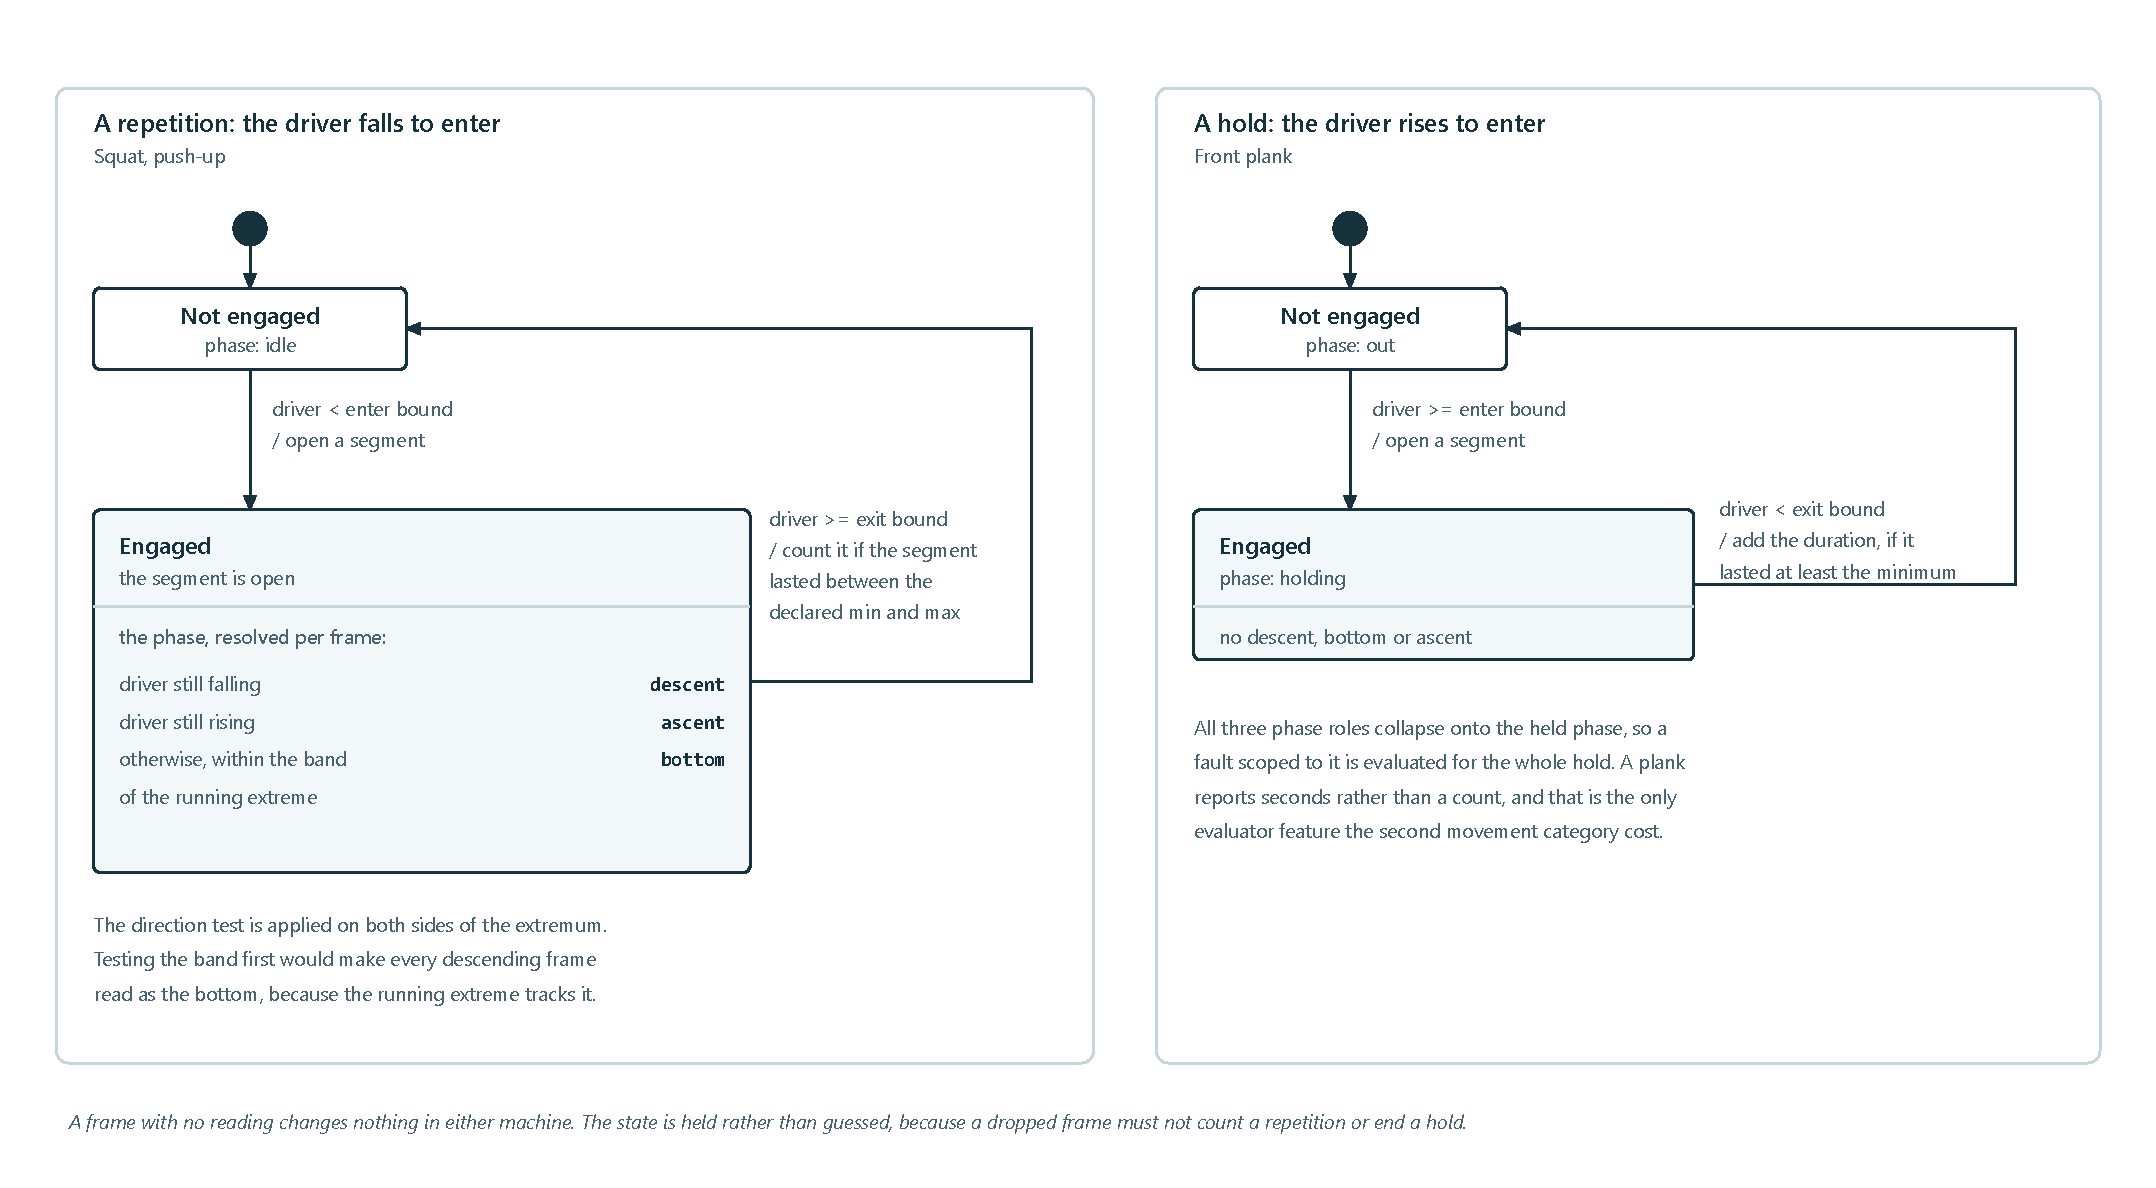
\includegraphics[width=\textwidth]{fig-7-4-segmenters.pdf}
\caption[The counting segmenter and the hold segmenter, side by side]{The same machine twice. Only the entry comparison and what is reported at the end differ.}
\label{fig:7.4}
\end{figure}

The segmenter is one state machine with two configurations.

\textbf{Counting.} Idle until the driver falls below the entry bound; engaged until it rises past the completion bound. On completion, the elapsed time is checked against the declared bounds and the count advances if it passes. Within the engaged state the phase is resolved from the direction of travel: falling is the descent, rising is the ascent, and a driver that has stopped moving within a band of its own extreme is the bottom.

\textbf{Holding.} The same machine with the entry comparison reversed. Entered when the driver rises past its bound, left when it falls back under the other, and the time accumulated rather than counted.

Three details in the implementation are worth naming.

\textbf{Stillness is tested against the measurement's own noise.} The bottom phase is where the driver has stopped moving, which requires a threshold for what counts as movement. That threshold has to sit above the frame-to-frame noise of the pose estimate or the phase is never entered at all. It is a property of the engine rather than of the movement, and 4.2.5 records what happened when it was carried across an engine change unchanged.

\textbf{An unmeasurable driver does not reset the machine.} At the bottom of a squat the ankle can leave the frame, and the driver stops resolving. The segmenter holds its state and reports the phase it was in, rather than treating a missing measurement as a return to idle. This is why the per repetition evaluation mode samples every engaged frame instead of the frames at the driver's extreme.

\textbf{The duration bounds are applied at the close, not during.} A segment is only rejected once its length is known, so a trainee pausing mid-repetition is not cut off partway through; the repetition simply does not count when it ends.

\subsection{The declared phase conditions are not parsed}
\label{sec:7.4.1}

The specification describes each phase in prose: the bottom is \textit{``driver at local minimum, within 10 degrees of it''}. The evaluator does not parse that sentence. The band is a constant in the segmenter, and the phase names in the file are matched to roles by position.

This is a real gap between what the format appears to declare and what the evaluator reads, and it is recorded rather than closed. The effect is bounded: a new exercise in either supported category gets the same phase behaviour as the existing ones whatever its prose says, and an exercise needing different phase semantics needs an evaluator change and not only a file.

It is stated here because a reviewer reading the specification would otherwise reasonably believe the sentence was executable.

\section{Data Model}
\label{sec:7.5}

One record per set, written locally when the set ends.

{\small
\setlength{\LTpre}{6pt}\setlength{\LTpost}{8pt}
\begin{longtable}{>{\raggedright\arraybackslash}p{\dimexpr 0.413\textwidth-2\tabcolsep\relax}>{\raggedright\arraybackslash}p{\dimexpr 0.587\textwidth-2\tabcolsep\relax}}
\caption{The set record written when a set ends}\\
\toprule
Field & Contents \\
\midrule
\endfirsthead
\toprule
Field & Contents \\
\midrule
\endhead
\bottomrule
\endfoot
\bottomrule
\endlastfoot
\texttt{exercise}, \texttt{spec\_\allowbreak{}id}, \texttt{spec\_\allowbreak{}version} & Which exercise, and the version of the file in force \\
\texttt{started\_\allowbreak{}at}, \texttt{ended\_\allowbreak{}at}, \texttt{duration\_\allowbreak{}s} & When the set ran, and how long it took \\
\texttt{reps} or \texttt{hold\_\allowbreak{}s} & The result, by the exercise's declared scoring mode \\
\texttt{reps\_\allowbreak{}with\_\allowbreak{}fault} & How many repetitions carried any fault \\
\texttt{faults}, \texttt{cues} & Every fault raised, and every cue actually spoken, each with its timing \\
\texttt{reps\_\allowbreak{}detail} & One row per repetition: its number, the measured value behind each per-repetition fault, and what was raised \\
\texttt{cues\_\allowbreak{}spoken} & How many the trainee actually heard \\
\texttt{suppressed} & Why a raised fault did not become a cue, counted by reason \\
\texttt{measured} & Per fault, the range of values seen and how many frames were measurable \\
\texttt{pose\_\allowbreak{}rate}, \texttt{fps} & The coverage behind the whole record \\
\end{longtable}
}

\textbf{\texttt{spec\_\allowbreak{}version} is what makes an old record readable.} A fault code means what the specification of that version said it meant. A record without its version becomes uninterpretable the first time a threshold moves, and thresholds in this project have moved.

\textbf{\texttt{reps\_\allowbreak{}detail} stores the value for every repetition, including the ones that passed.} A count of faults answers how many and not which, and it cannot distinguish a set of repetitions that were comfortably correct from a set that passed by a hair. The per-repetition value is what makes a later reader able to tell those apart, and it is what the evaluation in 9.4 is computed from.

\textbf{\texttt{pose\_\allowbreak{}rate} is kept because it qualifies everything else.} A set in which the engine lost the body for a quarter of its frames has a repetition count and a fault count that mean less than the same numbers from a set with full coverage. Storing it means the qualification travels with the record instead of being lost. \texttt{suppressed} and \texttt{measured} are there for the same reason from the other direction: a quiet set and a set that detected nothing look identical without them.

Records are held in application-private storage. Nothing else about a session is written: no frame, no still image and no landmark sequence. That is what NFR-S1 asserts, and a reader can check it by looking for a write path and finding none.

\chapter{UI/UX Design}
\label{chap:8}

\section{Design Principles}
\label{sec:8.1}

The interaction model here is unusual, and the unusual part drives every decision in this chapter: \textbf{during the activity the product is designed for, the trainee can neither look at the screen nor touch it.} They are mid-squat, two to four metres away, facing a direction the designer does not control.

Five principles follow.

\textbf{P1. Audio is the primary output during a set; the screen is secondary.} Anything that must reach the trainee mid-repetition is spoken. The display carries only what survives a one-second glance from three metres: the repetition count, and whether the system is tracking.

\textbf{P2. All configuration happens before the set and none during it.} Exercise selection, setting up and settings are pre-set activities. Once a set starts the only interaction available is ending it, which is NFR-U1.

\textbf{P3. Everything the trainee has to get right is said before the set, and nothing is withheld until they get it right.} Before the first set of an exercise the product shows the position it measures against, where to put the phone, and what each cue will ask for. During set-up it reports the framing and keeps reporting it. It does not refuse to start: 7.2 gives the reason, which is that the trainee presses start at the phone and then walks into position, so a gate there grades the wrong moment.

\textbf{P4. The posture is the device standing unaided, folded to ninety degrees.} The target handset does this without a tripod, which is why none is required. The camera and the main display face the trainee together, and \textbf{only the upper half of the display is visible in that posture}, so every screen places what the trainee must see in the upper half. The constraint is held in the layouts rather than drawn on them.

\textbf{P5. Nothing is shown that was not measured.} Where the interface shows a number, it shows what that number is. A repetition count is a count and a fault count is a count. No accuracy percentage, confidence score or overall form score appears anywhere, because no such figure could be defended.

\textbf{Physical constraints are design inputs rather than afterthoughts.} The viewing distance is two to four metres, so type must be large. Hands may be sweaty and the trainee out of breath, so pre-set targets must be large and few. Ambient lighting is uncontrolled, so contrast must be high. The room may be noisy, which is why headphones are assumed.

\section{Screen Inventory}
\label{sec:8.2}

{\small
\setlength{\LTpre}{6pt}\setlength{\LTpost}{8pt}
\begin{longtable}{>{\raggedright\arraybackslash}p{\dimexpr 0.090\textwidth-2\tabcolsep\relax}>{\raggedright\arraybackslash}p{\dimexpr 0.244\textwidth-2\tabcolsep\relax}>{\raggedright\arraybackslash}p{\dimexpr 0.666\textwidth-2\tabcolsep\relax}}
\caption{The nine screens, and what each one is for}\\
\toprule
\# & Screen & Purpose \\
\midrule
\endfirsthead
\toprule
\# & Screen & Purpose \\
\midrule
\endhead
\bottomrule
\endfoot
\bottomrule
\endlastfoot
S1 & Home & Start a set, or open history \\
S2 & Exercise selection & Choose from the exercises whose specifications are loaded \\
S3 & Set-up & Live preview with the specific correction needed, and the guide to the exercise \\
S4 & Live session & Repetition count, tracking state, end control \\
S5 & Set summary & Repetitions, faults and counts, immediately after the set \\
S6 & Session history & Reverse chronological list \\
S7 & Session detail & Per-set breakdown \\
S8 & Fault detail & Plain-language description, the cue spoken, what to do differently next time, and the source of the definition \\
S9 & Settings & A sound check before a set \\
\end{longtable}
}

Three of these exist because of commitments made elsewhere in the report.

\textbf{S3 exists because of FR-02 and FR-28.} What it shows is the specific correction rather than a generic failure: move further back, turn side on. A screen that said only ``framing not usable'' would leave the trainee to guess. It also carries the guide, which opens over it on the first set of an exercise and is reachable from it afterwards. The guide is the one place the product explains the movement instead of judging it. The diagram on it draws the line the faults are measured against, so the standard is visible before it is applied.

\textbf{S8 exists because of O5.} Every fault the system can raise traces to a published criterion, and S8 is where that reaches the trainee. It shows the plain-language description, the cue that was spoken, what to do differently next time, and where the definition came from. A system that asserts a fault without being able to say why it is a fault has not earned the correction, and one that says what is wrong without saying what to do about it has stopped half way.

\textbf{The source is shown in a sentence, not as a citation.} The specification carries both: the reference, with authors, journal and the quoted criterion, and the same claim written for somebody holding a phone. The screen shows the second. The first belongs in this report. An earlier build printed the opening of it on screen and the line ended mid-clause, which is what a citation looks like in a place it does not fit.

\textbf{S9 exists for one reason the trainee can act on.} The product corrects out loud, and their headphones, their volume and their silent switch are three things it depends on entirely and cannot see. Finding out mid-set that the phone was muted costs them the set, so the screen is a sound check and little else.

Everything else that screen used to carry, including the loaded specification versions, was written for a reviewer rather than for a trainee and has been removed. The provenance of a fault reaches the user through S8, where it is attached to a correction they actually heard, which is the only place it means anything to them.

\section{Screen Flow}
\label{sec:8.3}

\begin{figure}[htbp]
\centering
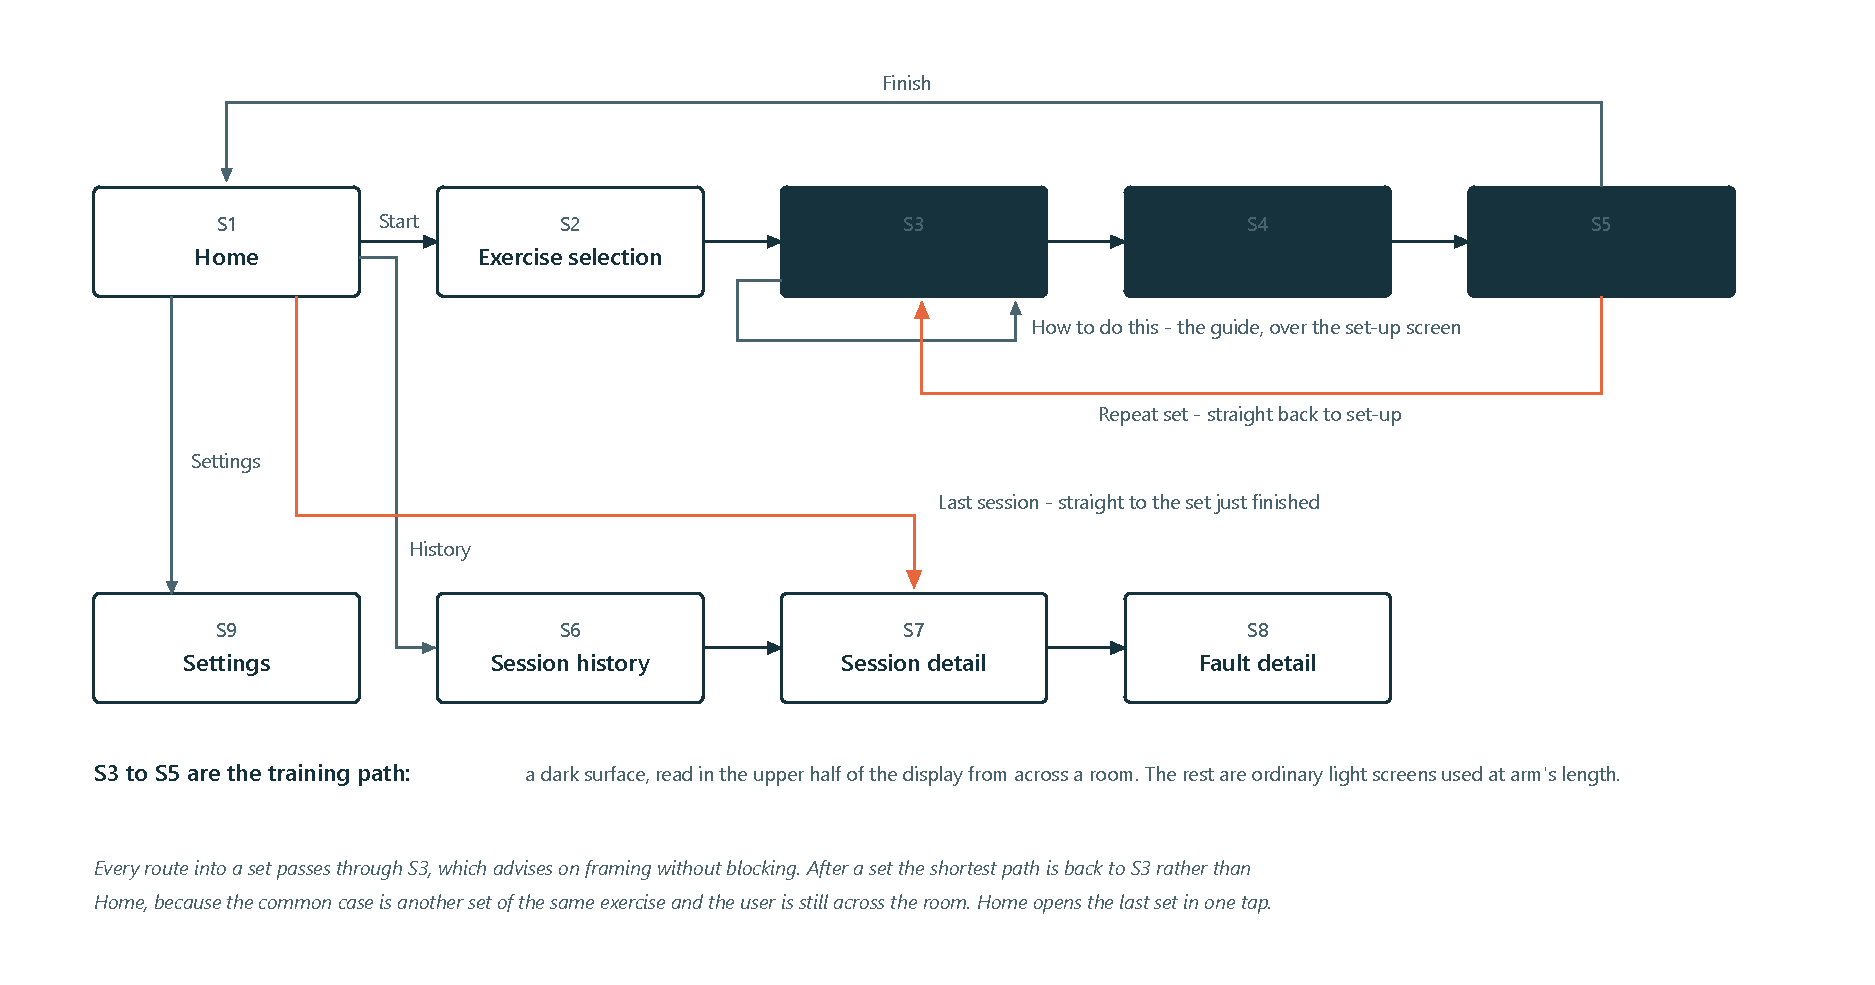
\includegraphics[width=\textwidth]{fig-8-1-screen-flow.pdf}
\caption[How the nine screens connect, and the two paths through them]{The training path across the top and the history path below. The two accented edges are the shortcuts: back to set-up after a set, and straight from Home into the set just finished.}
\label{fig:8.1}
\end{figure}

Three properties of the flow are deliberate.

\textbf{Set-up is on the path and cannot be bypassed, but it cannot block either.} Every route into a set passes through it, so the framing is always reported and the guide is always one tap away; neither is a condition of starting.

\textbf{After a set, the shortest path is back to set-up rather than to Home.} The common case after a set is another set of the same exercise, and the trainee is still across the room. Routing them through Home would make the most frequent action the longest one. The guide does not reopen on a repeat: they have just done the exercise.

\textbf{Home opens the last set directly, without going through the list.} The card on Home already names that set, and somebody who has just finished training and picked the phone back up wants that one set far more often than they want every set they have ever done. Making them pass through S6 to reach a record S1 was already showing them is the list existing for its own sake. S6 remains the only route to everything else, and S7 knows which way it was entered so that back goes where the trainee came from.

\section{Visual Language}
\label{sec:8.4}

The design file is built on \textbf{bound design tokens rather than literal values}: fourteen colour variables, eight spacing steps, four radii and a ten-step type ramp, each bound in the file rather than typed into a shape. The colour meanings asserted here are therefore enforced by the file instead of merely described by it.

\textbf{Colour carries exactly one meaning, and it is state.} A fault is warm, a pass is cool, and everything structural is neutral. Nothing is coloured for decoration, because a palette that colours both decoration and state cannot be read at a glance from three metres, which is the only reading condition that matters during a set.

\textbf{Type is sized for distance rather than for density.} The repetition count is the largest element on the live screen by a wide margin, because it is the one number the trainee may glance at mid-set. Everything else on that screen is deliberately subordinate.

\section{Prototype}
\label{sec:8.5}

A navigable prototype covering S1 through S9, built in Figma across three pages: the brand, the screens at 412 by 990, and the screen flow. That is the common Android reference frame, not a measurement of the target handset. The handset's main display is 1080 by 2640 physical pixels, which is 384 by 939 device-independent pixels at the display density set on the test device, so the prototype is drawn a little larger than the screen it is for. Ten artboards cover the nine screens, because S3 has two states worth drawing: the set-up screen and the guide that opens over it. The guide's artboard is taller than a handset screen, which is deliberate: it scrolls, and drawing it at 990 would have shown a button cut in half rather than a sheet.

\textbf{The guide shows a photograph, not a drawing.} The first version drew the line each rule measures against, which is a useful thing for a diagram to do and not what somebody about to train wants to look at. Every photograph the product ships is licensed for it, and \texttt{docs/\allowbreak{}assets/\allowbreak{}ui/\allowbreak{}CREDITS.\allowbreak{}md} records the source, the author and the licence of each. The squat shown here is by Matt Moloney on StockSnap, released under CC0.

\begin{figure}[htbp]
\centering
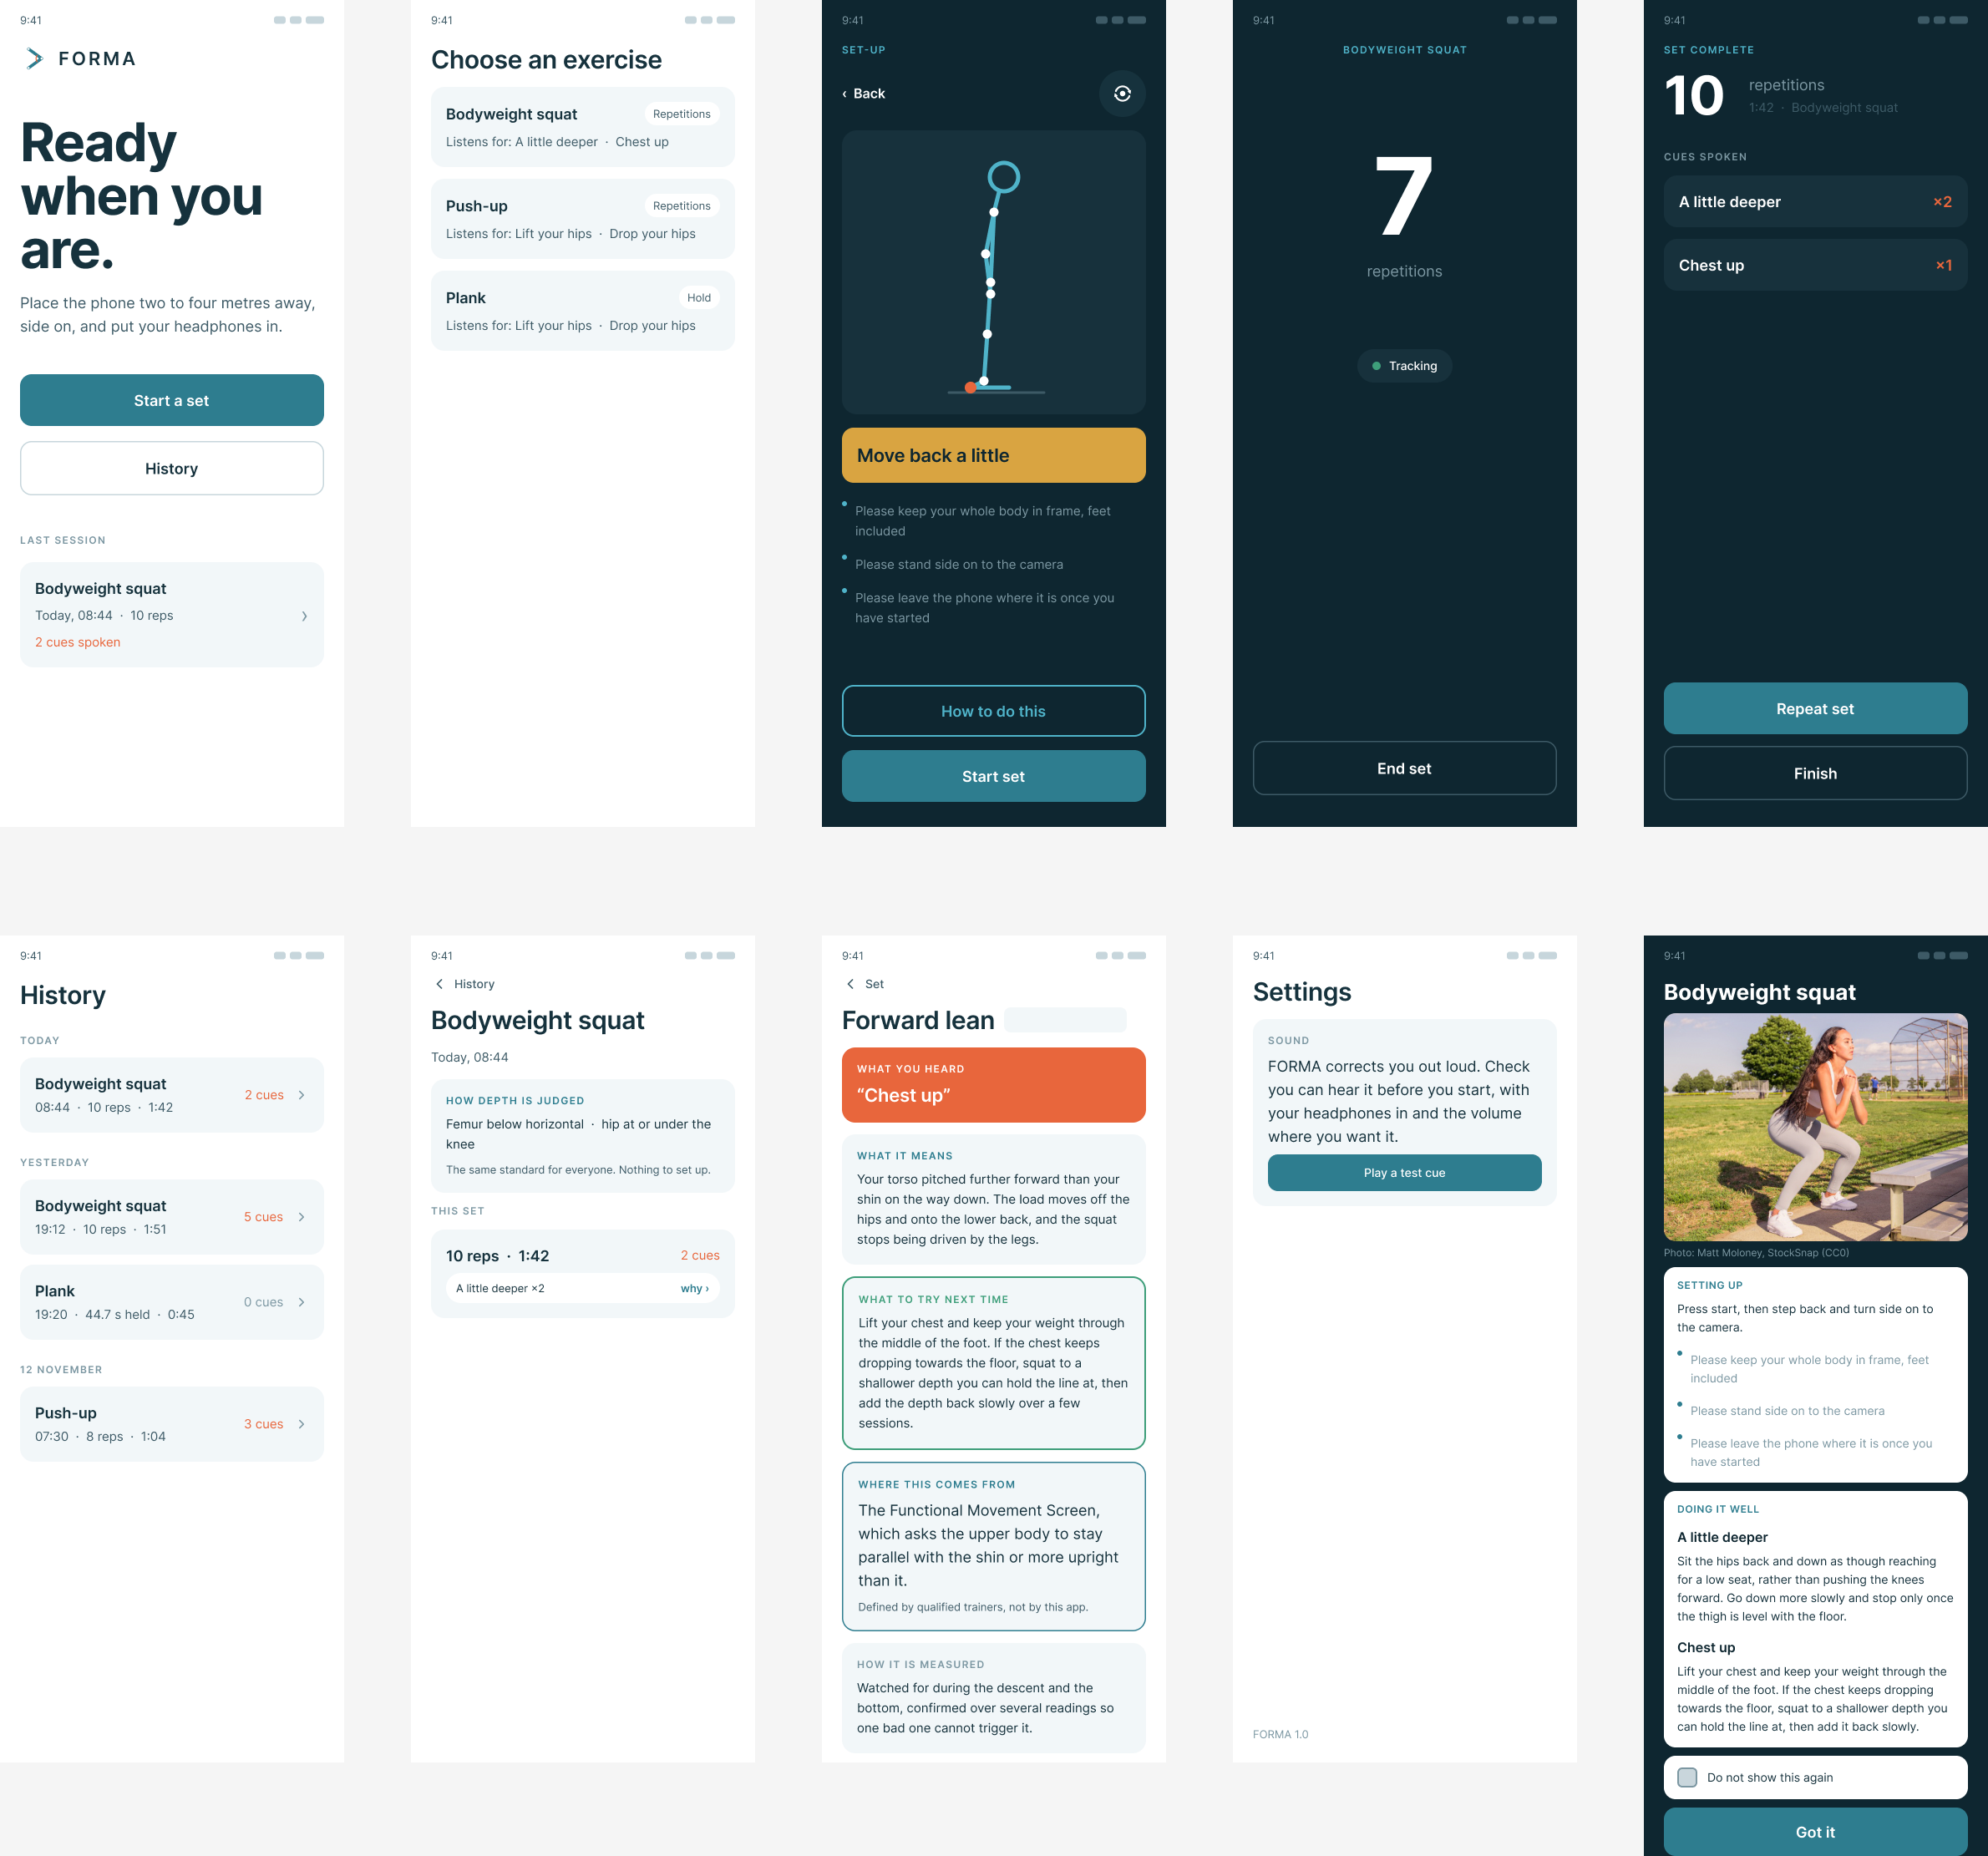
\includegraphics[width=\textwidth]{forma-screens.png}
\caption[The nine screens at 412 by 990, with the guide that opens over S3]{The nine screens, with the guide that opens over S3. The training path is laid out for the upper half of the display, which is what the folded posture leaves visible.}
\label{fig:8.2}
\end{figure}

\textbf{What the prototype demonstrates.} The flows, the information hierarchy, and the screen states, including the two that are easiest to leave undesigned: framing that needs correcting, and a fault that has no authored cue. Both are states the system genuinely reaches, and both have a designed appearance rather than an undefined one.

\textbf{What the prototype cannot establish, and what was checked on the device instead.} Legibility at three metres and usability while out of breath are properties of the handset in the real posture, not of a design file. Both were checked on the target device. The repetition count and the tracking state were readable at three metres in a glance, and the controls were operable immediately after a set taken to near failure. This is one person on one device, so it is an observation and not a usability study; what it rules out is the failure that would have mattered most, which is type sized for a desk and controls sized for a steady hand.

This is the bar the supervisor set for this phase: a UI/UX demonstration is sufficient evidence of the product surface, and it does not need a shipped application behind it.

\chapter{Proof of Concept and Results}
\label{chap:9}

\section{Scope of the Proof of Concept}
\label{sec:9.1}

This phase builds the part of the product that decides whether the rest is worth building: the path from a camera frame to a spoken correction, running on a handset, for three exercises.

\textbf{What was built.} The assessment library and its specification format, a mobile client carrying camera, model, interface and audio, a separate benchmark application for measuring the engine, and an offline replay harness that scores recorded video through exactly the shipped logic. Three exercise specifications, six faults, and a cue for each.

\textbf{What was deliberately left out.} Everything in 1.4.2's second phase: no language is generated anywhere in this system. There is no programme generation, no nutrition, and no conversational layer. The server is specified and its contract is fixed by FR-16 to FR-18; it is not built in this phase, and 11.3 records that against the objective it serves. \textbf{FR-11, creating an account and signing in, goes with it}, since there is nothing to sign in to.

\textbf{FR-15, deleting a session, is also not built, and it has no such excuse.} A record is one file in the application's own storage and removing it needs no server. It is named here rather than left for a reader to notice.

The bar for this phase was set by the supervisor and is narrower than a shipped product: a proof of concept, a demonstration and a prototype. The measurements below are reported against that bar.

\section{Implementation}
\label{sec:9.2}

{\small
\setlength{\LTpre}{6pt}\setlength{\LTpost}{8pt}
\begin{longtable}{>{\raggedright\arraybackslash}p{\dimexpr 0.524\textwidth-2\tabcolsep\relax}>{\raggedright\arraybackslash}p{\dimexpr 0.201\textwidth-2\tabcolsep\relax}>{\raggedright\arraybackslash}p{\dimexpr 0.275\textwidth-2\tabcolsep\relax}}
\caption{What was built, in files and lines}\\
\toprule
 & Files & Lines \\
\midrule
\endfirsthead
\toprule
 & Files & Lines \\
\midrule
\endhead
\bottomrule
\endfoot
\bottomrule
\endlastfoot
\texttt{assessment}, main & 9 & 2,057 \\
\texttt{assessment}, tests & 12 & 2,201 \\
\texttt{app}, main & 11 & 3,086 \\
\texttt{app}, tests & 1 & 129 \\
Benchmark application & 4 & 1,483 \\
Replay harness & 1 & 680 \\
Specifications & 3 & 538 \\
\end{longtable}
}

Two ratios in that table are the ones worth reading.

\textbf{The assessment module has more test code than production code}, 2,201 lines against 2,057. That is a consequence of the module having no Android dependency: because a recorded landmark sequence can be replayed through it as an ordinary unit test, testing it is cheap enough to be worth doing thoroughly.

\textbf{The specifications are 538 lines for three exercises}, and most of that is provenance rather than rules. Each fault carries the source its definition came from and the derivation of its threshold, in the file, because the format will not accept a fault without them.

The client is Kotlin on Android: CameraX for capture, TFLite for pose, Jetpack Compose for the interface. A set is written as one JSON file in the application's own storage and read back from there, so there is no database and no schema migration to carry; 7.5 lists what a record holds. The assessment library depends on nothing but a JSON parser.

\section{Measurement Method}
\label{sec:9.3}

Three instruments, each measuring something the others cannot.

\textbf{The benchmark application} drives the pose engine and nothing else. It shares no source with the client, so a figure attributed to it describes a fixed artefact rather than a build that has since changed. It measures frame rate and per-frame latency, and it cannot measure anything downstream of the engine because none of it is present. Appendix A describes it and names every run.

\textbf{The test suite} runs the assessment layer against synthetic landmark sequences on a desktop JVM, with no device in the loop. It establishes that the evaluator does what the specification says, which is a different question from whether the specification describes the movement correctly.

\textbf{The replay harness} closes the gap between the two. It runs a recorded video through the shipped model file with the same letterbox, the same presence floor, the same visibility floor, the same median smoothing, the same hysteresis and the same rules as the handset, and writes a per-frame record and a per-repetition verdict. Because the recordings are scripted, the correct answer for each is known before the system is run against it.

\textbf{One caveat applies to every replay figure and is stated once here.} The harness runs TFLite on the desktop CPU, while the handset runs the GPU delegate. Verdicts are unaffected, because the model file and the arithmetic are identical; timings from the harness are not comparable to the device and none is quoted.

\subsection{The recorded dataset}
\label{sec:9.3.1}

Ten sets, filmed in one session in a single camera position, left side to the camera at hip height.

{\footnotesize
\setlength{\LTpre}{6pt}\setlength{\LTpost}{8pt}
\begin{longtable}{>{\raggedright\arraybackslash}p{\dimexpr 0.230\textwidth-2\tabcolsep\relax}>{\raggedright\arraybackslash}p{\dimexpr 0.150\textwidth-2\tabcolsep\relax}>{\raggedright\arraybackslash}p{\dimexpr 0.161\textwidth-2\tabcolsep\relax}>{\raggedright\arraybackslash}p{\dimexpr 0.459\textwidth-2\tabcolsep\relax}}
\caption{The ten recorded sets}\\
\toprule
Set & Exercise & Performed & Scripted condition \\
\midrule
\endfirsthead
\toprule
Set & Exercise & Performed & Scripted condition \\
\midrule
\endhead
\bottomrule
\endfoot
\bottomrule
\endlastfoot
\texttt{SQ-\allowbreak{}CLEAN} & Squat & 10 reps & correct \\
\texttt{SQ-\allowbreak{}SHALLOW} & Squat & 10 reps & stop above parallel \\
\texttt{SQ-\allowbreak{}LEAN} & Squat & 10 reps & pitch the torso forward \\
\texttt{PU-\allowbreak{}CLEAN} & Push-up & 10 reps & correct \\
\texttt{PU-\allowbreak{}SAG} & Push-up & 10 reps & hips dropped \\
\texttt{PU-\allowbreak{}PIKE} & Push-up & 10 reps & hips raised \\
\texttt{PU-\allowbreak{}RANGE} & Push-up & 10 reps & body line held, range of motion varied \\
\texttt{PL-\allowbreak{}CLEAN} & Plank & 44.7 s & correct \\
\texttt{PL-\allowbreak{}SAG} & Plank & 47.6 s & hips dropped \\
\texttt{PL-\allowbreak{}PIKE} & Plank & 47.2 s & hips raised \\
\end{longtable}
}

\texttt{PU-\allowbreak{}RANGE} is a negative control. The body line is held throughout while the range of motion varies, so neither hip fault should fire, and it tests the two push-up rules against a movement that changes in a way they are meant to ignore.

\textbf{The four clean sets are not filler.} They are the only source of a false-positive figure, and a fault detector reported without one has not been evaluated. They were performed with the same care as the fault sets.

The repetition count in the third column is the ground truth, and it was established independently of the system: the driver trace for each set was examined for excursions past the entry bound, which counts repetitions without using the segmenter's own logic. Every set contained ten.

\section{Results}
\label{sec:9.4}

\subsection{Perception}
\label{sec:9.4.1}

{\footnotesize
\setlength{\LTpre}{6pt}\setlength{\LTpost}{8pt}
\begin{longtable}{>{\raggedright\arraybackslash}p{\dimexpr 0.232\textwidth-2\tabcolsep\relax}>{\raggedright\arraybackslash}p{\dimexpr 0.170\textwidth-2\tabcolsep\relax}>{\raggedright\arraybackslash}p{\dimexpr 0.277\textwidth-2\tabcolsep\relax}>{\raggedright\arraybackslash}p{\dimexpr 0.321\textwidth-2\tabcolsep\relax}}
\caption{Perception measured against the requirements it has to meet}\\
\toprule
Configuration & Frames per second & Total latency, 95th percentile & Requirement \\
\midrule
\endfirsthead
\toprule
Configuration & Frames per second & Total latency, 95th percentile & Requirement \\
\midrule
\endhead
\bottomrule
\endfoot
\bottomrule
\endlastfoot
MoveNet Lightning, GPU & 29.57 & 27 ms & NFR-P2 22 fps, NFR-P3 65 ms \\
\end{longtable}
}

From the deciding sweep in 4.2.3, on the target handset. The frame rate is at the camera's own 30 fps ceiling and the latency has 2.4 times the bound in hand. The engine comparison that produced this configuration, and the seven it was chosen over, is in 4.2.

\textbf{Across the ten recorded sets, 9,893 frames were analysed and the engine returned a pose on every one of them.} No frame was lost to detection failure, in any exercise, in any position, including the bottom of a squat and the floor-level positions of the push-up and plank.

\subsubsection*{The frame rate over ten continuous minutes}

NFR-P2 is a floor for a set. NFR-P4 asks whether that floor survives a session, which is a different question: the handset gets hot, and a thermal limit that arrives in the ninth minute does not show up in a sixty-second measurement.

{\small
\setlength{\LTpre}{6pt}\setlength{\LTpost}{8pt}
\begin{longtable}{>{\raggedright\arraybackslash}p{\dimexpr 0.311\textwidth-2\tabcolsep\relax}>{\raggedright\arraybackslash}p{\dimexpr 0.689\textwidth-2\tabcolsep\relax}}
\caption{The frame rate across a ten-minute run, in thirty-second windows}\\
\toprule
Window & Frames per second \\
\midrule
\endfirsthead
\toprule
Window & Frames per second \\
\midrule
\endhead
\bottomrule
\endfoot
\bottomrule
\endlastfoot
0 to 90 s & 29.83, 29.77, 29.70, 29.63 \\
120 to 330 s & 26.33, 25.97, 26.47, 25.23, 26.47, 26.23, 25.80, 26.07 \\
360 to 570 s & 25.00, 25.20, 26.47, 25.20, 25.57, 26.27, 25.63, 25.07 \\
\end{longtable}
}

15,961 frames over 600.1 s on the shipped configuration, MoveNet Lightning on the GPU delegate. \textbf{The lowest of the twenty complete windows is 25.00 fps, against a floor of 22.} The run holds the floor throughout with three frames per second in hand at its worst.

The shape of the decline is the finding rather than the figure. The first two minutes run at the camera's 30 fps ceiling; the rate then settles into a band between 25.0 and 26.5 and stays there for the remaining eight minutes. Median inference time rose from 16 ms in the first minute to 27 ms in the last, battery temperature from 33.8 to 39.0 degrees, and the Android thermal status reached 2. \textbf{The device throttles, the throttling arrives inside the first three minutes, and it then stops getting worse.} The 95th percentile of the whole per-frame path was 40 ms hot, against the 65 ms NFR-P3 allows, so per-frame latency stays inside its own requirement at the temperature the frame rate settles at.

\textbf{The run completed with no crash and no restart}, which is NFR-A5.

\textbf{What this run is not.} The benchmark's framing gate reached its two-minute cap without confirming a subject, and the summary records that in its own note: both knees cleared the visibility floor in 2.0 per cent of frames. Every landmark column in this run is therefore void, and none is quoted.

The frame rate is not, and the run itself shows why. MoveNet Lightning is a single-pose network of fixed cost: it runs the same arithmetic on a 192 by 192 input whether or not anybody is in it. The windows bear that out. The window at 480 s, the only one in the second half with the subject visible in any quantity at 9.4 per cent of frames, reads 25.57 fps, sitting between its neighbours at zero per cent on 25.20 and 26.27. Across the twenty windows the frame rate tracks temperature and shows no relationship to whether a body is in shot.

\textbf{Why the gate did not open is worth recording}, because it is a property of the instrument rather than of the camera placement. The benchmark requires \textbf{both} knees above the floor for a continuous second and a half. The product requires the better of the two, which 6.2 explains: in the sagittal view this system declares, the far knee is occluded by the near leg for much of a repetition. One knee or the other cleared the floor in 43.3 per cent of frames here. The subject was in shot in the posture the product asks for, and the benchmark asked for a different one.

\subsection{Repetition counting}
\label{sec:9.4.2}

{\small
\setlength{\LTpre}{6pt}\setlength{\LTpost}{8pt}
\begin{longtable}{>{\raggedright\arraybackslash}p{\dimexpr 0.575\textwidth-2\tabcolsep\relax}>{\raggedright\arraybackslash}p{\dimexpr 0.223\textwidth-2\tabcolsep\relax}>{\raggedright\arraybackslash}p{\dimexpr 0.202\textwidth-2\tabcolsep\relax}}
\caption{Repetition counting across the seven counting sets}\\
\toprule
Set & Performed & Counted \\
\midrule
\endfirsthead
\toprule
Set & Performed & Counted \\
\midrule
\endhead
\bottomrule
\endfoot
\bottomrule
\endlastfoot
\texttt{SQ-\allowbreak{}CLEAN}, \texttt{SQ-\allowbreak{}SHALLOW}, \texttt{SQ-\allowbreak{}LEAN} & 10 each & 10 each \\
\texttt{PU-\allowbreak{}CLEAN}, \texttt{PU-\allowbreak{}SAG}, \texttt{PU-\allowbreak{}PIKE}, \texttt{PU-\allowbreak{}RANGE} & 10 each & 10 each \\
\end{longtable}
}

\textbf{Seven of seven counting sets exact, for a repetition count error of zero against the NFR-A3 allowance of one.}

The three plank sets report duration rather than a count, at 44.7, 47.6 and 47.2 seconds, each accumulated continuously so that a trainee who ends the set while still in position gets the time they held.

\subsection{Fault detection}
\label{sec:9.4.3}

Each set scripts one condition. A fault is expected in the set that scripts it and must not appear in the sets that do not.

{\footnotesize
\setlength{\LTpre}{6pt}\setlength{\LTpost}{8pt}
\begin{longtable}{>{\raggedright\arraybackslash}p{\dimexpr 0.382\textwidth-2\tabcolsep\relax}>{\raggedright\arraybackslash}p{\dimexpr 0.277\textwidth-2\tabcolsep\relax}>{\raggedright\arraybackslash}p{\dimexpr 0.215\textwidth-2\tabcolsep\relax}>{\raggedright\arraybackslash}p{\dimexpr 0.126\textwidth-2\tabcolsep\relax}}
\caption{Fault detection across the six faults, in the sets that carry them and the sets that do not}\\
\toprule
Fault & Raised in its condition & Raised elsewhere & Precision \\
\midrule
\endfirsthead
\toprule
Fault & Raised in its condition & Raised elsewhere & Precision \\
\midrule
\endhead
\bottomrule
\endfoot
\bottomrule
\endlastfoot
\texttt{SQ\_\allowbreak{}DEPTH\_\allowbreak{}INSUFFICIENT} & 10 of 10 repetitions & 0 & 1.000 \\
\texttt{SQ\_\allowbreak{}FORWARD\_\allowbreak{}LEAN} & 44 frames & 0 & 1.000 \\
\texttt{PU\_\allowbreak{}HIP\_\allowbreak{}SAG} & 273 frames & 0 & 1.000 \\
\texttt{PU\_\allowbreak{}HIP\_\allowbreak{}PIKE} & 199 frames & 9 & 0.957 \\
\texttt{PL\_\allowbreak{}HIP\_\allowbreak{}SAG} & 1,034 frames & 13 & 0.988 \\
\texttt{PL\_\allowbreak{}HIP\_\allowbreak{}PIKE} & 728 frames & 0 & 1.000 \\
\textbf{The five faults judged per frame} & \textbf{2,278 frames} & \textbf{22} & \textbf{0.990} \\
\end{longtable}
}

\textbf{All six faults meet NFR-A1}, which requires a precision of 0.90 or better per fault. The lowest is 0.957.

The aggregate row covers the five faults judged frame by frame. Squat depth is judged once per repetition, so its 10 of 10 is not a quantity that can be added to a frame count. Read the aggregate for what it is: the plank supplies 1,762 of its 2,278 frames, so 0.990 is mostly a statement about the plank.

\textbf{Every scripted condition was detected}, six of six, giving a recall of 1.00 at the level the recordings support. Squat depth, which is judged once per repetition, was detected on 10 of 10 shallow repetitions and on none of the 10 clean ones.

Two results inside that table are worth drawing out.

\textbf{Sag and pike separate completely in both exercises.} In all four of those sets the opposite fault fired on exactly zero frames. These are two deviations of the same body line measured by the same function with opposite signs, and they are the pair most at risk of bleeding into one another. The bands placed against measured neutral in 6.4.3 are what produced the separation.

\textbf{Squat depth separates with room to spare.} Clean repetitions measured +0.012 to +0.038 and shallow ones -0.083 to -0.112, leaving a gap of 0.045 with no observation in it. The threshold at -0.0209 sits inside that gap.

The 22 frames in the false-positive column are two episodes: 13 frames in the clean plank, which is 1 per cent of a 44.7 second hold, and 9 frames in \texttt{PU-\allowbreak{}RANGE}, which is 1 per cent of that set.

\subsection{The feedback path on the device}
\label{sec:9.4.4}

Fourteen sets were performed on the handset with the application running, and the session record timestamps the cue path. Over the twelve cues spoken by the current build:

{\small
\setlength{\LTpre}{6pt}\setlength{\LTpost}{8pt}
\begin{longtable}{>{\raggedright\arraybackslash}p{\dimexpr 0.429\textwidth-2\tabcolsep\relax}>{\raggedright\arraybackslash}p{\dimexpr 0.317\textwidth-2\tabcolsep\relax}>{\raggedright\arraybackslash}p{\dimexpr 0.254\textwidth-2\tabcolsep\relax}}
\caption{The feedback path on the device, measured against the budget in 3.4.1}\\
\toprule
Stage & Measured & Allocation in 3.4.1 \\
\midrule
\endfirsthead
\toprule
Stage & Measured & Allocation in 3.4.1 \\
\midrule
\endhead
\bottomrule
\endfoot
\bottomrule
\endlastfoot
Trigger policy, confirmation to selection & 0 ms & 5 ms \\
Selection to audio dispatch & 12 to 20 ms, median 16 & 60 ms \\
\end{longtable}
}

The policy figure is zero because the decision is a map lookup and two counter comparisons. The dispatch figure is the cost of starting playback of a clip already resident in memory, which is what 4.4 chose the pre-rendered bank to obtain.

\textbf{This is a lower bound on NFR-P1 rather than the requirement itself}, and the record says so in its own text. Two intervals sit outside it. Before it, the confirmation window of three frames, which at the 29.76 to 29.99 fps these sets ran at is about 100 ms. After it, the platform path from the play call to the first audible sample, which is not instrumented.

Adding the measured parts to the frame window gives roughly 115 ms from a fault becoming present to audio being dispatched, against a budget of 300 ms. That leaves about 185 ms for the platform audio tail, which is substantially more than the 60 ms the budget allocates to the whole audio stage. The requirement is not demonstrated, and the margin available for the part that was not measured is large.

One earlier configuration is worth contrasting. On a set recorded before the debounce was removed, the same path measured 470 to 479 ms, of which 415 to 430 ms was the policy waiting out a timer that duplicated the confirmation window in the wrong unit. 6.5 records why that control was set to zero; the difference between 476 ms and 16 ms is what it was costing.

\subsection{Determinism and the test suite}
\label{sec:9.4.5}

{\small
\setlength{\LTpre}{6pt}\setlength{\LTpost}{8pt}
\begin{longtable}{>{\raggedright\arraybackslash}p{\dimexpr 0.500\textwidth-2\tabcolsep\relax}>{\raggedright\arraybackslash}p{\dimexpr 0.500\textwidth-2\tabcolsep\relax}}
\caption{Determinism and the test suite}\\
\toprule
 & Result \\
\midrule
\endfirsthead
\toprule
 & Result \\
\midrule
\endhead
\bottomrule
\endfoot
\bottomrule
\endlastfoot
Assessment module & 85 tests, 0 failures \\
Client module & 9 tests, 0 failures \\
\end{longtable}
}

NFR-A4 requires that identical landmark input produces identical output. The suite depends on it: every test in the assessment module replays a fixed sequence and asserts an exact verdict, and the suite would be impossible to write if the evaluator were not deterministic.

The tests load \textbf{the real specification files} rather than copies. A specification edited into a state the schema forbids fails the build, which is the only arrangement under which the format's rules stay true of the files that ship.

\section{What the Proof of Concept Does Not Establish}
\label{sec:9.5}

This section is the reason the rest of the chapter can be read at face value.

\textbf{NFR-P1 is bounded below rather than demonstrated.} 9.4.4 measures the confirmation-to-dispatch interval on the device and leaves the platform audio tail uninstrumented. The margin between what was measured and the requirement is wide, and a wide margin is not a measurement.

\textbf{NFR-P4 is met on an empty frame.} The ten-minute run in 9.4.1 holds the floor on the shipped configuration, and the reasoning there is that the measurement does not depend on a subject being present. That reasoning is supported by this run's own windows and by the fixed cost of the network, and it is still reasoning rather than a run made the other way.

\textbf{The dataset is one subject in one session.} Every figure in 9.4 describes one performer, one room, one camera position and one set of clothing. The faults were performed deliberately, and a deliberate fault is larger than one that appears under fatigue, so the detection rates are an upper bound rather than an estimate.

\textbf{The thresholds were set from recordings by the same performer.} The tolerances in 6.4.2 come from earlier sessions with the same subject, so the evaluation above is not independent of the values it evaluates. The sets in 9.3.1 are different performances on a different day, which is weaker circularity than scoring the clips a threshold was fitted to, and it is not the same thing as an independent test.

\textbf{A trainer has reviewed the clips; the independent labelling pass has not happened, and the two are different things.} A certified trainer watched the ten recordings and confirmed that the fault performed in each is the fault the set scripts. That is worth having: it establishes that the conditions are recognisable as the deviations they are named after, and that the fault set is the one a practitioner would look for.

It is not the blind pass 10.4 specifies. The trainer saw clips already labelled by condition, was not asked to annotate repetition by repetition, and no agreement figure was computed, because there is nothing to compute one from. The ground truth behind every figure in 9.4 is therefore still the scripted condition rather than an independent expert judgement, and what a blind labeller sets is what a later version of this report will carry.

\textbf{Precision and recall are reported at the unit the recordings support.} Each set carries one condition label rather than a per-frame annotation, so recall is computed per set and, where a fault is judged per repetition, per repetition. A frame-level recall figure is not available and none is quoted.

\textbf{One compound case is reported rather than scored.} In \texttt{SQ-\allowbreak{}LEAN} the depth fault raised on 8 of 10 repetitions alongside the lean it scripted. The measurements say both deviations were genuinely present, because pitching the torso forward shortened the squat, so these are not false positives. They are also not what the set scripted, so they are excluded from the precision calculation in either direction and named here instead. 4.5.4 records that compound faults are not modelled.

\textbf{Nothing here measures the engine's angular accuracy.} The figures establish that the system is repeatable and that it separates the conditions it was given. They do not establish that a hip or a knee is where the model says it is, and no run in this report measures that.

\chapter{Testing and Evaluation}
\label{chap:10}

\section{Test Strategy}
\label{sec:10.1}

Three levels, chosen so that each one tests something the others cannot reach and so that the cheapest level carries the most cases.

{\small
\setlength{\LTpre}{6pt}\setlength{\LTpost}{8pt}
\begin{longtable}{>{\raggedright\arraybackslash}p{\dimexpr 0.213\textwidth-2\tabcolsep\relax}>{\raggedright\arraybackslash}p{\dimexpr 0.345\textwidth-2\tabcolsep\relax}>{\raggedright\arraybackslash}p{\dimexpr 0.442\textwidth-2\tabcolsep\relax}}
\caption{The three levels of testing, and what each one answers}\\
\toprule
Level & Runs on & Answers \\
\midrule
\endfirsthead
\toprule
Level & Runs on & Answers \\
\midrule
\endhead
\bottomrule
\endfoot
\bottomrule
\endlastfoot
Unit and integration & A desktop JVM, no device & Does the evaluator do what the specification says? \\
Replay & A desktop JVM, recorded video & Does the specification describe the movement? \\
Device & The target handset & Does the whole path work, at the rate it must? \\
\end{longtable}
}

The split is possible because of one architectural property: the assessment module has no Android dependency, so the layer carrying almost all of the logic can be tested without an emulator, a device or a camera. 5.4 records how that boundary is enforced.

The two questions in the middle column are genuinely different, and conflating them is the easiest mistake available here. A suite that passes establishes that a threshold is applied correctly. Whether the threshold is the right number for the movement is a question only recorded video can answer, which is what the replay level exists for.

\textbf{Determinism is what makes the bottom level possible.} NFR-A4 requires identical landmark input to produce identical output. Every unit test depends on it: each replays a fixed sequence and asserts an exact verdict. If the evaluator carried any hidden state or any dependence on wall-clock time, the suite could not be written at all.

\section{Unit and Integration Tests}
\label{sec:10.2}

\textbf{85 tests in the assessment module and 9 in the client, 0 failures.}

{\small
\setlength{\LTpre}{6pt}\setlength{\LTpost}{8pt}
\begin{longtable}{>{\raggedright\arraybackslash}p{\dimexpr 0.318\textwidth-2\tabcolsep\relax}>{\raggedright\arraybackslash}p{\dimexpr 0.682\textwidth-2\tabcolsep\relax}}
\caption{What the unit and integration tests assert}\\
\toprule
Concern & What is asserted \\
\midrule
\endfirsthead
\toprule
Concern & What is asserted \\
\midrule
\endhead
\bottomrule
\endfoot
\bottomrule
\endlastfoot
Specification loading & All eleven validation rules reject what they are meant to reject, and the failure is named rather than generic \\
Measurement vocabulary & Each function returns the expected value on known geometry, including when a landmark is missing \\
Segmentation & Hysteresis, phase resolution, the stillness band, the duration bounds, and the hold machine \\
Session behaviour & Counting, per-repetition and continuous evaluation, the per-repetition buffer emptying at each boundary \\
Trigger policy & Confidence floor, minimum gap, per-set cap, consecutive-cue limit, and priority between simultaneous faults \\
Tempo independence & The same movement performed fast and slow produces the same verdicts \\
\end{longtable}
}

Traced to the requirements they serve:

{\small
\setlength{\LTpre}{6pt}\setlength{\LTpost}{8pt}
\begin{longtable}{>{\raggedright\arraybackslash}p{\dimexpr 0.500\textwidth-2\tabcolsep\relax}>{\raggedright\arraybackslash}p{\dimexpr 0.500\textwidth-2\tabcolsep\relax}}
\caption{Requirements traced to the tests that cover them}\\
\toprule
Requirement & Tested by \\
\midrule
\endfirsthead
\toprule
Requirement & Tested by \\
\midrule
\endhead
\bottomrule
\endfoot
\bottomrule
\endlastfoot
FR-05 repetition segmentation and counting & Segmentation and session tests \\
FR-06 fault detection per the active specification & Session tests, over all three specifications \\
FR-08 the trigger policy governs speech and silence & Trigger policy tests \\
FR-19 exercises load from files with no code change & The suite runs all three specifications through one evaluator \\
FR-23 an invalid specification is rejected at load & Specification loading tests, one per rule \\
FR-24 every declared fault resolves to an audio asset & Specification loading tests \\
FR-25 every fault carries a provenance record & Specification loading tests \\
NFR-A4 identical input, identical output & Every test in the module, by construction \\
NFR-E3 validation failures are named & Specification loading tests \\
\end{longtable}
}

\textbf{The tests load the real specification files rather than copies.} A specification edited into a state the schema forbids fails this build. This is the only arrangement under which the rules the format claims to enforce stay true of the files that actually ship. It is why FR-25 is a property of the format and not a convention.

\textbf{Tempo independence has a test of its own} because it is the failure mode the segmenter is most prone to. A rule evaluated over a phase will see more frames when the trainee moves slowly, and a confirmation window counted in frames therefore behaves differently at different speeds. The test performs the same movement at two tempos and asserts the same verdicts.

\section{Device Testing}
\label{sec:10.3}

\textbf{Fourteen sets were performed on the target handset with the application running}, across the development of the client. They establish the parts of the system that no desktop test can reach: that the camera path sustains its rate, that the pose engine runs on the GPU delegate under real conditions, and that a confirmed fault reaches the speaker.

{\small
\setlength{\LTpre}{6pt}\setlength{\LTpost}{8pt}
\begin{longtable}{>{\raggedright\arraybackslash}p{\dimexpr 0.500\textwidth-2\tabcolsep\relax}>{\raggedright\arraybackslash}p{\dimexpr 0.500\textwidth-2\tabcolsep\relax}}
\caption{What device testing established, and what it could not}\\
\toprule
Property & Result \\
\midrule
\endfirsthead
\toprule
Property & Result \\
\midrule
\endhead
\bottomrule
\endfoot
\bottomrule
\endlastfoot
Sustained frame rate during a set & 23.91 to 29.99 fps across the fourteen sets \\
Pose rate within a set & up to 0.993 of frames carrying a pose \\
Cues reaching audio & 18 cues spoken across the sets, with the path timed on each \\
Confirmation to audio dispatch, current build & 12 to 20 ms, median 16 \\
\end{longtable}
}

\textbf{Every set in that range clears the NFR-P2 floor of 22 fps}, including the slowest.

Device testing also found the two defects that only hardware could expose, and both are recorded in the chapters that own them. A trigger-policy control that silenced cues entirely while every other indicator looked healthy, which 6.5 describes. And a confidence floor carried unchanged across an engine change, where the two engines report scores on different scales, which 6.5.1 describes. Neither is visible to a unit test, because in both cases the evaluator was behaving exactly as specified.

\section{Evaluation Method}
\label{sec:10.4}

Fault detection accuracy is evaluated against recorded video, scored by the replay harness in 9.3, with the ground truth established two ways.

\textbf{By construction, for the scripted sets.} Each of the ten sets in 9.3.1 was performed to one instruction, so the correct answer is known before the system runs. Repetition counts were confirmed independently of the segmenter, by reading excursions in the driver trace.

\textbf{By an independent expert, for the evaluation pass.} A certified trainer has reviewed the recordings and confirmed that each performs the fault its set is named for. The labelling pass below is a stronger thing and has not been run; the protocol is blind in a specific sense:

\begin{itemize}
\item The trainer sees the video and nothing else. Not the system's output, not the author's labels, and not the fault set the system implements.
\item They are asked what they observe, in their own words, rather than asked to confirm or reject a list.
\item Their labels are compared against the system's afterwards, and agreement is reported as a figure rather than asserted.
\end{itemize}

\textbf{The order matters and cannot be repeated.} Once a labeller has seen the system's output they cannot un-see it, and every judgement afterwards is anchored. This is the one step in the whole evaluation that has exactly one attempt, which is why the protocol fixes it in writing before any footage is sent.

The metrics are those in 3.4.3: precision per fault against NFR-A1's 0.90, recall per fault against NFR-A2's 0.70, and repetition count error against NFR-A3's allowance of one. 9.4 reports all three against the scripted ground truth. The trainer pass replaces the scripted labels with expert ones and reports the same metrics again; what the trainers set is what is reported.

\textbf{Precision is weighted above recall deliberately}, and the gap between the two targets is the requirement rather than an accident of two separately chosen numbers. A missed fault costs one uncorrected repetition. A false cue costs the trainee's confidence in the product, and 3.4.3 records that as the most damaging failure this system has.

\section{Limits of the Current Testing}
\label{sec:10.5}

\textbf{A green suite proves consistency with the specification, not correctness of it.} Every unit test asserts that the evaluator applies a declared threshold as declared. None of them can say whether that threshold is the right number for a human movement, and no arrangement of unit tests could. That question belongs entirely to the recorded sets and to the trainer pass.

\textbf{The test fixtures are synthetic.} They are generated landmark sequences with known geometry, so they exercise the logic cleanly and they do not contain the thing real data contains: noise correlated with the movement itself. A landmark is noisiest exactly where the body occludes it, which is at the bottom of a squat, in the phase where the depth rule is evaluated. The fixtures cannot reproduce that, and the recorded sets are the only place it appears.

\textbf{The evaluation set is one subject in one session.} 9.5 states this in full. The consequence for this chapter is that no figure in 9.4 supports a claim about a second person, and nothing in the testing method would reveal a threshold that happens to suit this performer's proportions.

\textbf{One requirement has no test that closes it.} NFR-P1 is bounded below rather than measured, because the platform path from the play call to the first audible sample is not instrumented. It is stated here rather than left to be discovered. NFR-P4 was closed by the ten-minute run in 9.4.1, which also gives NFR-A5 its evidence; that run carries a caveat of its own about the subject, stated where the figures are.

\textbf{The server has no tests because it has no implementation.} FR-16 to FR-18 describe synchronisation behaviour whose contract is fixed and whose code does not exist in this phase. 11.3 reports that against the objective it serves rather than counting it as passing.

\textbf{Device testing is a sample rather than a regime.} Fourteen sets across the development of the client is enough to establish that the path works and to find two defects that unit tests could not. It is not a stability programme, and no claim is made about behaviour over repeated sessions, across reboots, or on a device other than the one in 4.1.

\chapter{Project Management and Conclusion}
\label{chap:11}

\section{Process and Schedule}
\label{sec:11.1}

The project ran across one semester as a solo build, with the supervisor setting the deliverable at a progress meeting early in it: \textit{concentrate on the justification, on why each choice was made}, with a proof of concept, a demonstration and a prototype as the evidence. Everything after that meeting was planned against that definition rather than against shipping a product.

{\small
\setlength{\LTpre}{6pt}\setlength{\LTpost}{8pt}
\begin{longtable}{>{\raggedright\arraybackslash}p{\dimexpr 0.154\textwidth-2\tabcolsep\relax}>{\raggedright\arraybackslash}p{\dimexpr 0.390\textwidth-2\tabcolsep\relax}>{\raggedright\arraybackslash}p{\dimexpr 0.456\textwidth-2\tabcolsep\relax}}
\caption{The fifteen-week plan against what was delivered}\\
\toprule
Window & Planned & Delivered \\
\midrule
\endfirsthead
\toprule
Window & Planned & Delivered \\
\midrule
\endhead
\bottomrule
\endfoot
\bottomrule
\endlastfoot
A, survey and scope & Market survey, engine shortlist, requirements, the first design decisions & Delivered. Five products surveyed, five engines shortlisted on published evidence, the fault taxonomy located in the literature \\
B, measurement & Benchmark harness, engine measured on the target device, the stack settled & Delivered. The harness is a separate application and its runs are dated and kept \\
C, build and evidence & The assessment layer, the client, the specifications, the prototype, the report & Delivered, with the engine re-decided inside this window \\
\end{longtable}
}

\textbf{The one significant re-plan happened inside window C}, and it is worth recording as a schedule event rather than only as a technical one. A second benchmark sweep, run after a frame-preparation defect in the client was fixed, changed which engine met the per-frame requirement. Acting on it meant replacing the perception layer, removing the calibration stage that the old thresholds depended on, and re-deriving every threshold from recorded video.

The cost was three report chapters that had to be written again against the system as it now is. The alternative was a report describing a design the measurements no longer supported, and 4.2 sets out why the measurement was worth acting on.

\textbf{The report itself was rebuilt once.} An earlier version, structured from the faculty template, had no natural home for either the market comparison or the justification layer, which are the two things the supervisor grades hardest. The structure here is derived from his direction rather than from the template, which is why Chapters 2, 4, 7 and 8 exist as separate chapters at all.

\section{Risk Management}
\label{sec:11.2}

{\small
\setlength{\LTpre}{6pt}\setlength{\LTpost}{8pt}
\begin{longtable}{>{\raggedright\arraybackslash}p{\dimexpr 0.327\textwidth-2\tabcolsep\relax}>{\raggedright\arraybackslash}p{\dimexpr 0.155\textwidth-2\tabcolsep\relax}>{\raggedright\arraybackslash}p{\dimexpr 0.518\textwidth-2\tabcolsep\relax}}
\caption{The risks on the register, and which ones materialised}\\
\toprule
Risk & Materialised & Outcome \\
\midrule
\endfirsthead
\toprule
Risk & Materialised & Outcome \\
\midrule
\endhead
\bottomrule
\endfoot
\bottomrule
\endlastfoot
The handset cannot sustain the frame rate & No & 29.57 fps at the camera ceiling, with 2.4 times the latency bound in hand \\
No labelled training data exists for this project & Yes, as expected & Answered by design: geometric constraints rather than a learned classifier, 4.5 \\
Published sources give criteria but not thresholds & Yes & Every threshold measured and labelled as measured; the provenance field makes the gap visible rather than hidden \\
A fault is not observable in the declared camera view & Yes, twice & Each removed rather than approximated, with the reason in the specification file \\
Thermal throttling over a long session & Yes, and bounded & The device throttles inside the first three minutes and then holds: 25.00 fps at the worst of twenty windows, against a floor of 22 (9.4.1) \\
A defect invisible to the test suite & Yes, three times & Found on the device and in recorded video, which is why the replay harness exists \\
\end{longtable}
}

Two of these are worth more than a table row.

\textbf{The absence of labelled data was the binding constraint on the whole design}, and it was identified at the start rather than discovered. It is what removes three of the four assessment approaches in 4.5, and the declarative format in 4.6 exists because of it. A risk that shapes the architecture is better handled early than mitigated late.

\textbf{The defects that unit tests could not see} were the most expensive class of problem in the project, and all three shared a shape: the evaluator behaved exactly as specified, and the specification described something the movement does not do. A threshold set against one engine's noise, a repetition bound set from anatomy rather than from the measurement, and a trigger control counted in the wrong unit. None is a coding error and none would fail a test. The offline replay harness was built in response.

\section{What Was Delivered}
\label{sec:11.3}

Against the objectives in 1.3.

\textbf{O1, on-device perception. Delivered.} MoveNet Lightning on the GPU delegate, 29.57 fps and 27 ms at the 95th percentile on the target handset, against requirements of 22 fps and 65 ms. No frame leaves the device and none is written to storage.

\textbf{O2, movement assessment. Delivered.} Three exercises across two movement categories, six faults, one generic evaluator with no branch on any exercise name. Repetition counting exact on all seven counting sets recorded.

\textbf{O3, immediate spoken feedback. Delivered.} A pre-authored cue bank with no language model in the live path. Confirmation to audio dispatch measured at a median of 16 ms on the device.

\textbf{O4, the application, a server service and a user profile. Partially delivered.} The application exists and records sessions locally. The server is specified, its contract is fixed by FR-16 to FR-18, and it is not built in this phase. This is the one objective not met in full, and 11.4 states it as a divergence rather than leaving it to be inferred from a missing chapter.

\textbf{O5, traceable fault definitions and a labelling protocol. Delivered.} Five of the six faults carry a cited criterion and all six carry a provenance record, enforced by the format rather than by convention. The blind labelling protocol is written, and a certified trainer has reviewed the recordings and confirmed that each performs the fault its set is named for. The blind pass itself, which is the stronger claim, has not been run.

\textbf{O6, a labelled dataset and a testing procedure. Delivered.} Ten scripted sets, 9,893 frames, with the condition known by construction and the repetition count confirmed independently of the system. The measurement procedure is written in enough detail to be repeated, and the replay harness that scores it runs the shipped model.

\section{Divergences from the Registration}
\label{sec:11.4}

Three, each named rather than absorbed.

\textbf{The server is specified and not built.} The registration describes a backend service with user accounts. The contract exists as requirements and the client is written to produce exactly what it would consume, so the boundary is real and the work is bounded. What does not exist is the service.

\textbf{Movement assessment is geometric rather than learned.} The registration anticipated a model trained to classify technique faults. 4.5 sets out why: such a model needs hundreds to thousands of expert-labelled examples per fault per exercise, this project has none, and inventing labels to train against would have made every figure in Chapter 9 meaningless. The declarative layer is designed so that the evaluator behind a fault code can later be learned without changing the specification format or the cue path.

\textbf{The dataset is methodology plus a scripted corpus rather than a large labelled one.} Ten sets filmed to a written protocol, with the independent expert pass specified and agreed. The registration's ambition here was larger, and what makes this version defensible is that the procedure is written down precisely enough for the corpus to be extended by someone else.

The registration itself is unchanged, on the supervisor's explicit direction that it stay ambitious across both courses.

\section{Phase 2 Scope}
\label{sec:11.5}

1.4.2 set the boundary. This phase reads the movement. The next one explains it. What follows is the direction of that phase. It is not a plan, and it fixes no order and no dates.

The assessment layer is what the rest of the product is built on, and it is what this phase delivered. Everything that comes next is added next to it, not inside it. A coaching layer that explains a fault in words between sets. A server that keeps sessions across devices. Further features that improve the experience of using the app. 4.4 keeps language generation out of the live feedback path, which is why these can be added without changing the architecture.

Which of them comes first is decided at the start of that phase, not here.

\section{Conclusion}
\label{sec:11.6}

This phase set out to establish whether a phone can usefully correct a movement while the movement is still happening. The measurements support yes for this phase, within the limits 9.5 sets out.

The perception layer holds 29.57 frames per second at 27 milliseconds for the 95th percentile of its per-frame path, on a handset the project already had, with 2.4 times the required latency margin. Across ten recorded sets and 9,893 frames it did not lose the body once.

The assessment layer counted every repetition correctly across seven sets and detected every scripted fault. Precision was 0.990 across the five faults judged frame by frame, and squat depth, which is judged once per repetition, was raised on 10 of 10 shallow repetitions and none of the 10 clean ones. No fault fell below 0.957 against a requirement of 0.90. The two faults most at risk of being confused with one another, a hip dropping and a hip rising, were separated completely in both exercises that carry them.

Three properties of how that was done matter more than the figures.

\textbf{Every cue traces to a published criterion}, and where it does not, the specification says so in its own fields rather than in prose a reader has to find. Five of six faults carry a source. No threshold does, and that is reported as a result.

\textbf{Every number in this report names the run that produced it.} The two requirements that were not measured are stated as not measured, in the chapter that would otherwise have claimed them.

\textbf{An exercise is a file, not a release.} Three exercises across two movement categories run through one evaluator containing no code specific to any of them, which is checked by the suite rather than asserted here.

What the phase does not establish is equally clear. One subject, one session, one handset. Thresholds measured from the performer they were later evaluated on. An expert labelling pass agreed and not yet performed. Those are the boundary of the claim, and they are the work the second phase starts from.


% Every entry in references.bib is now cited by marker in the prose, so
% \nocite{*} currently adds nothing. It stays as a guard: if a later edit
% drops the last citation of a source, the source keeps its place in the
% list instead of disappearing from the report without warning.
\nocite{*}
\bibliographystyle{plain}
\bibliography{refs/references}

\appendix
% The template's "Additional Results" appendix is deliberately absent. It
% was still the empty placeholder and no chapter referred to it. If Chapter 9
% later needs the full benchmark tables, add one back with content in it.
% Reproducibility was appendix-b until then; it is the only appendix now, so
% the file was renamed to match the letter it prints as.
\chapter{Source Code and Reproducibility}
\label{app:source-code}

The source code for this project is published at:

\begin{center}
\url{https://github.com/hqunn/forma}
\end{center}

\noindent That repository holds the client, the assessment library, the
exercise specifications, the benchmark application with the runs named
below, the replay harness, and this report with its figures. The recorded
video is not there. It is video of a person.

Every performance figure in Chapter 4 comes from a named run of one
instrument. Both are kept, so a number can be recomputed rather than taken.

\textbf{The instrument} is a separate Android application at
\texttt{app/\allowbreak{}benchmark/}, sharing no source with the client at
\texttt{app/\allowbreak{}forma/}. It drives the pose engine and nothing else,
which is why NFR-P1 cannot come from it at any setting (4.2.2). Each run
writes a directory under
\texttt{app/\allowbreak{}benchmark/\allowbreak{}results/} holding
\texttt{summary.csv} and a per-frame file, from which every percentile
in this report can be recomputed.

\textbf{The runs.} Chapter 4 names a run by the job it does; these are the directories.
\texttt{sweep-\allowbreak{}20261104-\allowbreak{}204742} is the deciding
sweep, eight configurations at 60 seconds each, in the order 4.2.3 prints. The four \texttt{single-} runs of 2026-11-04 at 20:11:49, 20:14:36,
20:16:31 and 20:17:59, three MoveNet and one MediaPipe Lite, are the
agreement check in 4.2.4, whose four medians are in their per-frame files.
\texttt{sets/\allowbreak{}set-\allowbreak{}20261104-\allowbreak{}234828.json}
is the set in 4.2.5 on which the stillness threshold raised nothing.
\texttt{single-\allowbreak{}lite-\allowbreak{}gpu-\allowbreak{}20260918-\allowbreak{}012614}
is the cold reading 4.2.3 sets against the same configuration warm.
\texttt{sweep-\allowbreak{}20260910-\allowbreak{}215904} is the superseded
sweep, kept as a record and not quoted as a result (4.2.2). And
\texttt{endurance-\allowbreak{}movenet-\allowbreak{}lightning-\allowbreak{}gpu-\allowbreak{}20261105-\allowbreak{}200718}
is the ten-minute run on the shipped configuration that 9.4.1 reports, and
\texttt{endurance-\allowbreak{}lite-\allowbreak{}gpu-\allowbreak{}20260911-\allowbreak{}220256}
is the same measurement on MediaPipe from before the preparation fix.

\textbf{The model} is committed because it could not be scripted: Google's
documented URLs return \texttt{403} and the weights now need an authenticated
Kaggle account. It is the float TFLite export published by Qualcomm AI Hub,
verified as a valid flatbuffer with the input and output shapes the adapter
expects, so the report credits Qualcomm and not Google. The
MediaPipe bundles are fetched by a length-checking script and are not
committed.

\textbf{One gap, and it is the one that matters.} The platform path from the
play call to the first audible sample is not instrumented, so NFR-P1 is
bounded below rather than measured. The endurance run carries a caveat of its
own, that its framing gate never confirmed a subject, stated in 9.4.1 beside
the figures it qualifies. Every other caveat sits with the figure it qualifies, in 4.2.3 and
4.2.5: one device, one subject, one room, a debuggable build, and a sweep
that ran from 34.1 to a peak of 39.0\,\textdegree C against the winner,
measured last at 38.5\,\textdegree C and warmer than every MediaPipe row.


\end{document}
